% Modified on May 12, 2018
% by Christian E. Portugal-Zambrano
% Hecho por Jesús P. Mena-Chalco 
% Link http://latex-exemplo.blogspot.pe/2015/11/modelo-latex-para-dissertacoes-e-teses.html

\documentclass[12pt,oneside,a4paper]{book}
\usepackage[spanish]{babel}
\usepackage{subcaption}
\usepackage{float}
\usepackage{adjustbox}
\usepackage{siunitx}
\usepackage[utf8]{inputenc}
\usepackage{fancyhdr}
\usepackage{graphicx}
\usepackage{paralist}
\usepackage{colortbl}
\usepackage{algpseudocode}
\usepackage{listings}
\usepackage[nottoc]{tocbibind}
\usepackage[font=small,format=plain,labelfont=bf,up,textfont=it,up]{caption}
\usepackage[usenames,svgnames,dvipsnames]{xcolor}
\usepackage[a4paper,top=3.5cm,bottom=3.5cm,left=2.5cm,right=2.04cm]{geometry}
\usepackage[pdftex,plainpages=[false,pdfpagelabels,pagebackref,colorlinks=true,citecolor=Blue,linkcolor=Black,urlcolor=DarkGreen,filecolor=green,bookmarksopen=false]{hyperref} % links coloridos
\usepackage{type1cm}
\usepackage{dirtree}
\usepackage{geometry,array}
\usepackage[edges]{forest}
\usepackage{listings}
\usepackage{blindtext}
\usepackage{fancyhdr}
\setlength{\parskip}{4mm}
\newcolumntype{M}[1]{>{\centering\arraybackslash}m{#1}}
\usepackage[acronym]{glossaries}
%Personalización  del paquete hyperref
\hypersetup{
  %  bookmarks=true,         % show bookmarks bar?
    unicode=false,          % non-Latin characters in Acrobat’s bookmarks
    pdftoolbar=false,        % show Acrobat’s toolbar?
    pdfmenubar=false,        % show Acrobat’s menu?
    pdffitwindow=false,     % window fit to page when opened
    pdfstartview={FitH},    % fits the width of the page to the window
    pdftitle={Modelo computacional de detección de cambios forestales de la selva Amazónica en imágenes satelitales usando aprendizaje profundo},    % title
    pdfauthor={Elvis Carlos Tellez Mendoza},     % author
    pdfsubject={Disertación para optar el titulo Profesional de Ingenieria de sistemas },   % subject of the document
    pdfcreator={},   % creator of the document
    pdfproducer={LaTex}, % producer of the document
    pdfkeywords={Algoritmo Genético;} {Redes Neuronales;} {SVM;} {Clasificación de MRI;},% list of keywords
    pdfnewwindow=true,      % links in new window
}
\usepackage{epstopdf}
\epstopdfDeclareGraphicsRule{.tif}{png}{.png}{convert #1 \OutputFile}
\AppendGraphicsExtensions{.tif}
\usepackage{amsmath}
\usepackage{amssymb}
\usepackage{emptypage}
\usepackage{longtable}
\usepackage{booktabs}
\usepackage{array}
\usepackage{wrapfig}
\everymath{\displaystyle}
\renewcommand{\thefootnote}{\arabic{footnote}}
\usepackage{url}
\usepackage{pdfpages}
\usepackage{cite}
\usepackage{multirow}
\usepackage[acronym,shortcuts]{glossaries}
\graphicspath{{./images/}}
\urlstyle{same}   
\setlength\LTcapwidth{\textwidth}  %para evitar  el centrado en los longtable
\newcommand{\grad}{\hspace{-2mm}$\phantom{a}^{\circ}$}
%\renewcommand{\thefootnote}{\fnsymbol{footnote}}
\raggedbottom        % para no permitir espacios extras en el texto
\fontsize{60}{62}\usefont{OT1}{cmr}{m}{n}{\selectfont}
\frenchspacing 


\newacronym{ese}{ESE}{Empresa Social del Estado}
\newacronym{CNNS}{CNNS}{Redes Neuronales Convolucionales}
\newacronym{CNN}{CNN}{Red neuronal convolucional} 
\newacronym{NDVI}{NDVI}{Índice Normalizado de Vegetación}
\newacronym{MAAP}{MAAP}{Proyecto de monitoreo de la Amazonia Andina }
\newacronym{FCN}{FCN}{ Fully Convolutional Network }
\newacronym{iou}{IoU}{Interception over Union (Intersección Sobre Unión)}
\newacronym{IR}{IR}{Infrarrojo Cercano}
\newacronym{CPU}{CPU}{Central Processing Unit}

\newacronym{GPU}{GPU}{Graphics Processing Unit}
\newacronym{API}{API}{Aplication Programming Interface}
\newacronym{RNN}{RNN}{Recurrent Neuronal Network}
\newglossaryentry{angelsperarea}{
  name = $a$ ,
  description = The number of angels per unit area,
}
\newglossaryentry{Batch}{
    name = Batch,
    description = El tamaño del batch define el número de muestras que se propagarán a través de la red
}
\newglossaryentry{Stride}{
name = Stride,
description = El parámetro que controla la separación entre cada paso de la convolución 
}


\newglossaryentry{Layer}{
name = Layer,
description =  Término general que se aplica a una colección de 'nodos' que operan juntos a una profundidad específica dentro de una red neuronal. 
}
\newglossaryentry{Relu}{
name = Relu,
description= Rectified Linear Unit es una función de activación. Esta función regresa 0 si es que se recibe una entrada negativa, pero para cualquier valor positivo retorna el mismo valor.
}

\newglossaryentry{Pooling}{
name = Pooling,
description = Las operaciones de Pooling reduce el tamaño de los mapas de características usando funciones que resumen subregiones . 
}
\newglossaryentry{Feature Map}{
name = Feature Map,
description = Las operaciones de Pooling reduce el tamaño de los mapas de características usando funciones que resumen subregiones . 
}
\newglossaryentry{kernel}{
name=Kernel,
description = Matriz pequeña contra la que se opera la operación convolución.}
\newglossaryentry{planet}{
name= planet,
description = Pagina web de la empresa planetLab que se dedica a la captura y procesamiento de imágenes satelitales.

}
\newglossaryentry{Accuracy}{
name = Accuracy,
description  = Consiste de métricas que miden la relación del etiquetado por pixel con su objetivo
}
\newglossaryentry{SERNANP} {
name = SERNANP,
description = Servicio Nacional de Áreas Naturales Protegidas por el Estado}
\newglossaryentry{SERFOR}{
name = SERFOR,
description = Servicio Nacional Forestal y de Fauna Silvestre.
}
\newglossaryentry{Upsampling}{
name = Upsampling,
description = Operación que sirve para la reconstrucción de la información
}
\newglossaryentry{Encoder}{
name = Encoder,
description = En varias arquitecturas de redes neuronales para segmentación semántica se conoce al Encoder como la parte de la red neuronal encargada de abstraer información de la imagen.}
\makeglossaries

\usetikzlibrary{shadows}

\lstset{
  language=bash,
  basicstyle=\ttfamily
}
\newcolumntype{C}[1]{@{}>{\centering\arraybackslash}m{#1}@{}}
\forestset{ %
  dir tree/.style={%
    for tree={%
      folder,
      grow'=0,
      if level=0{align=center}
      {
        align={C{50mm}},
      },
      font=\sffamily\bfseries\footnotesize,
      inner xsep=7pt,
      edge={ultra thick, rounded corners=2pt},
      fill=white,
      rounded corners=2pt,
      drop shadow,
    },
  },
}
% addaswyd o gôd Sašo Živanović: https://tex.stackexchange.com/a/296771/
\def\hiddenparcommand{\par}
\forestset{%
  declare toks register={split here interject},
  declare toks register={split here node},
  declare toks register={split resume here node},
  split here interject={},
  split here node={},
  split resume here node={},
  to widest/.style={
    tikz+={\path (\forestregister{tempdima}, \forestoption{y}) -- (\forestregister{tempdimb}, \forestoption{y});},
  },
  split dir here/.style={%
    split here node/.option=name,
    split here interject={#1},
    split dir tree,
    delay={
      for next node={split dir resume here},
    },
  },
  split dir resume here/.style={%
    split resume here node/.option=name,
  },
  split dir tree/.code={%
    \forestset{%
      draw tree stage/.style={
        for root'={
          tempdima/.min={x()+min_x()}{tree},
          tempdimb/.max={x()+max_x()}{tree},
          for tree={%
            to widest,
            if name/.wrap pgfmath arg={{####1}{label={[text=gray, anchor=north, font=\scriptsize]below:{[cont.]}}}{}}{split_here_node},
            if name/.wrap pgfmath arg={{####1}{edge={densely dotted, gray}, label={[font=\scriptsize, anchor=south, text=gray]above:{[cont.]}}}{}}{split_resume_here_node},
          },
        },
        for nodewalk/.wrap pgfmath arg={{draw tree processing order/.style={name=####1,preceding nodes}}{}}{split_here_node},
        for root'={draw tree},
        TeX/.wrap pgfmath arg={\hiddenparcommand ####1\hiddenparcommand}{split_here_interject},
        for nodewalk/.wrap pgfmath arg={{draw tree processing order/.style={name=####1,following nodes}}{}}{split_resume_here_node},
        for root'={draw tree},
      },
    }
  }
}

\begin{document}

\thispagestyle{empty}
\begin{center}
  
\rule{\textwidth}{4pt} \\ \vspace{-0.68cm}
\rule{\textwidth}{1pt}
\vspace{1cm}
\Large{\textbf{UNIVERSIDAD NACIONAL DE SAN AGUSTÍN}} \\ \vspace{-0.5cm}
\large{\textbf{FACULTAD DE INGENIERÍA DE PRODUCCIÓN Y SERVICIOS}}
~\\~\\~\\
  
    
\includegraphics[width=0.24\textwidth]{logo} \\
    \vspace*{1cm}
     \textbf{\Large{Modelo computacional de detección de cambios forestales de la selva Amazónica en imágenes satelitales usando aprendizaje profundo}}\\
     \vspace*{1cm}
     \Large{Disertación presentada por:\\}
     \Large{\textbf{Elvis Carlos Tellez Mendoza}}
%    
     \vskip 1cm
     \Large{Para optar el Titulo Profesional  en:}\\
     \Large{\textbf{Ingeniería de Sistemas}}\\
%     \large{\textbf{Mención:}} \large{\textbf{Tecnologías de la Información}}
    \vskip 1.5cm
% Programa: Nombre del Programa\\
 \large{\textbf{Orientador:}}\\
%     %Coorientador: Prof. Dr. Nome do Coorientador
% 
 %  \vskip 0.5cm
%     %\normalsize{Durante el desarrollo de este trabajo el autor recibió el apoyo de
%     %...
    
    \vskip 1cm
    \normalsize{Arequipa, 01 de Enero del 2018}\\~\\
\rule{\textwidth}{1pt} \\ \vspace{-0.3cm}
\rule{\textwidth}{4pt}

\end{center}
% ---------------------------------------------------------------------------- %
% Página de presentación (sólo para la versión final)
\newpage
\thispagestyle{empty}
  \begin{center}
     \vspace*{2.3 cm}
        \textbf{\Large{Modelo computacional de detección de cambios en imágenes satelitales usando aprendizaje profundo.}}\\
        \vspace*{2 cm}
    \end{center}

    \vskip 2cm

   \begin{flushright}
          Esta versión final contiene\\
         las correcciones sugeridas por la \\
          comisión del jurado durante la defensa realizada\\
          por Christian E. Portugal Zambrano\\
          el día \textbf{01 de Enero del 2018.} 
    \vskip 1cm

    \end{flushright}
    \vskip 4.2cm

    \begin{quote}
    \noindent \textbf{Comisión del jurado:}
    
    \begin{itemize}
		\item  
		\item 
		\item
    \end{itemize} 
    \end{quote}
    \begin{quote}
    	\textbf{Orientador:}
    \end{quote}
\pagebreak
\pagenumbering{roman}     % comenzamos a enumerar

% ---------------------------------------------------------------------------- %
% Agradecimientos
\chapter*{Agradecimientos}

 
\begin{quotation}
\textbf{Agradezco a Dios por la vida, por guiarme a lo largo de mi existencia, ser el apoyo y fortaleza en aquellos momentos de dificultad y de debilidad.}

\textbf{Gracias a mis padres: Elvis y Victoria  por ser los principales promotores de mis sueños, por confiar y creer en mis expectativas, por los consejos, valores y principios que me han inculcado.}

\textbf{Agradezco a los docentes de la Escuela de Ingeniería de Sistemas de la Universidad Nacional de San Agustin, por haber compartido sus conocimientos a lo largo de estos años, de manera especial, al docente Christian Portugal tutor del proyecto de investigación quien me ha guiado con su paciencia, y su rectitud como docente.}
\end{quotation}



% ---------------------------------------------------------------------------- %
% Resumen
\chapter*{Resumen}
\noindent \textbf{Palabras clave:} 

% ---------------------------------------------------------------------------- %
%% Abstract
\chapter*{Abstract}
 Do you know ?
 
\noindent \textbf{Keywords:} 
%  
% ---------------------------------------------------------------------------- %
% Sumário
\tableofcontents    % imprime el resumen

% ---------------------------------------------------------------------------- %






%\printglossary[title=Glosario]
\printglossaries
\newpage

%\printglossary[type=\acronymtype,title=Abreviaturas]
%\newpage
%
% ---------------------------------------------------------------------------- %
% Listas de figuras y tablas, estas son creadas automáticamente
\listoffigures            
\listoftables            

% ---------------------------------------------------------------------------- %
% Capítulos del trabajo
\mainmatter

%Aqui podemos incluir mas capítulos o secciones en diferentes archivos
%esto para facilitar la lectura del trabajo

\definecolor{miverde}{rgb}{0,0.6,0}
\definecolor{migris}{rgb}{0.5,0.5,0.5}
\definecolor{mimalva}{rgb}{0.58,0,0.82}

\lstset{ %
  backgroundcolor=\color{white},   % Indica el color de fondo; necesita que se añada \usepackage{color} o \usepackage{xcolor}
  basicstyle=\footnotesize,        % Fija el tamaño del tipo de letra utilizado para el código
  breakatwhitespace=false,         % Activarlo para que los saltos automáticos solo se apliquen en los espacios en blanco
  breaklines=true,                 % Activa el salto de línea automático
  captionpos=b,                    % Establece la posición de la leyenda del cuadro de código
  commentstyle=\color{miverde},    % Estilo de los comentarios
  deletekeywords={...},            % Si se quiere eliminar palabras clave del lenguaje
  escapeinside={\%*}{*)},          % Si quieres incorporar LaTeX dentro del propio código
  extendedchars=true,              % Permite utilizar caracteres extendidos no-ASCII; solo funciona para codificaciones de 8-bits; para UTF-8 no funciona. En xelatex necesita estar a true para que funcione.
  frame=single,	                   % Añade un marco al código
  keepspaces=true,                 % Mantiene los espacios en el texto. Es útil para mantener la indentación del código(puede necesitar columns=flexible).
  keywordstyle=\color{blue},       % estilo de las palabras clave
  language=Pascal,                 % El lenguaje del código
  otherkeywords={*,...},           % Si se quieren añadir otras palabras clave al lenguaje
  numbers=left,                    % Posición de los números de línea (none, left, right).
  numbersep=5pt,                   % Distancia de los números de línea al código
  numberstyle=\small\color{migris}, % Estilo para los números de línea
  rulecolor=\color{black},         % Si no se activa, el color del marco puede cambiar en los saltos de línea entre textos que sea de otro color, por ejemplo, los comentarios, que están en verde en este ejemplo
  showspaces=false,                % Si se activa, muestra los espacios con guiones bajos; sustituye a 'showstringspaces'
  showstringspaces=false,          % subraya solamente los espacios que estén en una cadena de esto
  showtabs=false,                  % muestra las tabulaciones que existan en cadenas de texto con guión bajo
  stepnumber=2,                    % Muestra solamente los números de línea que corresponden a cada salto. En este caso: 1,3,5,...
  stringstyle=\color{mimalva},     % Estilo de las cadenas de texto
  tabsize=2,	                   % Establece el salto de las tabulaciones a 2 espacios
  title=\lstname                   % muestra el nombre de los ficheros incluidos al utilizar \lstinputlisting; también se puede utilizar en el parámetro caption
} 

\chapter{Introducción}
\label{chap:introduccion}

\section{Descripción de la Realidad Problemática}

Actualmente mucha de nuestra calidad de vida es posible gracias a los bosques, estos además son el hogar de más de la mitad de todas las criaturas y organismos de nuestro planeta. Los bosques dan a la humanidad una variedad de regalos que contribuyen en gran medida a nuestra calidad de vida actual \cite{balvanera2012servicios}.


La deforestación es la pérdida de bosques naturales, algunas de las causas que generan este proceso son: La construcción de carreteras, las actividades agrarias, el desarrollo urbano, la minería ilegal \cite{fearnside2005deforestation}, se puede mencionar algunas consecuencias de la deforestación como son: La pérdida de la biodiversidad, la desertización, inundaciones, desaparición de las selvas tropicales, cambio climático, etc. \cite{garcia2016deforestation}.


Según el MINAGRI (Servicio Nacional Forestal y de Fauna Silvestre) y el MINAM (Programa Nacional de Conservación de Bosques para la Mitigación del Cambio Climático) el Perú registró una deforestación de 164,662 hectáreas de bosques amazónicos en el 2016, cifra que representa un incremento del 5.2\% comparado con el año anterior (156,462 hectáreas). La deforestación en el 2016 es la segunda más alta de los últimos 16 años, solo superada por la registrada en el 2014 (177,566 hectáreas) \cite{noticia1}.


Existen distintos sistemas de monitoreo de cambios de bosques con el fin de detectar deforestación a lo largo del mundo \cite{MinisteriodelambientedelPeru}, actualmente MINAM cuenta con un software de rastreo de deforestación a base de imágenes satelitales, pero este utiliza procesos manuales \cite{MinisteriodelAmbiente}.
%
\section{Delimitaciones y Definición del Problema}

\subsection{Delimitaciones}
\begin{enumerate}
    \item Aunque existen gran variedad de tipos de cambios solo se tomarán en cuenta aquellos cambios relacionados a los bosques de la Selva Amazónica Peruana.
    \item El tamaño de las imágenes del análisis será de 256 x 256 con una resolución espacial de 3 metros de la plataforma de Planet.
    \item Se tomará imágenes satelitales ortorectificadas para su estudio.
    \item No se validará la georeferenciación de las imágenes de entrada.
    
\end{enumerate}


\subsection{Definición del Problema}

Los cambios de suelos son una medida importante para medir el progreso de la deforestación proporcionando información para tomar medidas en contra de la deforestación. La detección de cambios automatizada basada en imágenes satelitales es una herramienta usada en el análisis de la deforestación, uno de los motivo por el cual un análisis hecho por humanos es costoso es la cantidad de esfuerzo y tiempo que este requiere \cite{SINGH1989}, además que este análisis es propenso a errores, por ejemplo, como se muestra en la \figureautorefname ~\ref{maap} MAAP (Monitoring of the Andean Amazon Project) posee una metodología que consta de los siguientes pasos: 
\begin{enumerate}
    \item Alertas provistas por software de terceros.
    \item Verificación usando imágenes LandSat.
    \item Se obtienen imágenes de alta resolución  para realizar los análisis correspondientes.
    \item En caso de encontrar nubes se utilizan imágenes radar.
    \item Análisis de los resultados mediante un proceso manual.
    \item Revisar los resultados.
    \item Publicar en la plataforma de \gls{MAAP}.
\end{enumerate}{}
.

\begin{figure}[H]

\centering
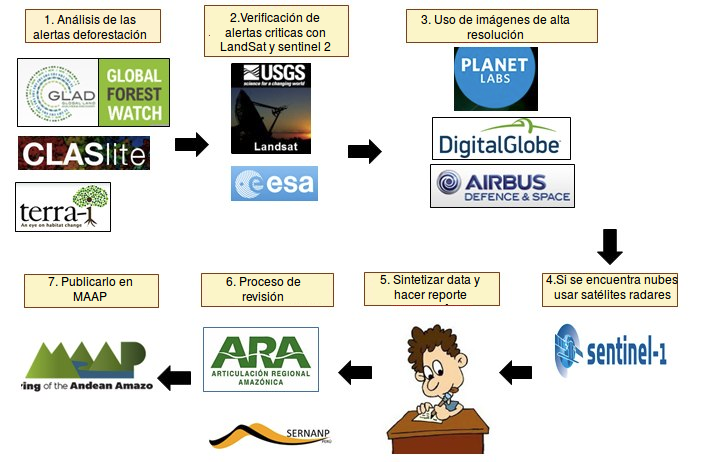
\includegraphics[width=0.8\textwidth]{images/MetologiaMAAPv2.png}
\caption{Metodología de \gls{MAAP} traducida de \cite{AmazonConservation} }
\label{maap}

\end{figure}

Algunos de los sistemas de detección de cambios usados para el análisis forestal en el Perú están basados en imágenes de mediana resolución adquiridas mediante convenio con instituciones extranjeras, al hacer un análisis más detallado de las zonas deforestadas se evidencia que las imágenes de mediana resolución(15 metros) no son suficientes \cite{hansen2013high}.

La detección de cambios en imágenes multitemporales es un problema clásico de la teledetección \cite{Zhu2017}, se han desarrollado varios trabajos que tratan de analizar los cambios con técnicas de procesamiento de imágenes tradicionales\cite{hansen2013high,AlenCastro2015,Anwar2012,Hirschmugl2014,Zhu2014}, sin embargo el uso del aprendizaje profundo aun tiene bastante campo de estudio.













\section{Formulación del Problema}
La detección de cambios realizada manualmente por humanos es una tarea que requiere de mucho esfuerzo y muchas veces esta tarea es susceptible a errores. Aunque existen plataformas de software en Perú que realizan un análisis de deforestación, estas aun presentan procesos manuales.

\section{Objetivo de la Investigación}
\subsection{Objetivo General}
Realizar un modelo computacional para la detección de cambios de la selva amazónica usando imágenes satélites multiespectrales mediante un enfoque de aprendizaje profundo.

\subsection{Objetivos Específicos}
\begin{itemize}[$\circ$]

% \item Estudiar las distintas causas de la deforestación.
  \item Elaborar una base de datos de imágenes satelitales.


 \item Construir un modelo de red neuronal profunda que permita la segmentación semántica de cada imagen.

 \item Elaborar un modelo que permita realizar un mapa de cambios basado en la segmentación semántica. 
    \item Análisis de los resultados.
\end{itemize}

\section{Hipótesis de la Investigación}
Un modelo computacional basado en las redes neuronales profundas será capaz de detectar cambios en imágenes satelitales multitemporales.

\section{Variables e Indicadores}
\subsection{Variable Independiente}
\begin{itemize}
    \item  Cambios planteados por la herramienta MAAP.
    \item  Imágenes Satelitales
    \item Zonas de adquisición.
\end{itemize}

\subsection{Variable Dependiente}
\begin{itemize}
    \item Presencia de cambios(Medio, medio-Alto, Alto): Esto representa que tan grande fue la deforestación en un área determinada.

    \item \textbf{IoU:} este es el método estándar de evaluación, calcula la relación entre la intersección y la unión de dos conjuntos, en segmentación esto es la relación entre nuestro \textbf{ground truth} y nuestra predicción \cite{GarciaGarcia2017}.
    \item \textbf{Accuracy:} Calcula la relación entre el total de pixeles correctamente clasificados y el total de pixeles \cite{GarciaGarcia2017}.
    
\end{itemize}{}

\section{Viabilidad de la Investigación}
\subsection{Viabilidad Técnica}
Como se menciona en \cite{long2015fully} es posible realizar una segmentación semántica mediante redes neuronales convolucionales, y  en el trabajo de \cite{Doshi2018} el uso de redes neuronales convolucionales en la detección de cambios es viable. 

\subsection{Viabilidad Operativa}
El modelo puede ser utilizado por las entidades del estado para la detección de cambios automatizada, sin embargo la propuesta no sera utilizable a gran escala sin una plataforma que gestione las propiedades de las imágenes, el acceso a datos y equipos. El proyecto de \textbf{Sistema de soporte a la toma de decisiones para el manejo forestal, utilizando imágenes satelitales y computación de alto desempeño - IDIBIO-118} propone una plataforma que albergará el proyecto.


\subsection{Viabilidad Económica}
La obtención de las imágenes será mediante la plataforma Planet, esta plataforma da acceso a una cierta cantidad de imágenes gratuitas con fines académicos. Además el proyecto de tesis cuenta con la financiación del proyecto: \textbf{Sistema de soporte a la toma de decisiones para el manejo forestal, utilizando imágenes satelitales y computación de alto desempeño - IDIBIO-118} que financiará los costos asociados




\section{Justificación e Importancia de la Investigación}
\subsection{Justificación}
Se puede entender a la deforestación como el proceso por el cual la superficie forestal es destruida, de esta manera la detección de cambios puede ser usada como un método de detección de deforestación.   

%El cambio de suelos da un indicio de como se da el proceso de deforestación, es por eso que la detección de cambios provee información de soporte para la prevención de la deforestación.

%Encontrar zonas deforestadas puede ser difícil si se trata de realizar mediante una exploración desde el suelo, es por eso que en la actualidad se usan distintas herramientas como imágenes satelitales, fotografías áreas, etc. 

Las imágenes satelitales son de gran ayuda para el análisis de suelos, estas imágenes pueden llegar a zonas donde el acceso es difícil \cite{AlenCastro2015}. El uso de imágenes satelitales es una solución más barata en comparación a la toma de fotografías aéreas, además las imágenes satelitales cuentan con más información que la obtenida mediante la vista humana \cite{unsalan2013multispectral}.


Hace algunos años la adquisición de imágenes satelitales era un problema, actualmente se cuenta con varios repositorios de imágenes libres como son: Earth Obsevation System\footnote{https://eos.com/}, Planet\footnote{https://www.planet.com/} o United States Geological Survey Digital Spectral Library\footnote{https://speclab.cr.usgs.gov/spectral-lib.html}; también existen algunas fuentes de datos libres como las del concurso ``Understanding the Amazon from Space'' de Kaggle\footnote{https://www.kaggle.com/c/planet-understanding-the-amazon-from-space}. 


El Perú adquirió un satélite de alta resolución llamado PeruSat que provee amplia información para los distintos estudios que se deseen realizar, para solicitar imágenes de PeruSat solo es necesario establecer un convenio con CONIDA (Comisión Nacional de Investigación y Desarrollo Aeroespacial).

Las técnicas de aprendizaje profundo han sido usadas en distintas tareas, recientemente se ha comenzado a usar estas técnicas en la teledetección \cite{zhang2016deep} debido a las ventajas que ofrece en problemas de alta dificultad, en cuyos casos no es posible una extracción de características apropiada.

 El aprendizaje profundo es un enfoque en el cual las características no son preprocesadas, el enfoque profundo puede ser útil para el problema de la detección de cambios, dado que se evita este preprocesamiento.
\subsection{Importancia}
La importancia de la investigación radica en que al automatizar el proceso de detección de cambios esta  puede aumentar la velocidad del proceso y lograr un mejor desempeño al momento de tomar las acciones necesarias por parte de las entidades gubernamentales correspondientes.
\section{Limitaciones de la Investigación}
La resolución espacial de las imágenes satelitales y/o la presencia de cultivos y/o pasto en las imágenes satelitales puede llegar a limitar el resultado del modelo. Además se tiene que considerar que la presencia de nubes y neblina limita la correcta visualización de las escenas y además se requiere de equipos de alta capacidad de procesamiento. 
\section{Tipo y Nivel de la Investigación}
\subsection{Tipo de Investigación}
Según \cite{hernandez2010metodologia} el enfoque de la investigación vendría a ser del tipo cuantitativo  debido a que la investigación tiene las siguientes características:
\begin{itemize}
    \item El problema ya esta delimitado.
    \item Se ha realizado la revisión del estado del arte una vez definido el problema.
    \item Se construyó un hipótesis en base a la revisión del estado del arte.
    \item Las imágenes son consideradas como matrices de números.
\end{itemize}{}

\subsection{Nivel de la Investigación}
El nivel de la investigación es exploratoria debido a que se parte de un campo estudiado como las redes neuronales convolucionales y se explora el conocimiento hacia una nueva area como son los modelos de sistema de detección de cambios en Perú.

\section{Método y Diseño de la Investigación}
\subsection{Método de la Investigación}
Como se menciona en ~\cite{long2015fully} el uso de las redes neuronales para la clasificación de imágenes es de bastante importancia desde que el trabajo de~\cite{krizhevsky2012imagenet} en 2012 ganó el concurso Imagenet\footnote{ImageNet es una base de datos de imágenes organizada según la jerarquía de WordNet (actualmente solo los sustantivos), en la que cada nodo de la jerarquía está representado por cientos y miles de imágenes. Actualmente se tiene un promedio de más de quinientas imágenes por nodo.} que consistía en etiquetar imágenes, a partir de eso distintos trabajos comenzaron a hacer el uso de las redes neuronales convolucionales para etiquetado de imágenes y para la detección de objetos.
El próximo paso fue la inferencia de cada pixel, los primeros intentos para la segmentación semántica~\cite{ning2005toward,   ciresan2012deep, farabet2013learning} realizaban una clasificación para cada uno de los pixeles tomando en cuenta una ventana, es decir se utilizaba una red neuronal para cada pixel. Usar una red neuronal para clasificar cada uno de los pixeles es bastante costoso,se menciona que la red propuesta en \cite{krizhevsky2012imagenet}  realiza la tarea de clasificación de una imagen de 224x224 en 1.2 ms mientras que la arquitectura propuesta en \cite{long2015fully} puede generar una grilla de 10x10 de una imagen de 500x500 en 22 ms logrando asi una velocidad 5 veces mayor al de clasificar cada pixel.

\subsection{Diseño de la investigación}
\label{sec:MetodologiaElvis}
La detección de cambios se hará utilizando técnicas de aprendizaje profundo.

La investigación se dividirá en 3 etapas. 
\begin{enumerate}
\item La primera etapa sera la construcción de una base de datos apropiada incluye:
\begin{itemize}
 \item Recolección de imágenes satelitales de distintas fuentes (Kaggle, Planet, PeruSat).
 \item Procesamiento de las imágenes para correcciones geométricas o atmosféricas.
 \item Segmentación manual de las imágenes con su respectivo etiquetado. 
\end{itemize}
\item En la segunda etapa se construirá un modelo de red convolucional para poder realizar un segmentado semántico a cada uno de los pixeles de las imágenes.

%http://lema.rae.es/dpd/srv/search?key=p%EDxel
\begin{figure}[H]
    \centering
    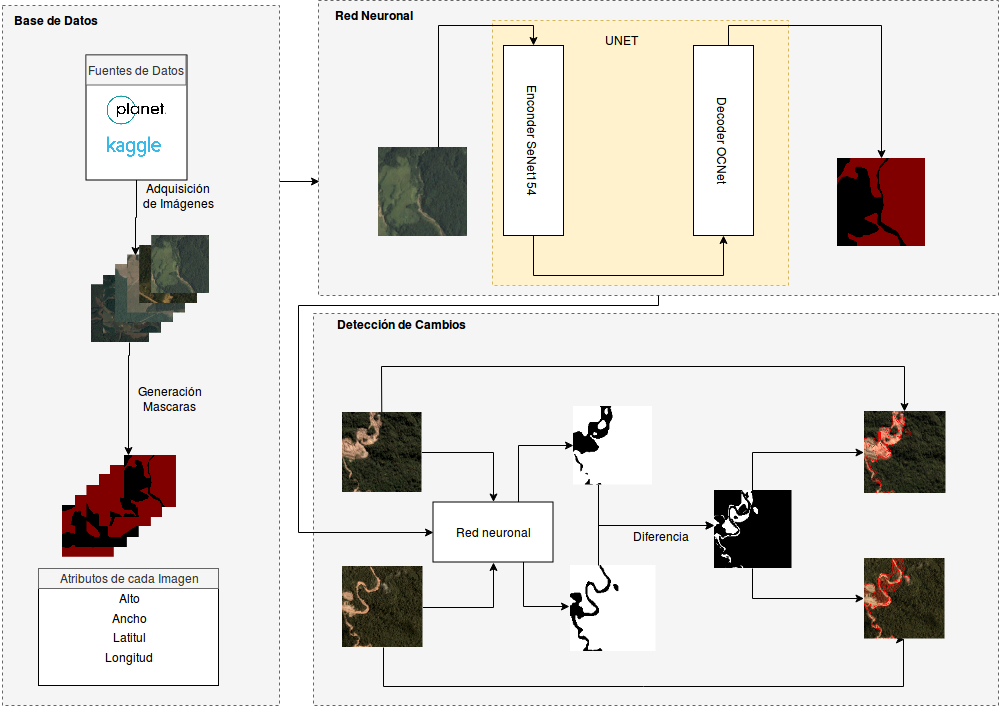
\includegraphics[width=0.8\textwidth]{images/ArquitecturaFinakl.png}
    \caption{Gráfico de la metodología}
    \label{fig:my_label}
\end{figure}
\item En la tercera etapa se seleccionara la mejor configuración de red construir un modelo computacional de detección de cambios basado en el artículo de \cite{doshi2018satellite} para obtener una imagen segmentada.
\end{enumerate}
\section{Técnicas e Instrumentos de Recolección de Información}

\subsection{Técnicas}
Para la obtención de las imágenes satelitales se plantea la búsqueda en la web de repositorios libres de imágenes, además de utilizar el sistema de descargas de imágenes oficiales de la página de Planet\footnote{www.planet.com}. 


\subsection{Instrumentos}
Se usarán frameworks de desarrollo que habilitarán la construcción de las redes neuronales profundas como pueden ser \textbf{Pytorch\footnote{https://pytorch.org/}, Tensorflow \footnote{https://www.tensorflow.org/} o Caffe\footnote{https://caffe.berkeleyvision.org/}}. Se verificará el estado del arte en concursos de segmentación semántica. Para la generación de máscaras se usará herramientas de etiquetado como es \textbf{Labelme\footnote{https://github.com/wkentaro/labelme}}.

\section{Organización del trabajo}
A continuación y a modo de guía de la lectura del documento, se describe la estructura de la tesis y los contenidos esenciales de cada capítulo.
En el capítulo \ref{chap:introduccion} (\textit{Introducción}) se especifica el planteamiento del problema, las variables dependiente e independiente, los objetivos, así como la metodología empleada, y la organización de la tesis. En el capítulo \ref{chap:marcoTeorico}(\textit{Marco Teórico:}) se desarrollarán los conceptos necesarios para poder entender la propuesta. En el capítulo \ref{chap:imagenes}(\textit{Base de datos de Imágenes Satelitales}) se detallará el proceso de construcción de la base de datos. capítulo \ref{chap:desarrollo}(\textit{Desarrollo}) se detalla el proceso de construcción del modelo propuesto. En el capítulo \ref{chap:pruebas} (\textit{Pruebas y resultados}) se describen las pruebas realizadas, los diferentes parámetros que se utilizaron, así como la validación de los resultados, la precisión. En el capítulo \ref{chap:conclusiones} (\textit{Conclusiones y trabajos futuros}): se dan las conclusiones finales de todo el trabajo realizado y se presentan líneas de trabajo que quedan abiertas a futuras investigaciones.



\chapter{Marco teórico}
\label{chap:marcoTeorico}
En esta parte se presentan los principales conceptos que serán utilizados en la tesis.
\section{Deforestación}


 Según~\cite{geist2002proximate} se formularon varias hipótesis para definir las causas de la deforestación cada una producidas en base de buenos argumentos, pero la evidencia empírica sobre las causas de la deforestación sigue basándose en gran medida en análisis de estadísticas nacionales. En algunos casos, estos análisis se basan en datos discutibles sobre las tasas de cambio de la cubierta forestal. 
 
 
Según el estudio~\cite{mena2010respuestas} la deforestación de la selva amazónica se debe a: 
 \begin{itemize}
  \item \textbf{Caminos y carreteras}: Las carreteras son herramientas indispensables para el desarrollo~\cite{dourojeanni2009amazonia}. La construcción de carreteras tiene dos objetivos que siempre están presentes: (i) unir dos localidades o regiones entre las cuales hay necesidad de transportar gente y productos y, (ii) tornar viable o económicamente viable el acceso a la tierra y al transporte de productos en ella generados mediante la agricultura y la explotación de bosques, minas, fauna y otros recursos. Estos objetivos son razonables en la medida que sean respetados los límites para el uso de la tierra y los recursos preestablecidos mediante el planeamiento y la legislación. El impacto socio ambiental de las carreteras deriva de la falta de ese planeamiento y/o de la falta de cumplimiento de la legislación. 
 \item \textbf{Extracción de madera: }En este tema, en teoría, hay que diferenciar dos situaciones: (i) la explotación forestal legal, sobre la base de concesiones forestales de acuerdo a ley, y (ii) la explotación ilegal. Si la explotación forestal legal fuera bien hecha, aplicando planes de manejo que garanticen la sostenibilidad del bosque, no se necesitaría incluir este tema en el contexto de este estudio. El problema es que, a pesar de las buenas intenciones del gobierno y de muy pocos empresarios, la explotación en concesiones forestales es irracional, insostenible y perjudicial en términos ambientales y sociales como la que es completamente informal. Apenas cambia la escala. 
 \item \textbf{Incendios: }Las áreas de fuego, definidas como el radio de diez kilómetros de un foco detectado por satélite, cubren aproximadamente un tercio de la Amazonía brasileña. Estas áreas están vinculadas, en dos tercios de los casos, a zonas deforestadas y urbanas, y el resto a áreas de manejo por parte de comunidades nativas y mestizas, a zonas de tala selectiva (el cincuenta por ciento de las áreas autorizadas por el gobierno están afectadas), y a la concentración de rutas no oficiales\cite{barreto2006human} .En muchos casos esos fuegos corresponden a la vieja práctica del ``chaqueo'': la tala y quema de los predios, preparándolos para el cultivo.En el caso de Bolivia, la práctica sigue muy extendida, y se generan miles de incendios cuyo humo cubre el norte del país y las regiones adyacentes de Brasil
\item \textbf{Agricultura: }La agricultura intensiva es deseable en la medida en que su expansión se haga a costa de las tierras semi-abandonadas en rotaciones extensas o de las que se usan para ganadería extensiva o sobre pastos degradados~\cite{dourojeanni2009amazonia}. En efecto, el uso de tecnología moderna, inclusive maquinaria y agroquímicos para mejorar el suelo (calcáreo y fertilizante) permite reusar tierras abandonadas por la agricultura, lo que es tradicional en la Amazonía. En cambio, sus ventajas son dudosas o nulas si la agricultura intensiva para biocombustibles o para exportación se hace destruyendo bosques naturales directa o indirectamente. Cualquier tipo de agricultura, pero especialmente la intensiva, trae aparejados problemas ambientales bien conocidos (Cuadro 18), en especial los derivados de la contaminación de suelos y agua por uso, frecuentemente abusivo, de agroquímicos diversos (fertilizantes, pesticidas, herbicidas) y, casi siempre, problemas serios de erosión hídrica por manejo deficiente de los suelos41. Pero, en términos generales, la agricultura intensiva no es peor que la agricultura tradicional en los trópicos húmedos, o sea, la de “roza y quema” o migratoria. En teoría puede, inclusive, ser ambientalmente menos agresiva ya que, en general, se desarrolla legalmente en un ámbito fijo año tras año, con productividad mucho mayor pues no aplica
\item \textbf{Energía: }
La exploración y explotación de hidrocarburos abarca áreas muy extensas pero con una intensidad relativamente baja y, en términos de deforestación es mucho menos impactante que otras explotaciones o infraestructuras. Sin embargo, sus impactos ambientales y sociales pueden ser muy serios, en especial los referentes a la contaminación de los cursos de agua~\cite{dourojeanni2009amazonia}. La contaminación se produce principalmente por la disposición inadecuada de las aguas de formación que cargan una serie de sustancias altamente tóxicas, como plomo, cadmio, arsénico y mercurio, entre otros o conocidos carcinógenos como tolueno y benceno, y asimismo por derrames de crudo en los pozos y dentro de cada lote y, especialmente durante su transporte por gasoductos y oleoductos hasta las localidades de  procesamiento o consumo
  
 \end{itemize}


Según un estudio en la Selva de Brasil del Instituto Nacional de Pesquisas de la Amazonia las causas de la deforestación son~\cite{fearnside2005deforestation}:
\begin{itemize}
\item Perdida de la productividad.
\item Cambios en el régimen hidrológico.
\item Perdida de la biodiversidad.
\item Emisiones netas de gases de efecto invernadero-

\end{itemize}
\section{Espectro Electromagnético}
La radiación electromagnética es un tipo de campo electromagnético variable, es decir, una combinación de campos eléctricos y magnéticos oscilantes, que se propagan a través del espacio transportando energía de un lugar a otro~\cite{Feynman}. Las ondas electromagnéticas que componen la radiación electromagnética pueden ser representadas como campos eléctricos y magnéticos autopropagados en forma de onda transversa. Se denomina espectro electromagnético a la distribución energética del conjunto de las ondas electromagnéticas. 
 \begin{figure}[H]
\centering
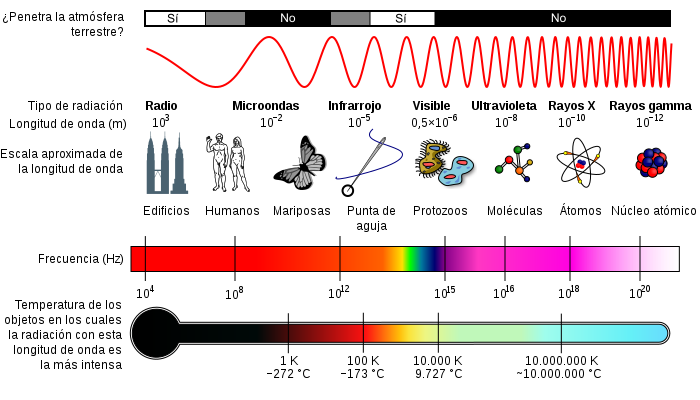
\includegraphics[width=0.75\textwidth]{images/espectro.png}
\caption{Espectro Electromagnético adaptada por~\cite{wikies} de~\cite{NASAEspectro} en la que se muestra la longitud de onda de cada agrupación}

\end{figure}
\section{Resolución} 
La resolución de una imagen indica la cantidad de detalles que puede observarse en esta. Tener mayor resolución se traduce en obtener una imagen con más detalle o calidad visual. Según~\cite{Wulder1998} la resolución es la medida de variación de un sensor para conseguir un valor.
\begin{itemize}
 \item \textbf{Resolución Espacial}\newline
Es la cantidad de información que representa un pixel~\cite{Wulder1998}, siendo el caso que un objeto puede estar representado por un solo pixel de 100 metros cuadrados o por 100 pixeles de 1 metro cuadrado. 
\begin{figure}[H]
    \centering
    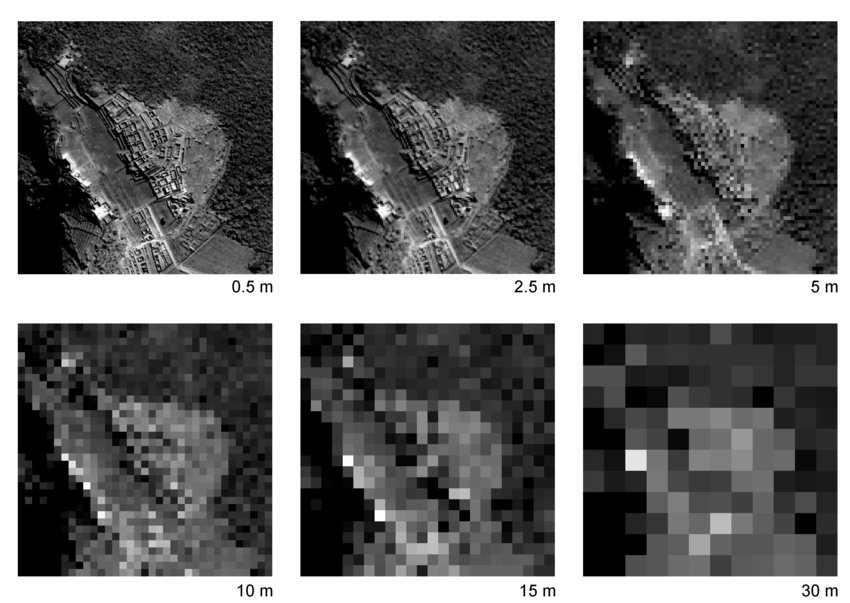
\includegraphics[width = 0.8\textwidth]{images/02theory/espacial.png}
    \caption{Distintas resoluciones espaciales para la misma zona}
    \label{fig:resolucionEspacial}
\end{figure}

Como se aprecia en la \figurename~\ref{fig:resolucionEspacial} cuando se tiene una mayor resolución espacial los objetos tienen un mayor grado de detalle.


\item \textbf{Resolución Espectral}\newline
 Hace referencia a la cantidad del espectro electromagnético se esta midiendo y en cuantos canales se separa, es decir que si la imagen fue tomada en un amplio espectro y el tamaño de los canales es corto tendrá una mejor resolución espectral~\cite{wulder2012remote}.
 \begin{figure}[H]
     \centering
     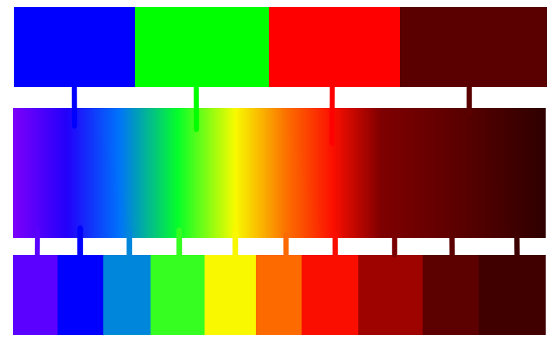
\includegraphics[width=0.6\textwidth]{images/02theory/resolucionespectralCortada.png}
     \caption[Resolución espectral]{Se muestra que en determinado rango del espectro electromagnético se puede usar divisiones más pequeñas para obtener más canales espectrales o mejor resolución espectral}
     \label{fig:resolucionEspectral}
 \end{figure}
 
 
\item \textbf{Resolución Temporal}\newline
 Se toma en cuenta que la resolución temporal es la frecuencia por la que un satélite puede tomar información de una zona~\cite{Wulder1998}.
\begin{figure}[H]
    \centering
    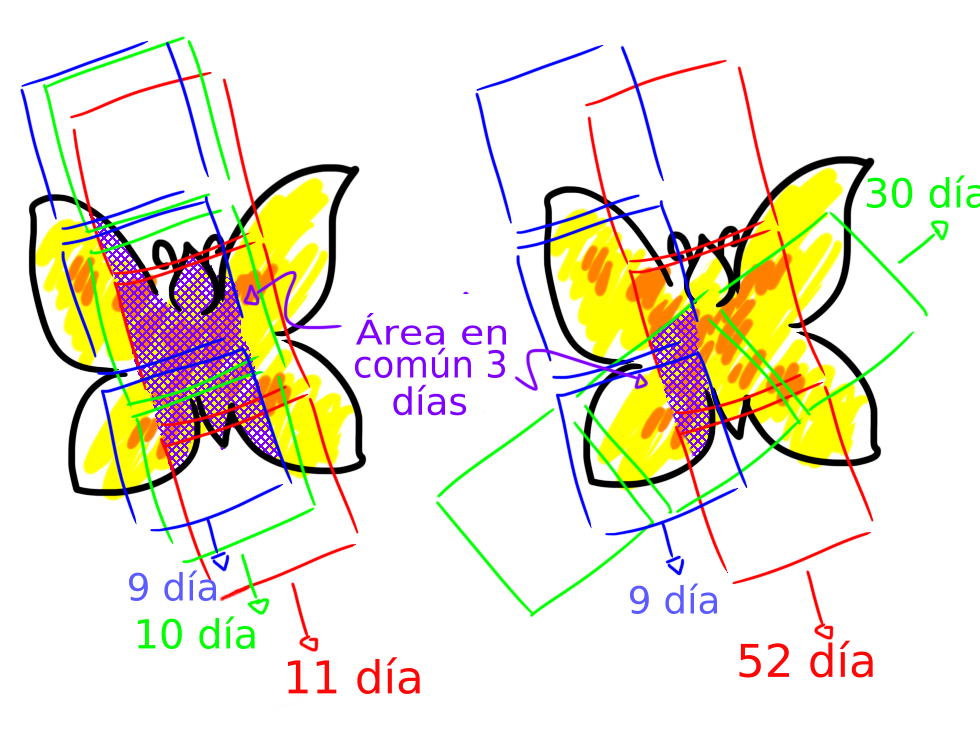
\includegraphics[width=0.5\textwidth]{images/02theory/resolucionTemporalEspa.png}
    \caption[Resolución Radiométrica]{Resolución Temporal: Como se muestra en la figura la mejora de la resolución temporal facilitara la obtención de información multitemporal de una zona}
    \label{fig:my_label}
\end{figure} 
 
\item \textbf{Resolución Radiométrica}\newline
Se refiere a la cantidad de bits usados para representar la información, esto determinará que tan selectivo es el sensor~\cite{wulder2012remote}. 
\begin{figure}[H]
    \centering
    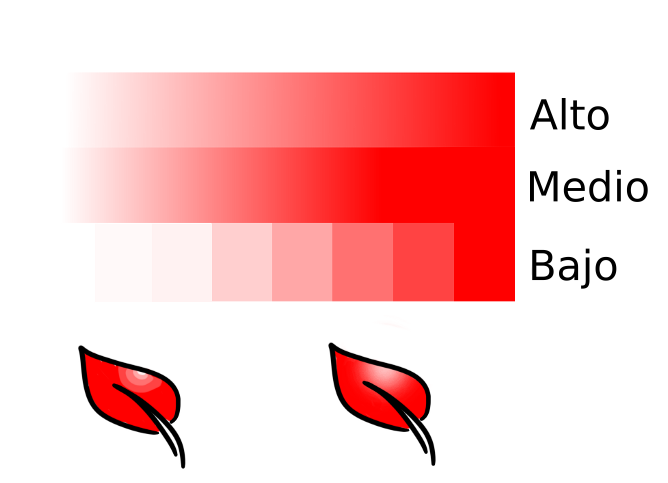
\includegraphics[width=0.6\textwidth]{images/02theory/resolucionRadiometrica.png}
    \caption[Resolución Radiométrica]{Resolución Radiométrica: Como se muestra en la hoja izquierda mientras menor sea la resolución radiométrica menos tonalidades tendremos de un valor}
    \label{fig:my_label}
\end{figure}
\end{itemize}

\section{Teledetección }
La Teledetección es una técnica por medio de la cual se obtiene información útil de un objeto, área o fenómeno, a través del análisis e interpretación de datos adquiridos por un equipo que no está en contacto físico con el objeto, área o fenómeno bajo investigación~\cite{jensen1987introductory}. 


La Teledetección espacial es una técnica que permite adquirir información de la superficie terrestre o marina y la atmósfera desde sensores instalados en plataformas espaciales, por ser una técnica que no esta en contacto directo con el objeto requiere que entre el sensor y el objeto haya un flujo de información.
\subsection{Usos}
Según el Servicio Geológico de los Estados Unidos algunos usos de la teledetección son~\cite{USGS}:
\begin{itemize}
 \item Las cámaras en satélites y aviones toman imágenes de grandes áreas en la superficie de la Tierra, lo que nos permite ver mucho más de lo que podemos desde una vista desde el suelo.
 \item Los sistemas de sonar en los barcos se pueden usar para crear imágenes del fondo del océano sin necesidad de viajar al fondo del océano.
  \item Se pueden usar cámaras en satélites para hacer imágenes de los cambios de temperatura en los océanos.
\end{itemize}
Algunos usos específicos de las imágenes satelitales de la tierra son: 
\begin{itemize}

 \item Los incendios forestales grandes pueden ser mapeados desde el espacio, permitiendo a los guardabosques ver un área mucho mayor que desde el suelo.
 \item Rastrear nubes para ayudar a predecir el clima u observar volcanes en erupción, y ayudar a observar tormentas de polvo.
 \item Rastrear el crecimiento de una ciudad y los cambios en tierras de cultivo o bosques durante varios años o incluso décadas.
.
\end{itemize}
\subsection{Satélites de observación}
Los satélites de observación son satélites artificiales, su principal función de estos es la obtención de información mediante sensores, que pueden ser clasificados de 2 formas~\cite{campbell2011introduction}: 
\begin{itemize}
 \item \textbf{Activos} Generan su propia fuente de medición, ejemplo: 
 \begin{itemize}
  \item \textbf{SAR}\newline El SAR (Synthetic Aperture Radar en español radar de apertura sintética) es un radar activo que emite la energía en el intervalo de frecuencias de microondas en un período pequeño de tiempo y recibe los ecos provenientes de reflexiones de la señal en los objetos dando lugar a una apertura sintética~\cite{brown1967synthetic}. 
  \item \textbf{Lidar}\newline Un lídar (un acrónimo del inglés Light Detection and Ranging o Laser Imaging Detection and Ranging) es un dispositivo que permite determinar la distancia desde un emisor láser a un objeto o superficie. La distancia al objeto se determina midiendo el tiempo de retraso entre la emisión del pulso y su detección a través de la señal reflejada~\cite{Lim2003}.
  
 \end{itemize}
 \item \textbf{Pasivos} Estos obtienen información midiendo energía externa, ejemplo: \begin{itemize}
  \item \textbf{Satélites Ópticos}\newline En este caso la energía creado por el sol reflejada de la tierra es medida usando sensores, luego la información recobrada es usada para la construcción de una nueva imagen~\cite{elachi2006introduction}. La información obtenida usualmente esta fuera del rango del espectro electromagnético visto por el hombre.
 \end{itemize}
 
\end{itemize}
 
\subsection{Imágenes satelitales}
Una imagen satelital o imagen de satélite es la representación de la información capturada por un satélite~\cite{leon2002introduccion}.

\extrarowheight = -0.5ex
\renewcommand{\arraystretch}{2.25}
 \begin{table}[H]
\centering

\caption{Tabla de satélites adaptado de~\cite{unsalan2013multispectral}}
\resizebox{16cm}{!}{% <------ Don't forget this %
\begin{tabular}{|M{0.14\textwidth}|M{0.16\textwidth}|
   M{0.15\textwidth}|M{0.15\textwidth}|
   M{0.14\textwidth}|M{0.25\textwidth}|}
   \hline
 \cellcolor[HTML]{dcdcdc}\color[HTML]{000000} \textbf{Sensor} &
 \cellcolor[HTML]{dcdcdc}\color[HTML]{000000} \textbf{Resolución Espacial} Pancromática ($\SI{}{\metre}$) &
 
\cellcolor[HTML]{dcdcdc}\color[HTML]{000000} \textbf{Resolución Espacial Multiespectral ($\SI{}{\metre}$)} &

\cellcolor[HTML]{dcdcdc}\color[HTML]{000000} \textbf{Resolución Espectral ($ \SI{}{\micro\metre}$)} & 
\cellcolor[HTML]{dcdcdc}\color[HTML]{000000} \textbf{Resolución Temporal (días) } & \cellcolor[HTML]{dcdcdc}\color[HTML]{000000} \textbf{Bandas }  \\
 \hline
 

Landsat & 15 &  30  & 0.45 a 2.35               &  16          & BGR, NIR, SWIR1, SWIR2, TIR, PAN           \\  
SPOT        & 2.5 &10         & 0.50 a 1.75        & 5   & BGR, NIR, PAN        \\  

IRS       & 5 &23.5        & 0.50 a 1.70        & 5 & BGR, NIR, PAN         \\  
 
IKONOS        & 1 & 4        & 0.45 a 0.85        &  3 & BGR, NIR, PAN           \\  
QuickBird       & 0.61 &2.44         & 0.45 a 0.90        & 3   & BGR, NIR, PAN          \\  

FormoSat        & 2  &8         & 0.45 a 0.90        & 1 &BGR, NIR, PAN          \\  

CartoSat        & 2.5& N/A        & N/A        & 5  & PAN      \\  

WorldView       & 0.46 & 1.8         & 0.40 a 1.04        & 1.1   & BGR, NIR, SWIR1, SWIR2, TIR, PAN         \\  
ALOS       & 2.5 & 10         & 0.42 a 0.89        & 2  & BGR, NIR, PAN         \\  

GeoEye        & 0.41  &1.65        & 0.45 a 0.90        & 3   &BGR, NIR, PAN           \\  
Airborne        & 1 a 25 & 1 a 25         & 0.42 a 14.00        & N/A    & 1 a 224       \\  
Sentinel        & 10 & 20 o 60         & 0.443 a 2.190        & 10   & BGR, NIR, SWIR1, SWIR2, TIR, PAN        \\  
PeruSat       & 0.7 & 2.8 & 0.45 a 0.89        & 0.5  & BGR, NIR, PAN     
\\\hline
\end{tabular}% <------ Don't forget this %
}

\label{tab}%
\end{table}%

\section{Inteligencia Artificial}
En el \tablename  ~\ref{cuadroIA} adaptado de~\cite{russell2004inteligencia} se muestran algunas definiciones de inteligencia artificial. Las que aparecen en la parte superior se refieren a procesos mentales y al razonamiento, mientras que las de la parte inferior aluden a la conducta. Las definiciones de la izquierda miden el éxito en términos de la fidelidad en la forma de actuar de los humanos, mientras que las de la derecha toman como referencia un concepto ideal de inteligencia, que llamaremos racionalidad. Un sistema es racional si hace lo correcto, en función de su conocimiento.


 \begin{table}[H]
\centering

\caption{Cuadro de definiciones de Inteligencia Artificial adaptado de~\cite{russell2004inteligencia}}
\label{cuadroIA}
\begin{tabular}{|M{0.45\textwidth}|M{0.45\textwidth}|}
   \hline
 \cellcolor[HTML]{dcdcdc}\color[HTML]{000000} \textbf{Sistemas que piensan como humanos} &
 \cellcolor[HTML]{dcdcdc}\color[HTML]{000000} \textbf{Sistemas que piensan racionalmente}
 
 \\ \hline
 \begin{itemize}
  \item El nuevo y excitante esfuerzo de hacer que los computadores piensen... máquinas con mentes, en el más amplio sentido literal~\cite{Haugeland1985}.
\item La automatización de] actividades que vinculamos con procesos de pensamiento humano, actividades como la toma de decisiones, resolución de problemas, aprendizaje...~\cite{bellman1978introduction}
 
 \end{itemize}
 

&
\begin{itemize}
 \item El estudio de las facultades mentales mediante el uso de modelos computacionales~\cite{charniak1985introduction}.
 \item El estudio de los cálculos que hacen posible percibir, razonar y actuar~\cite{winston1992learning}.
 
\end{itemize}
 \\ \hline
 \cellcolor[HTML]{dcdcdc}\color[HTML]{000000} \textbf{Sistemas que actúan como humanos
} 
&
 \cellcolor[HTML]{dcdcdc}\color[HTML]{000000} \textbf{Sistemas que actúan racionalmente}
 \\ \hline
 \begin{itemize}
  \item El arte de desarrollar máquinas con capacidad para realizar funciones que cuando son realizadas por personas requieren de inteligencia~\cite{kurzweil1990age}.
 \item El estudio de cómo lograr que los computadores realicen tareas que, por el momento, los humanos hacen mejor~\cite{rich1991artificial}.
 
 \end{itemize}
&
\begin{itemize}
 \item La Inteligencia Computacional es el estudio del diseño de agentes inteligentes.~\cite{poole1998computational}
 \item IA... está relacionada con conductas inteligentes en artefactos~\cite{nilsson1998artificial}.
\end{itemize}

 \\ 
\hline
\end{tabular}%

\label{tab:addlabel}%
\end{table}%
\subsection{Visión computacional}
La principal función de la visión es reconocer y localizar objetos en el ambiente mediante el procesamiento de las imágenes. La visión computacional es el estudio de estos procesos, para entenderlos y construir maquinas con capacidades similares~\cite{sucar2011vision}.
Algunas definiciones de visión son:
\begin{itemize}
  \item Visión es saber que hay y donde mediante la vista (Aristóteles).
  \item Visión es recuperar de la información de los sentidos (vista) propiedades validas del mundo exterior, Gibson~\cite{gibson2014ecological}.
  \item  Visión es un proceso que produce a partir de las imágenes del mundo exterior una descripción que es útil para el observador y que no tiene información irrelevante, Marr~\cite{marr1982vision}.
\end{itemize}
\subsection{Aprendizaje profundo}
Las RNA (redes neuronales artificiales) son modelos predictivos basados en la estructura biológica del cerebro humano. Una RNA se construye mediante la vinculación de entrada nodos con conexiones ponderadas a los nodos de salida a través de uno o más
capas de nodos ocultos~\cite{rumelhart1986learning}.


El aprendizaje profundo es un enfoque caracterizado por tener múltiples niveles que sirven para abstraer información de un conjunto de datos~\cite{lecun2015deep}. Una de las estructuras más utilizadas son las redes neuronales convolucionales.


En una red neuronal normal las entradas están desplegadas de manera lineal, es decir las redes son operadas linealmente hacia la siguiente capa. En el caso de una red neuronal convolucional las capas tienen más de una dimensión a esto se le conoce como capas convolucionales, esto provee información espacial que puede ser utilizada por la red neuronal para una mejor extracción de características. La forma en la cual se pasa información de una capa otra es mediante convoluciones que es la transformación de un valor a otro

\section{Redes Neuronales}
\subsection{Redes Neuronales Convencionales}
\label{section:marcoTeorico:redesneuronales}
Para~\cite{Haykin1994} una red neuronal o unidad de procesamiento es una máquina diseñada para modelar la forma en la que el cerebro realiza una actividad, la define además como un procesador distribuido masivamente paralelo formado por unidades de procesamiento simples (neuronas) que son propensos a almacenar conocimiento y ponerlo a disposición para su uso. Cada neurona recibe una serie de entradas a través de interconexiones y emite una salida. Se identifican 3 elementos básicos del modelo como sigue:
\begin{itemize}
\item Conjunto de sinapsis o enlaces de conexión que reemplazan a las conexiones sinápticas del cerebro humano, caracterizadas por tener un peso equivalente a la efectividad de la sinapsis, en específico con respecto al peso de una neurona en la~\figurename~\ref{figure:RedNeuronal}, en $w_{kj}$ el primer subíndice representa a la neurona propia, el segundo subíndice se refiere a la señal de entrada, formando así el peso neuronal.
\item Una función de propagación o de red, consiste en la sumatoria de cada entrada multiplicada por el peso de su interconexión (valor neto). Si el peso es positivo, la conexión se denomina excitatoria; si es negativo, se denomina inhibitoria, las operaciones describen una combinación lineal.
\item Una función activación, que se aplica al valor devuelto por la función de propagación. Se utiliza para acotar la salida de la neurona y viene dada por la interpretación que se da a las salidas. Algunas de las más utilizadas son la función sigmoidea (para obtener valores en el intervalo [0, 1] y la tangente hiperbólica (para obtener valores en el intervalo [-1, 1]).
\end{itemize}

\begin{figure}[H]
  \centering
    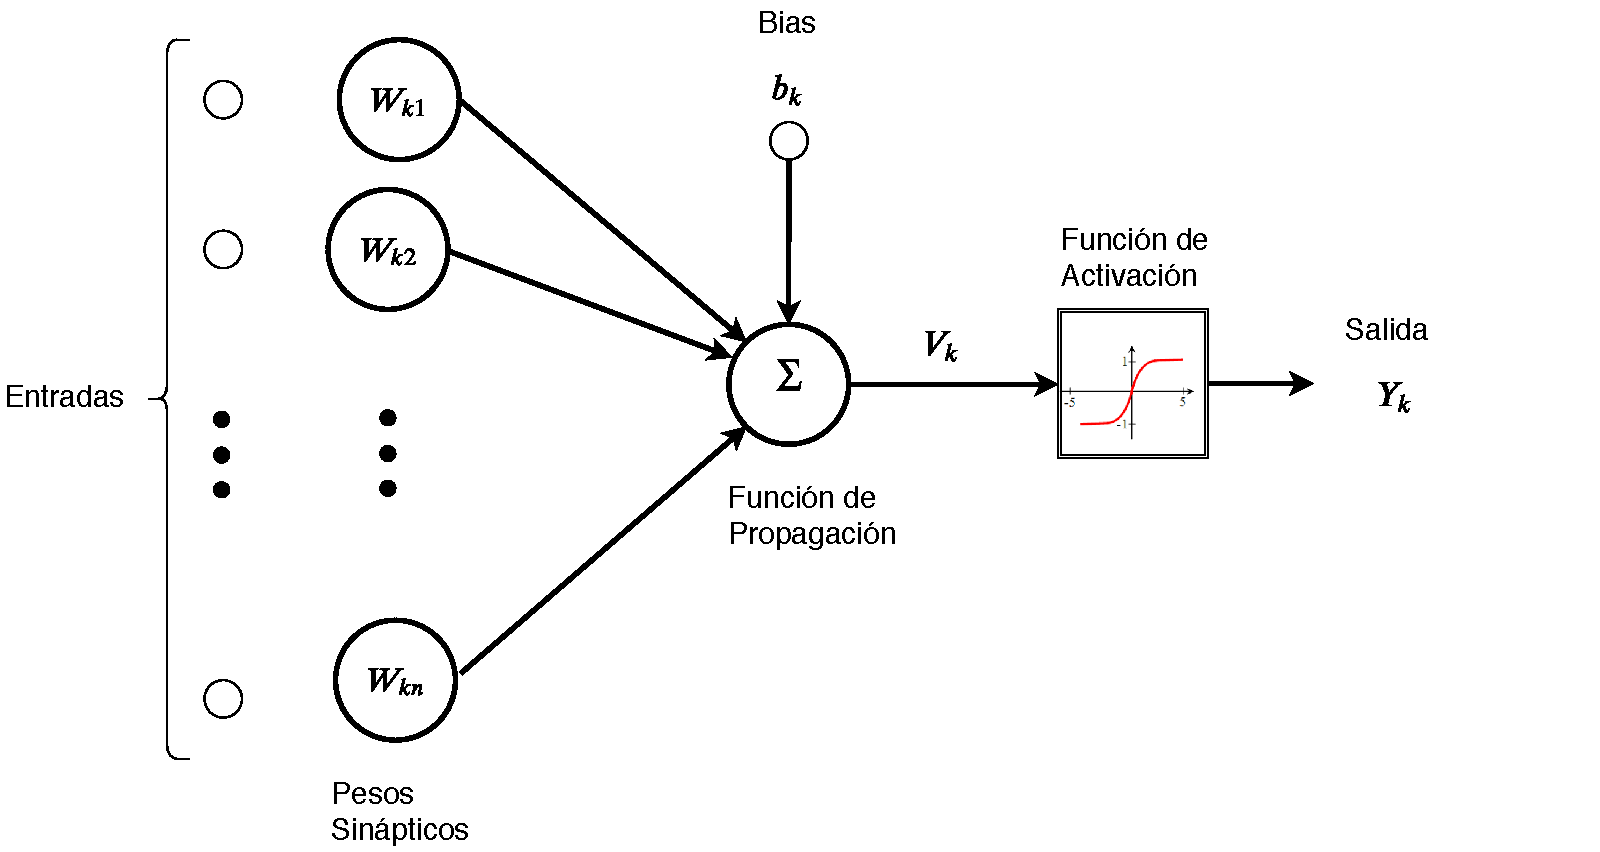
\includegraphics[width=0.9\textwidth]{images/redNeuronal.pdf}
  \caption[Arquitectura general Red Neuronal]{Modelo arquitectónico de una Red Neuronal adaptado de~\cite{Haykin1994}.}
  \label{figure:RedNeuronal}
\end{figure}

El modelo de red neuronal en la \figurename~\ref{figure:RedNeuronal} incluye un bias $b_{k}$, se puede describir la neurona $k$ con las siguientes ecuaciones:
\begin{equation}
  u_{k} = \sum_{j=1}^{n}x_{i} = w_{kj} \cdot x_{j}   
\end{equation}

\begin{equation}
  y_{k} =\varphi (u_{k}+b_{k})  
\end{equation}
\begin{equation}
  v_{k} = u_{k}+b_{k}  
\end{equation}

\subsection{Redes Neuronales Convolucionales}
 Una Red Neuronal Convolucional o \gls{CNN} por sus siglas en ingles (Convolutional Neural Network) es una red neuronal especial debido que procesa la data de manera topológica. Las \gls{CNN} han tenido tremendo éxito en aplicaciones prácticas, el nombre red convolucional  indica que la red emplea una operación matemática llamada convolución. La red neuronal convolucional es una red neuronal común que usa convoluciones en lugar de multiplicaciones matriciales en al menos alguna de sus capas.
\subsection{Función de perdida}
En el contexto de un algoritmo de optimización, la función utilizada para evaluar una solución candidata (es decir, un conjunto de ponderaciones) se conoce como la función objetivo.

Podemos buscar maximizar o minimizar la función objetivo, lo que significa que estamos buscando una solución candidata que tenga la puntuación más alta o más baja, respectivamente.

Normalmente, con las redes neuronales, buscamos minimizar el error. Como tal, la función objetivo a menudo se denomina función de costo o función de pérdida y el valor calculado por la función de pérdida se denomina simplemente "pérdida".
\subsection{Operaciones en redes Neuronales Convolucionales}
\subsubsection{Convolución }
\label{subsec:convolucion}

En el trabajo de \cite{Dumoulin2016} se mecían que la principal operación en las redes neuronales clásicas es la transformación afín: un vector se recibe como entrada y se multiplica con una matriz para producir una salida (a la que generalmente se agrega un vector de polarización antes de pasar el resultado a través de una no linealidad). Esto es aplicable a cualquier tipo de entrada, ya sea una imagen, un clip de sonido o una colección desordenada de características: sea cual sea su dimensionalidad, su representación siempre puede ser aplanada en un vector antes de la transformación. No obstante imágenes, clips de sonido y muchos otros tipos similares tienen una estructura intrínseca. Más formalmente, comparten estas importantes propiedades:
\begin{itemize}
    \item  Se almacenan como matrices multidimensionales.
\item Cuentan con uno o más ejes para los que es importante el ordenamiento (por ejemplo, ejes de ancho y alto para una imagen, eje de tiempo para un clip de sonido).
\item Un eje, llamado el eje del canal, se usa para acceder a diferentes vistas de los datos (por ejemplo, los canales rojo, verde y azul de una imagen en color, o los canales izquierdo y derecho de una pista de audio estéreo).
\end{itemize}

Estas propiedades no se explotan cuando se aplica una transformación afín, de hecho, todos los ejes se tratan de la misma manera y la información topológica no se tiene en cuenta. Sin embargo, aprovechar la estructura implícita de los datos puede resultar muy útil para resolver algunas tareas, como la visión artificial y el reconocimiento de voz, y en estos casos sería mejor preservarlo. Aquí es donde entran en juego las convoluciones discretas.Una convolución discreta es una transformación lineal que preserva esta noción de orden. Es esparcido (solo unas pocas unidades de entrada contribuyen a una unidad de salida determinada) y reutiliza los parámetros (los mismos pesos se aplican a múltiples ubicaciones en la entrada)
La \figurename~\ref{fig:convolucionArimetica} provee un ejemplo de lo que una convolución discreta. La grilla azul claro es llamada \gls{Feature Map} de entrada, pero es bastante común tener varios mapas de características amontonados uno sobre otro. Un \gls{kernel}(cuadrado plomo) pasa atreves del \gls{Feature Map} de entrada. En cada posición, se obtiene el producto entre cada uno de los elementos del \gls{kernel} y la entrada que se sobrelapan, el resultado final es obtenido sumando los resultados de los productos. Este proceso puede ser repetido con distintos \gls{kernel}s para formar diferentes \gls{Feature Map}s de salida. En caso de que se presenten varios \gls{Feature Map}s de entrada el \gls{kernel} tendrá que ser tridimensional (o equivalente a un \gls{kernel} por cada mapa de características de entrada).


%1 A kernel (shaded area) of value 
%slides across the input feature map. At each location, the product between
%each element of the kernel and the input element it overlaps is computed and
%the results are summed up to obtain the output in the current location. The
%procedure can be repeated using different kernels to form as many output feature
%maps as desired (Figure 1.3). The final outputs of this procedure are called
%output feature maps. 2 If there are multiple input feature maps, the kernel will
%have to be 3-dimensional – or, equivalently each one of the feature maps will
%be convolved with a distinct kernel – and the resulting feature maps will be
%summed up elementwise to produce the output feature map.
%The convolution depicted in Figure 1.1 is an instance of a 2-D convolution,
%but it can be generalized to N-D convolutions. For instance, in a 3-D convolu-
%tion, the kernel would be a cuboid and would slide across the height, width and
%depth of the input feature map.
%The collection of kernels defining a discrete convolution has a shape corre-
%sponding to some permutation of (n, m, k 1 , . . . , k N ), where
%n ≡ number of output feature maps,
%m ≡ number of input feature maps,
%k j ≡ kernel size along axis j.
%The following properties affect the output size o j of a convolutional \gls{Layer}
%along axis j:
%• i j : input size along axis j,
%• k j : kernel size along axis j,
%• s j : stride (distance between two consecutive positions of the kernel) along
%axis j,
%• p j : zero padding (number of zeros concatenated at the beginning and at
%the end of an axis) along axis j.
%For instance, Figure 1.2 shows a 3 × 3 kernel applied to a 5 × 5 input padded
%with a 1 × 1 border of zeros using 2 × 2 strides.
%Note that strides constitute a form of subsampling. As an alternative to
%being interpreted as a measure of how much the kernel is translated, strides can
%also be viewed as how much of the output is retained. For instance, moving
%the kernel by hops of two is equivalent to moving the kernel by hops of one but
%retaining only odd output elements (Figure 1.4).

\begin{figure}[H]
    \centering
    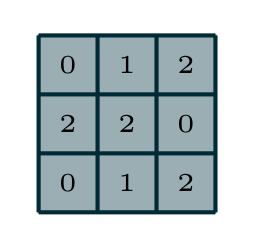
\includegraphics[width=0.2\textwidth]{images/convolucion/featuremap.png}
    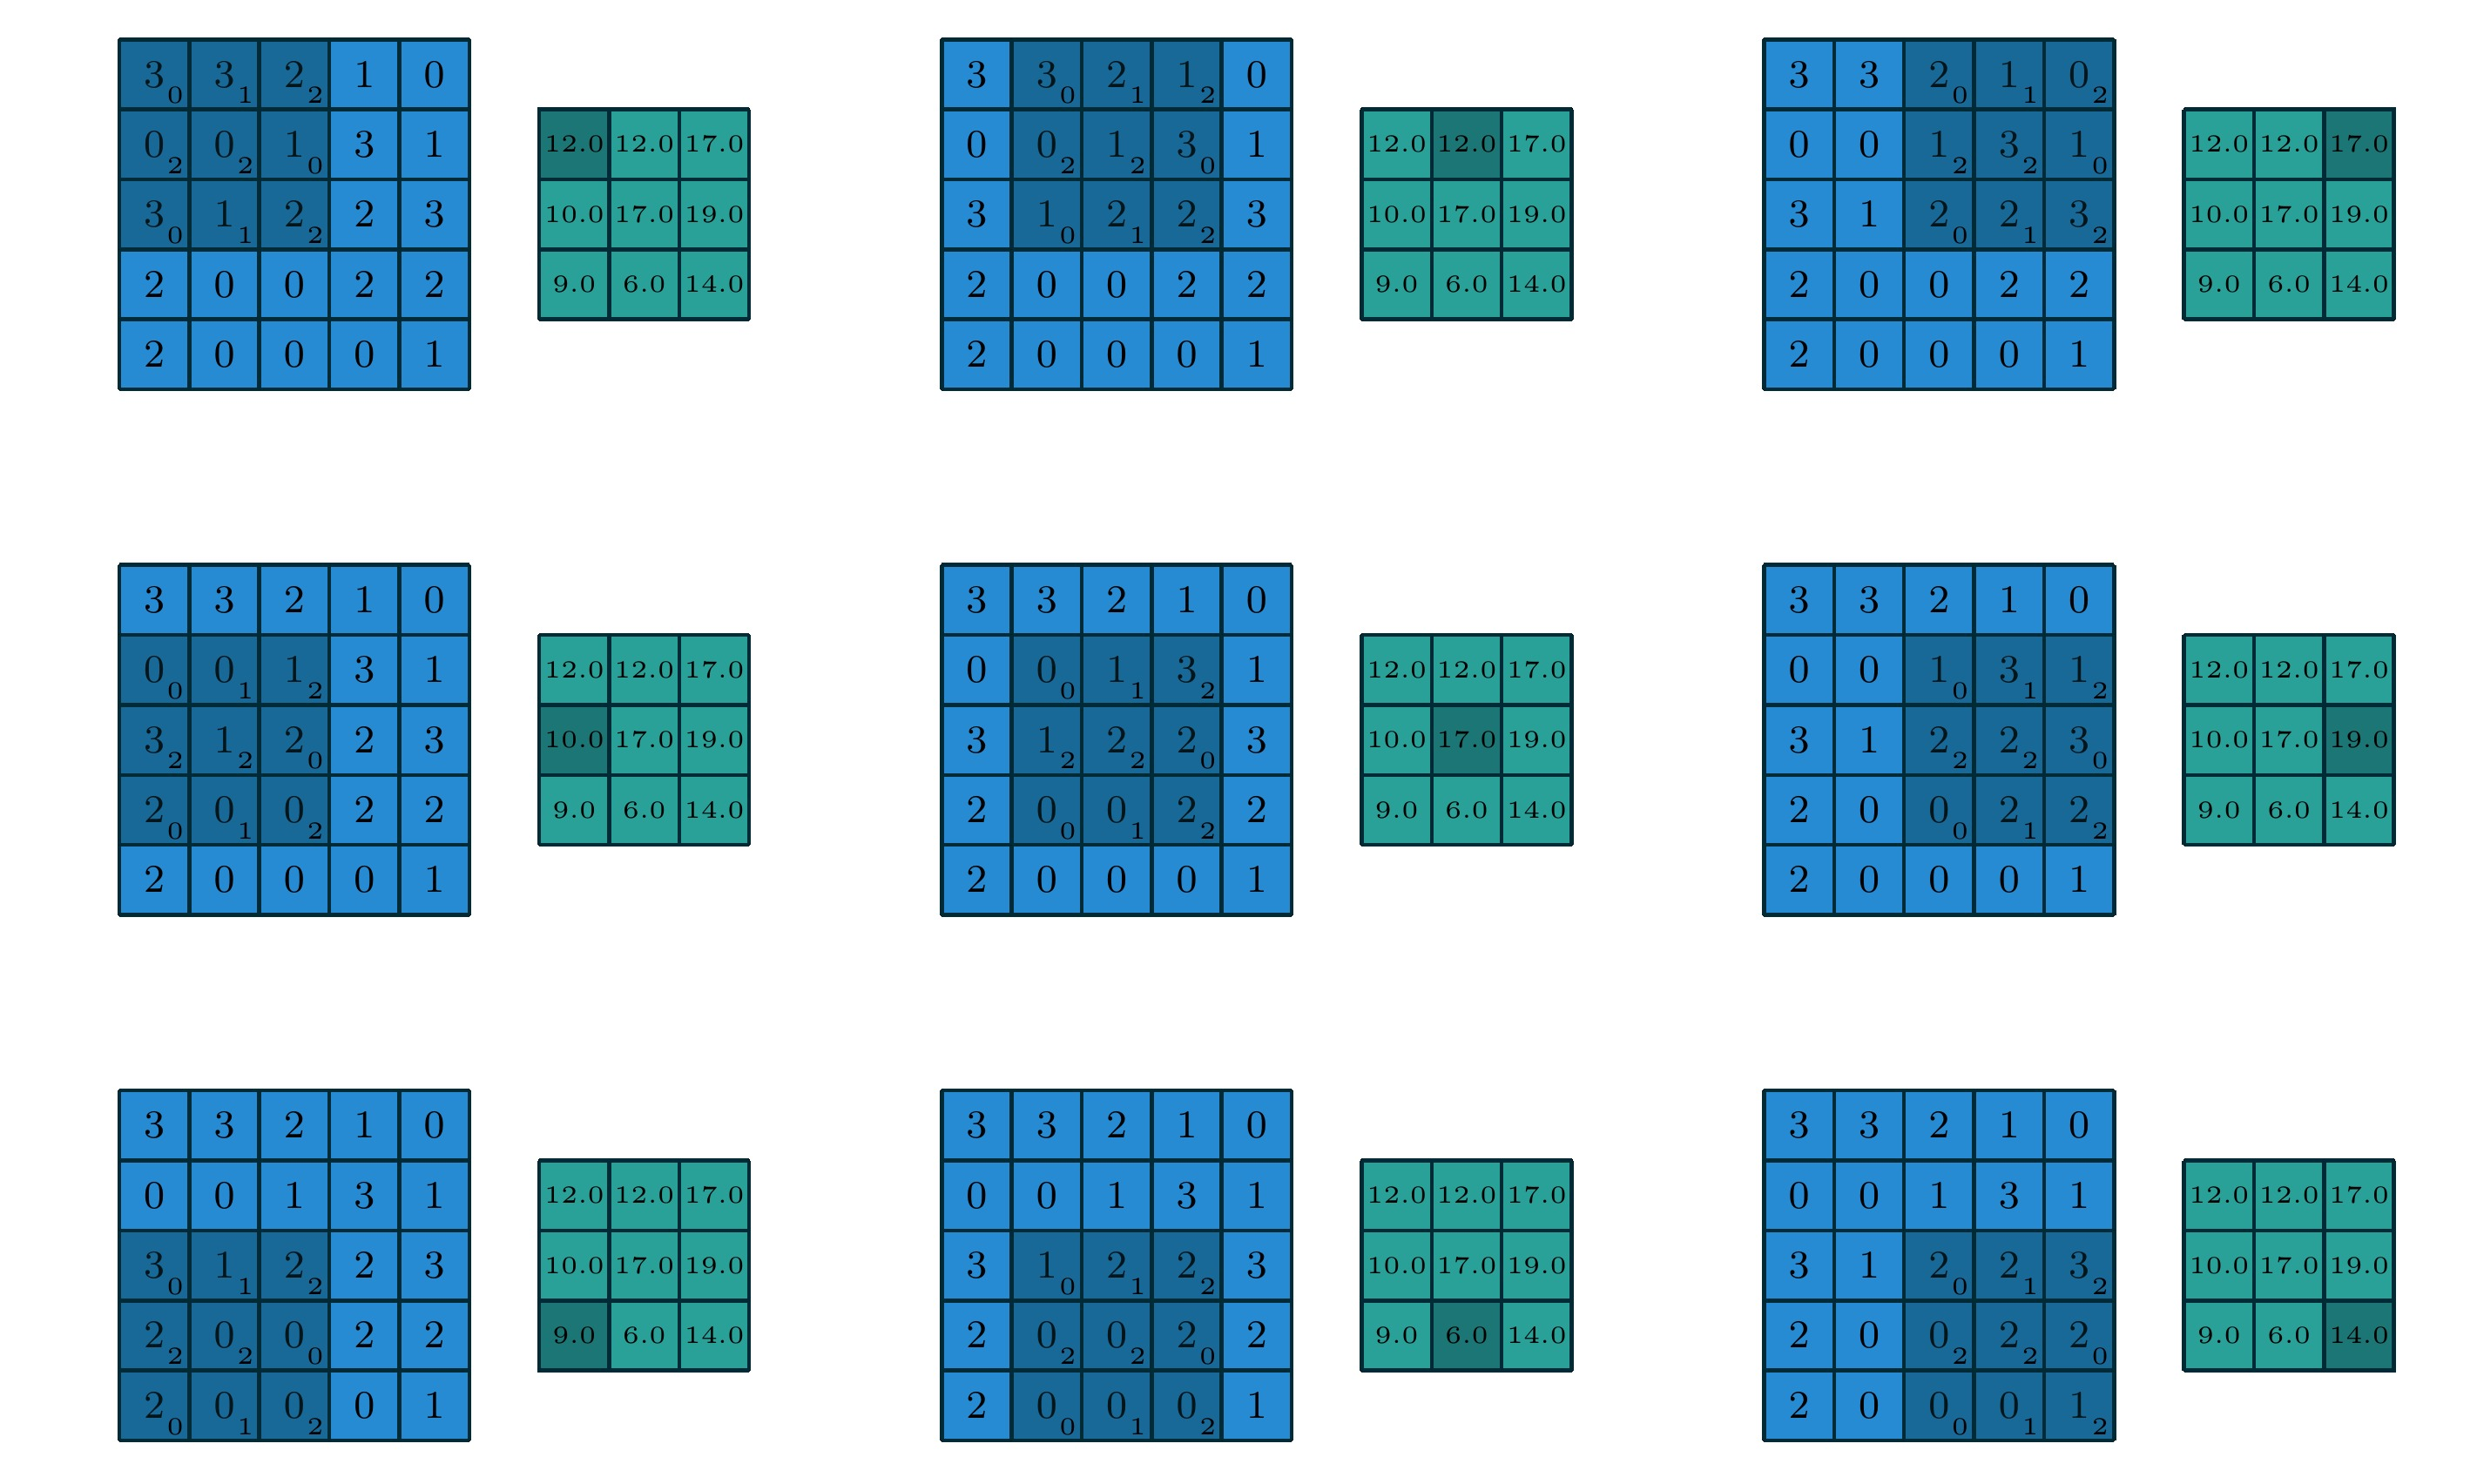
\includegraphics[width=1\textwidth]{images/convolucion/ima11.jpg}
    \caption{Muestra de la convolución aritmética en 2 dimensiones}
    \label{fig:convolucionArimetica}
\end{figure}

        
        En el caso practico más sencillo, el valor de la salida de esta operación con una entrada de dimensiones ($N, C_{in}, H, W$) y de una salida de dimensiones ($N, C_{out}, H_{out}, W_{out}$)  esta descrito por la siguiente fórmula:
\begin{equation}
    out(N_i, C_{out_j})=bias(Cout_j)+\sum_{k=0}^{C_{in}-1}weight(C_{out_j},k)\star input(N_i, k)
\end{equation}

Donde $\star$ es el operador de convolución que fue descrito en la sección \ref{subsec:convolucion}, N es el tamaño de \gls{Batch}, C denota el numero de canales, H es la altura de las entradas, y W es el ancho.

Las convoluciones tienen los siguientes parámetros de configuración:
\begin{itemize}
    \item \textbf{\gls{Stride}} controla la separación entre cada paso de la convolución .
    \begin{figure}[H]
    \centering
    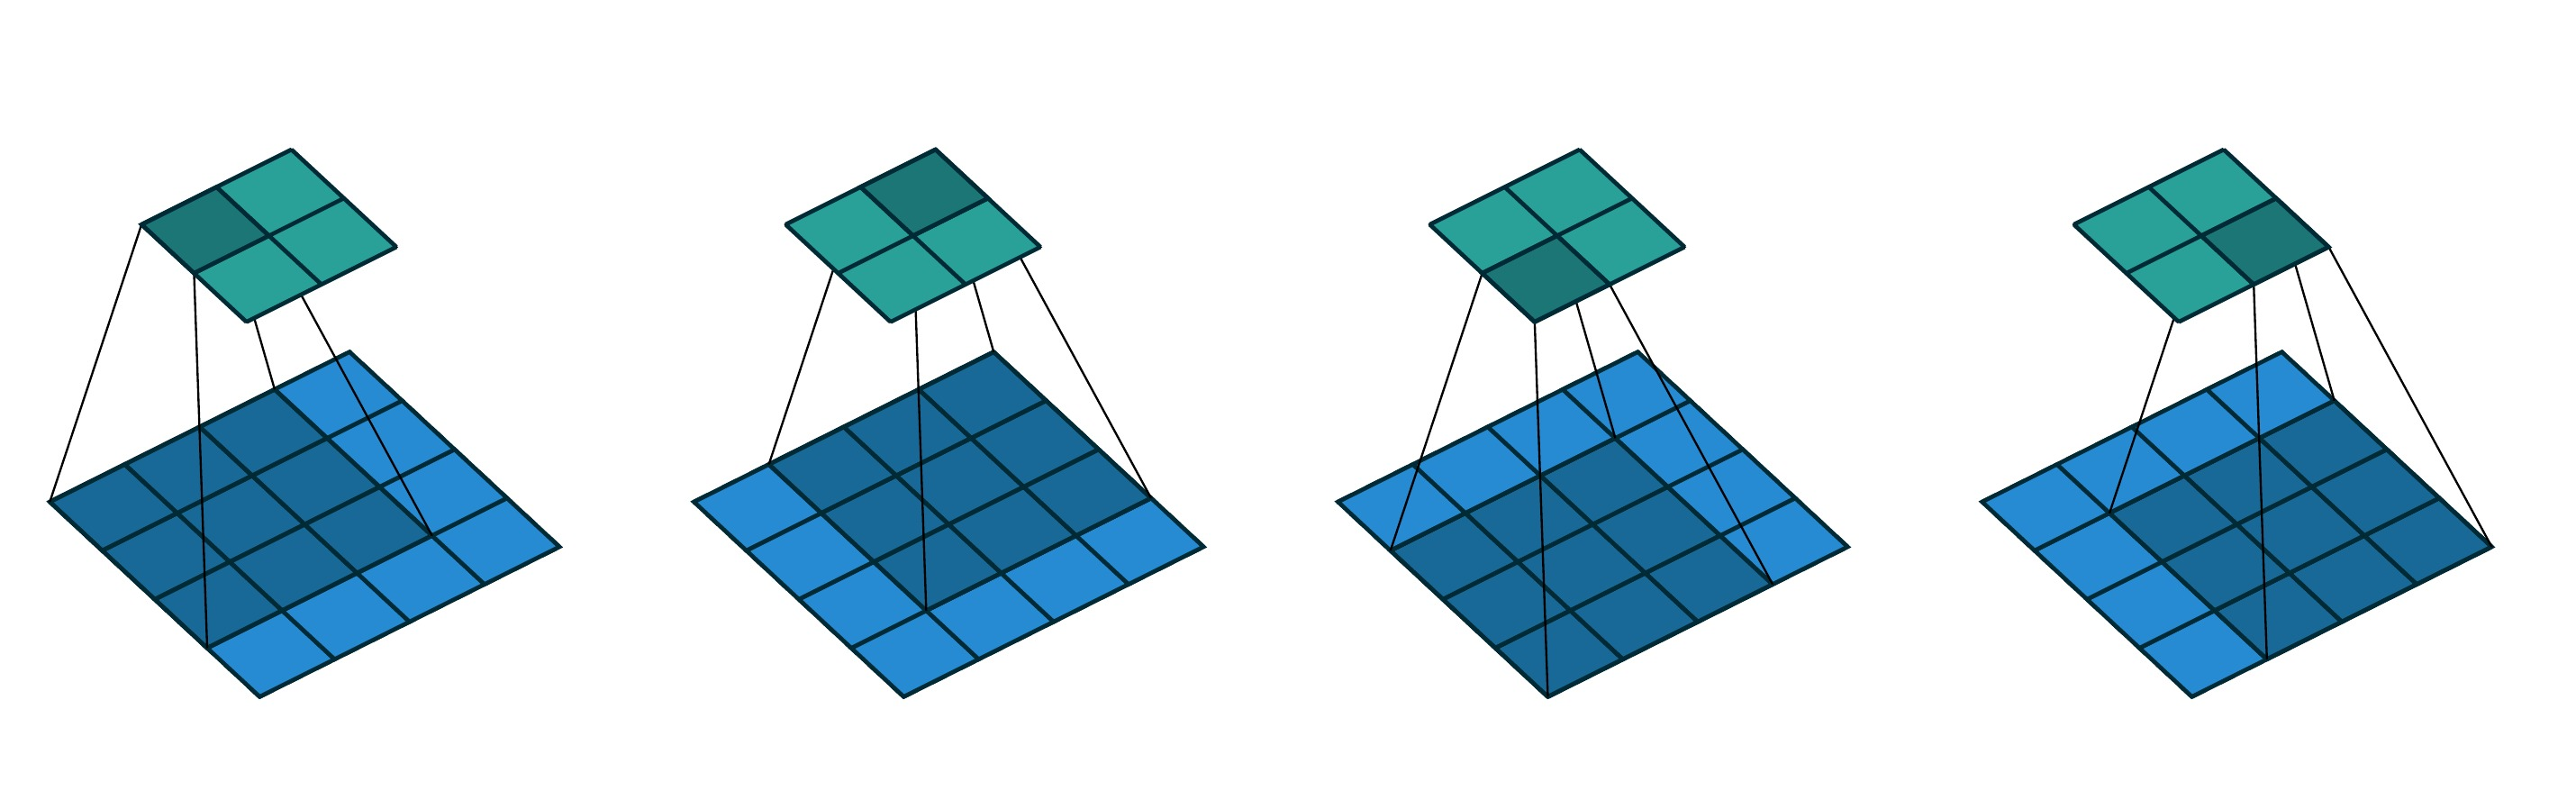
\includegraphics[width =0.9\textwidth]{images/convolucion/ima21.jpg}
    \caption{Operación de convolución con el \gls{Stride} de tamaño 1 sin padding}
    \label{fig:my_label}
\end{figure}
\begin{figure}[H]
    \centering
    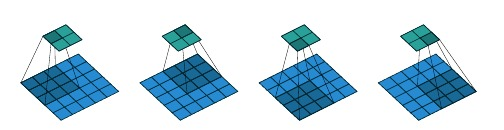
\includegraphics[width =0.9\textwidth]{images/convolucion/ima25.jpg}
    \caption{Operación de convolución con el \gls{Stride} de tamaño 2 sin padding}
    \label{fig:my_label}
\end{figure}
    \item \textbf{Padding} controla la cantidad de zeros agregados en ambos lados.
    
\begin{figure}[H]
    \centering
    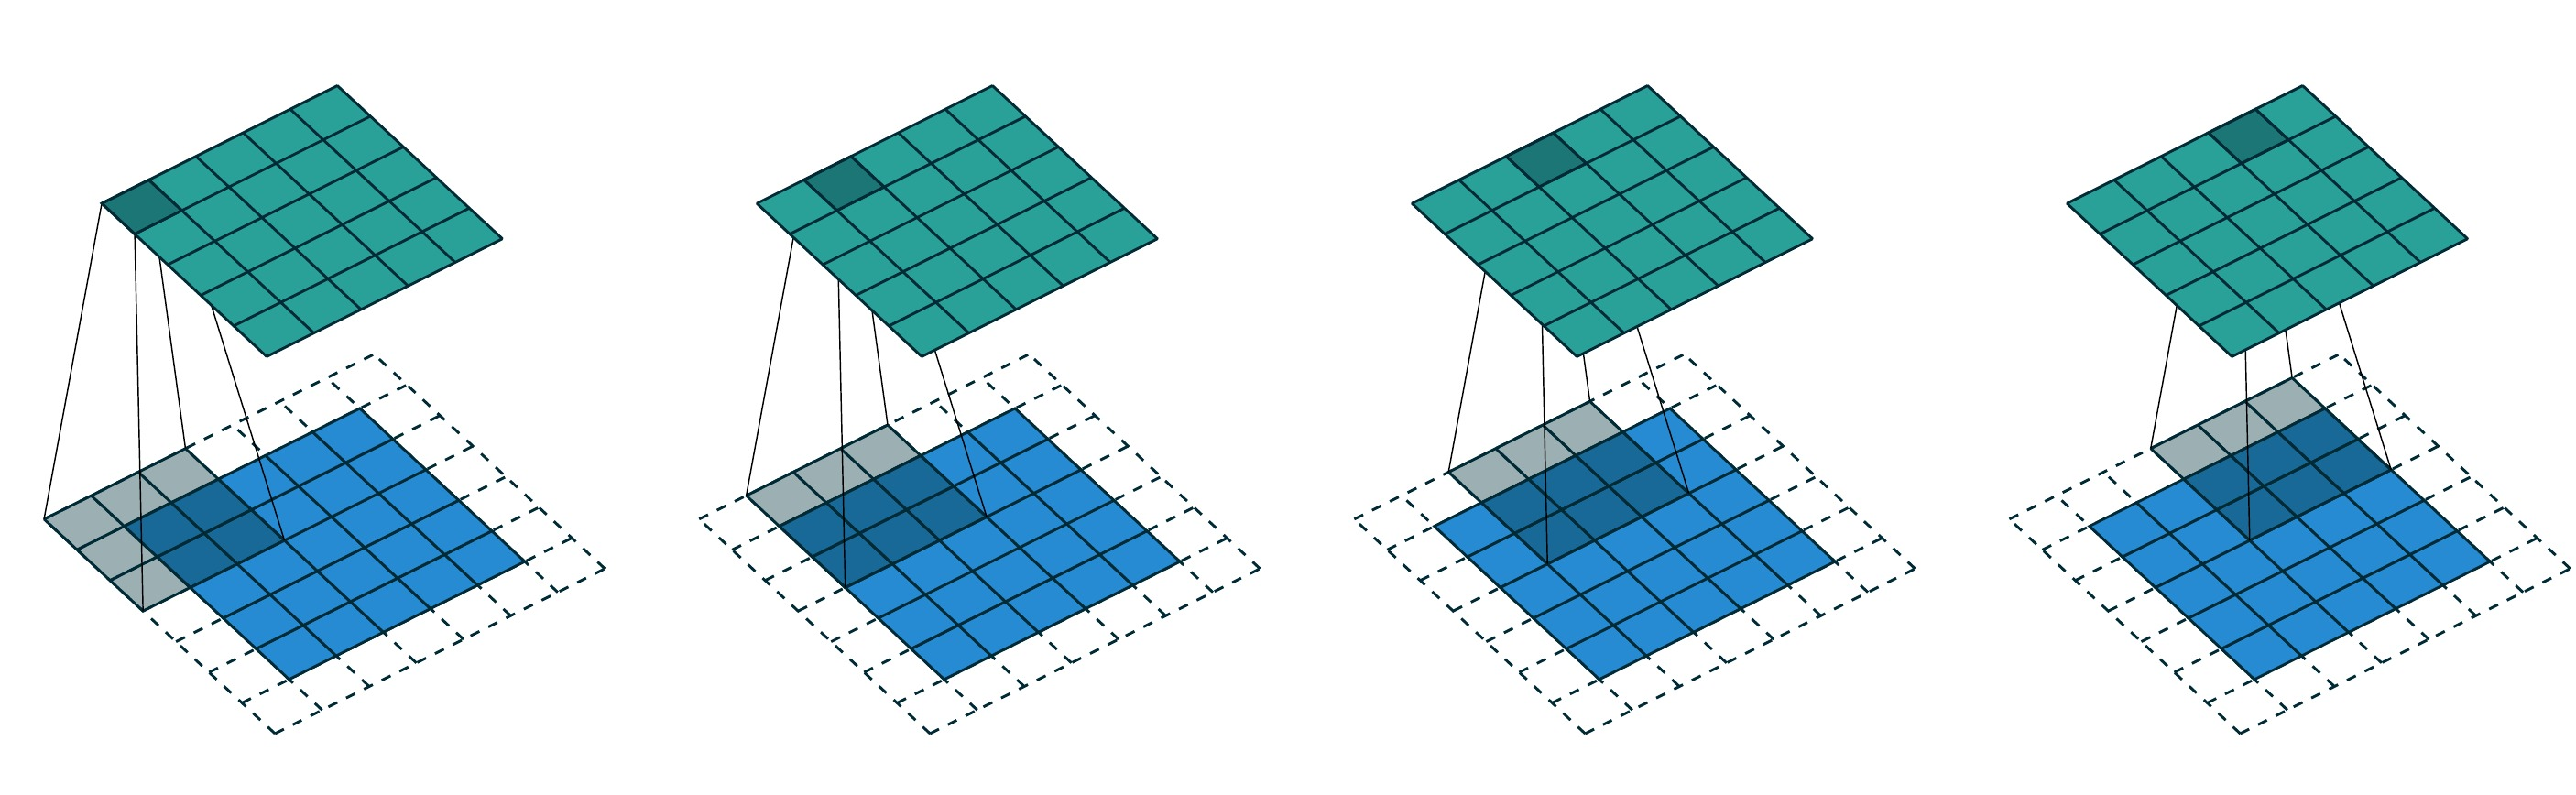
\includegraphics[width =0.9\textwidth]{images/convolucion/ima23.jpg}
    \caption{Operación de convolución con Padding de 1, \gls{Stride} de 1  }
    \label{fig:my_label}
\end{figure}
\begin{figure}[H]
    \centering
    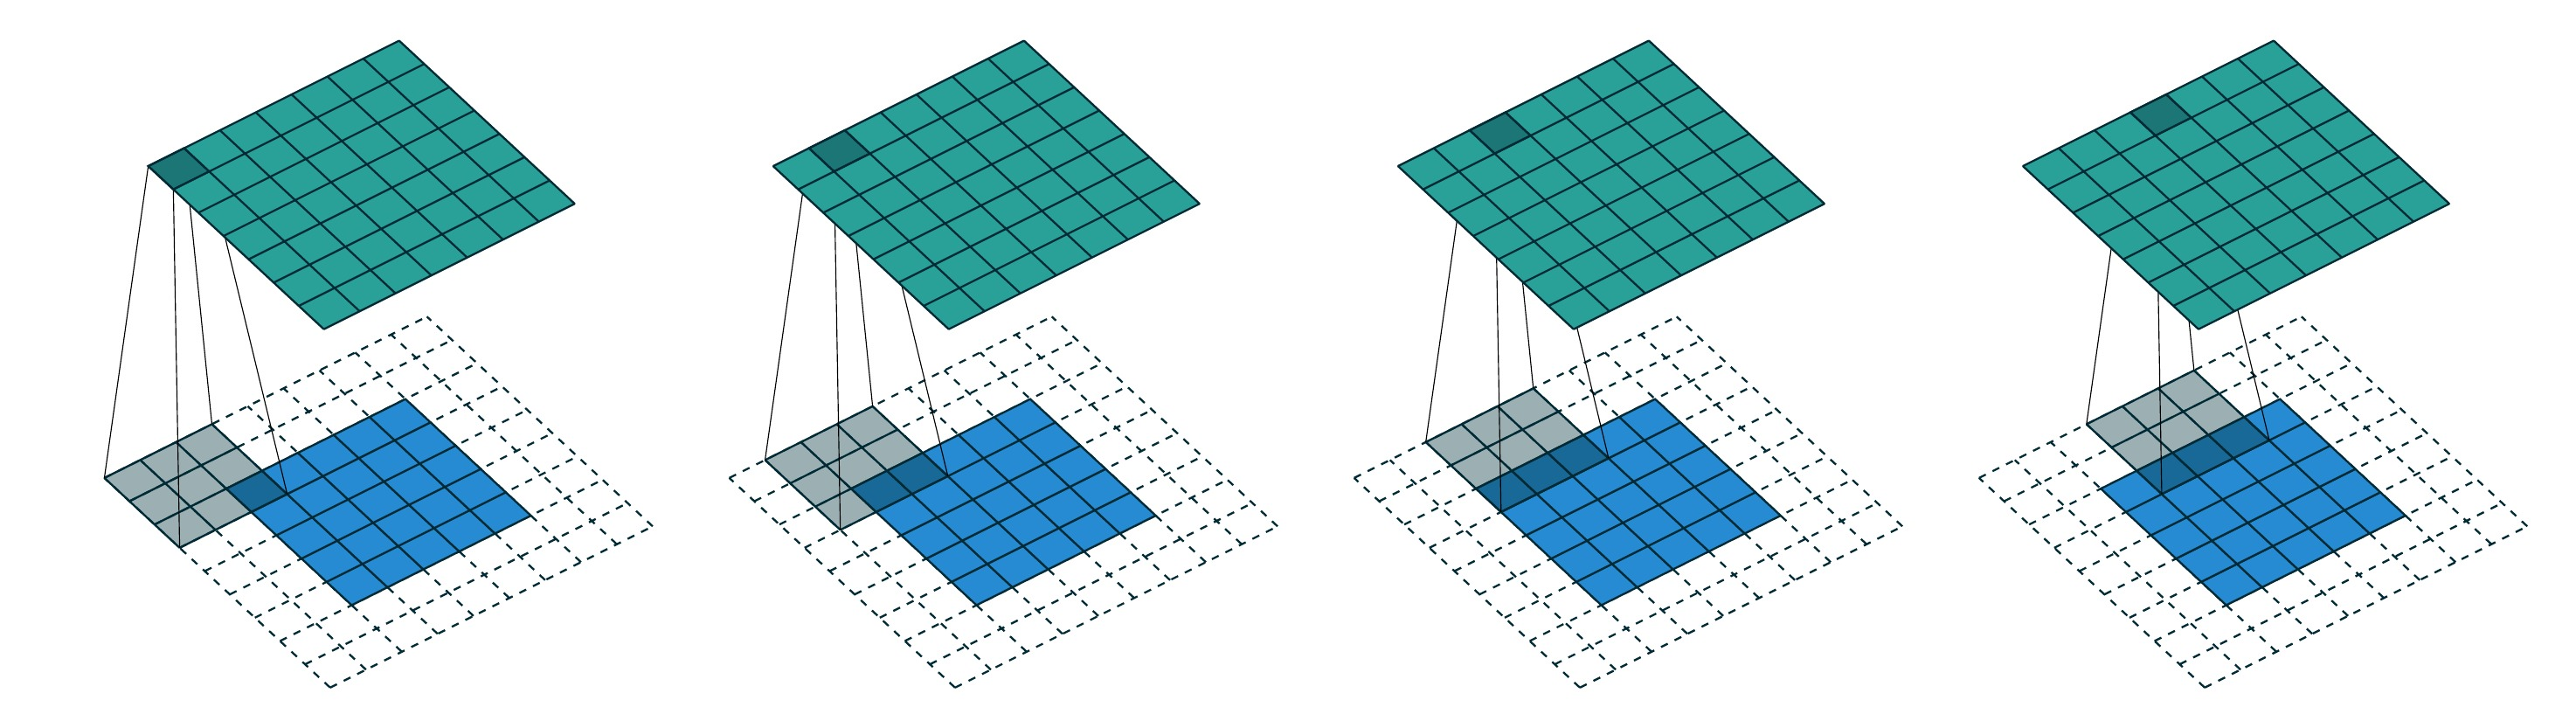
\includegraphics[width =0.9\textwidth]{images/convolucion/ima24.jpg}
    \caption{Operación de convolución con Padding de 2, \gls{Stride} de 1  }
    \label{fig:convolucionNormal}
\end{figure}

\begin{figure}[H]
    \centering
    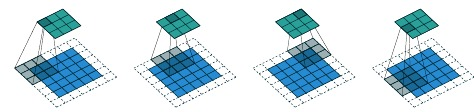
\includegraphics[width =0.9\textwidth]{images/convolucion/ima26.jpg}
    \caption{Operación de convolución con Padding de 2, \gls{Stride} de 2}
    \label{fig:my_label}
\end{figure}
    \item \textbf{Dilation} controla el espacio entre los puntos del \gls{kernel} como se ve en la \figurename~\ref{fig:dilatation}
    
\begin{figure}[H]
    \centering
    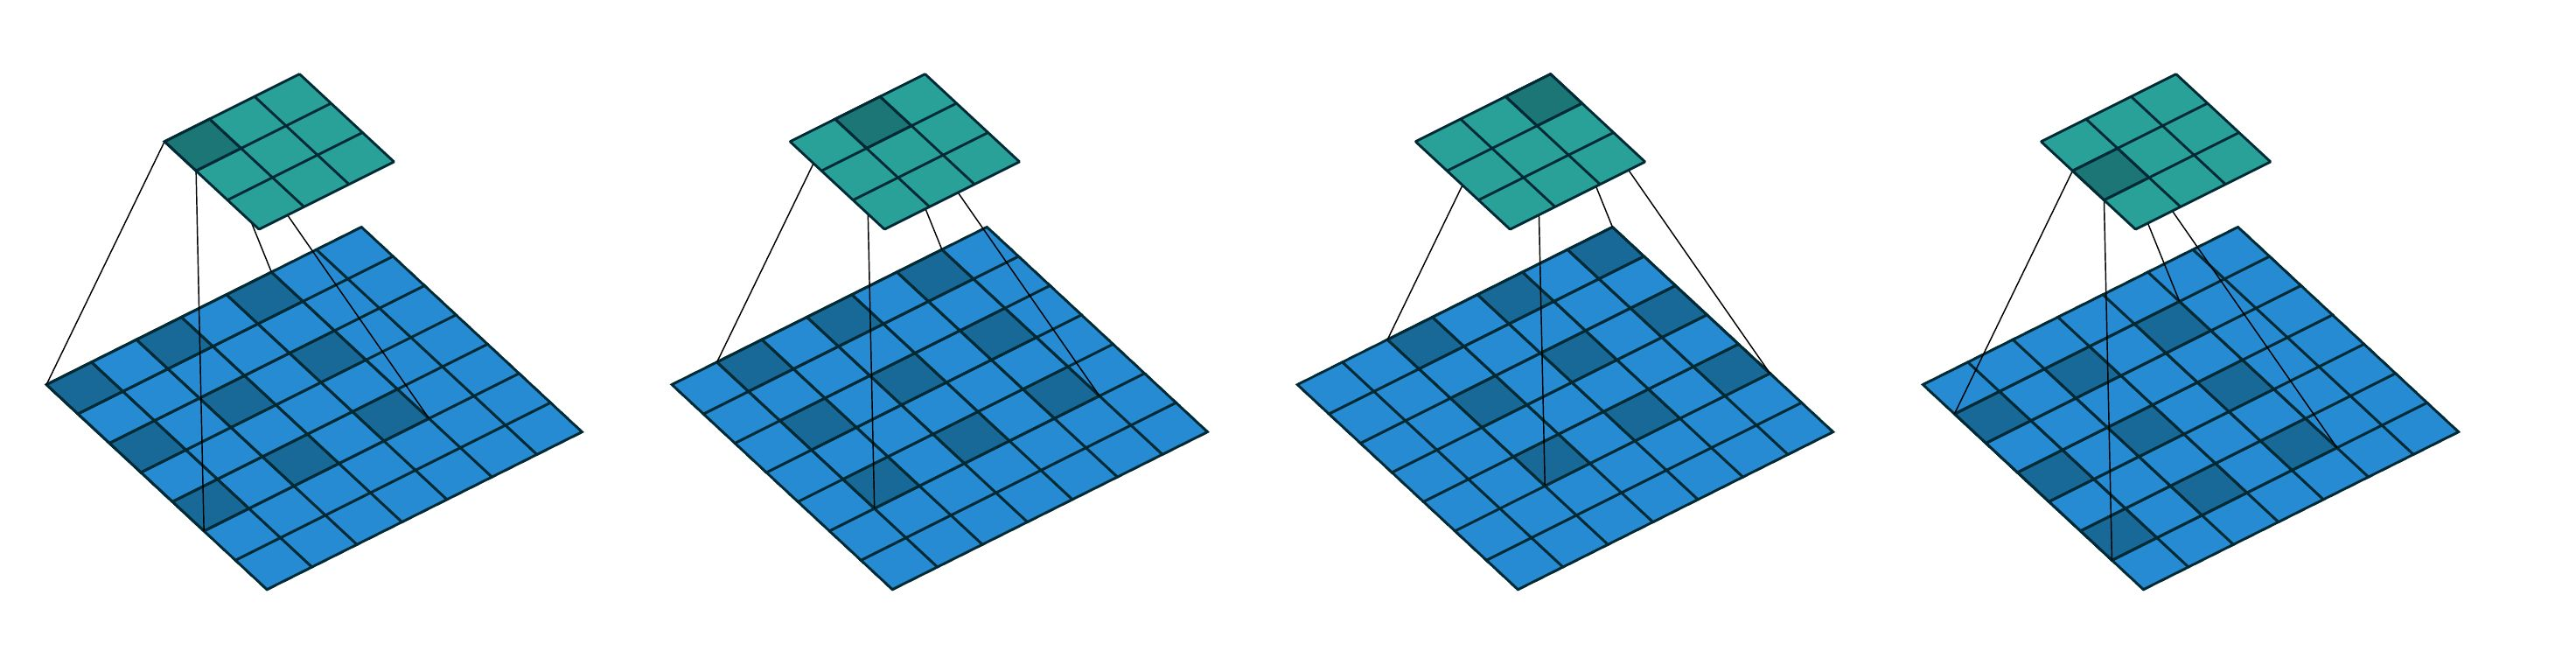
\includegraphics[width =0.9\textwidth]{images/convolucion/ima51.jpg}
    \caption{Convolución dilatada}
    \label{fig:dilatation}
\end{figure}
 
    \item \textbf{Groups} controla las conecciones entre la entrada y la salida -
            \begin{itemize}
                \item Si groups=1, todos las entradas son convolucionadas para todas las salidas.

            \item Si groups=2, la operación se convierte equivalente a tener 2 \gls{Layer}s convolucionales, cada uno ve la mitad de los canales de entrada, y produce la mitad de los canales de salida y ambos concatenados.

            \item Si groups= in\_channels, cada canal es convolucionado con su propio filtro, de tamaño: $\frac{out\_Channel}{in\_Channel}$
            \end{itemize}
            
 \begin{figure}[H]
\begin{subfigure}{.33\textwidth}
  \centering
    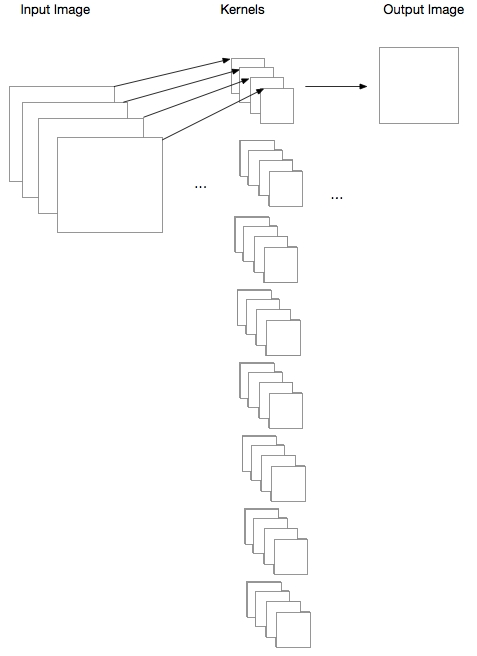
\includegraphics[width =0.9\textwidth]{images/group/g1.jpg}
  \caption{Grupo = 1}
  \label{fig:sfig1}
\end{subfigure}%
\begin{subfigure}{.33\textwidth}
  \centering
        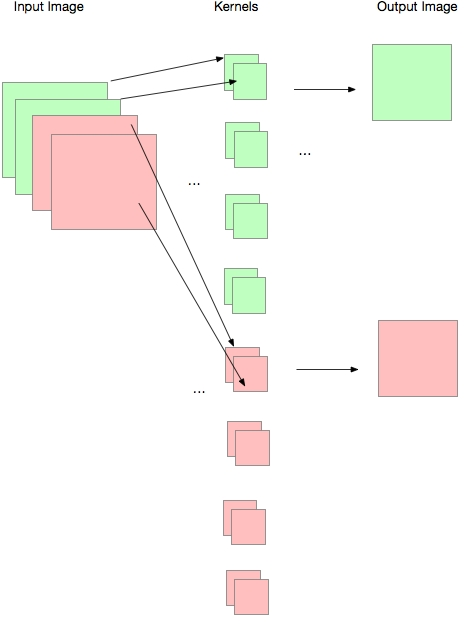
\includegraphics[width =0.9\textwidth]{images/group/g2.jpg}
  \caption{Grupo = 2}
  \label{fig:sfig2}
\end{subfigure}
\begin{subfigure}{.33\textwidth}
  \centering
    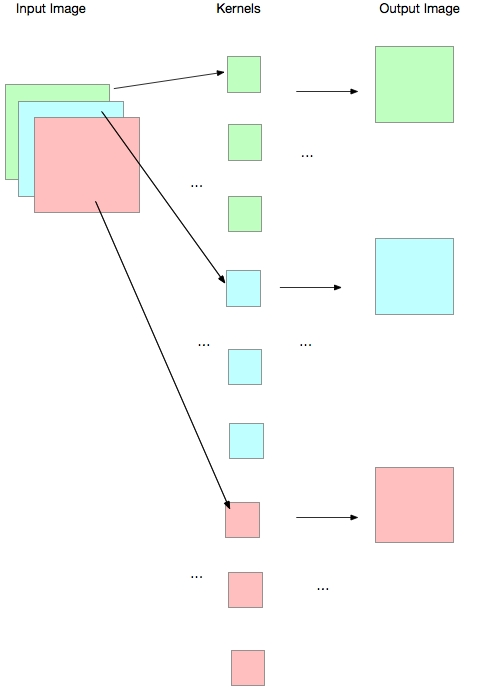
\includegraphics[width =0.9\textwidth]{images/group/g3.jpg}
  \caption{Grupo = 3}
  \label{fig:sfig2}
\end{subfigure}
\caption{Distintos tamaños de grupo}
\label{fig:convolucionGrupos}
\end{figure}
\end{itemize}
    
A continuación se pueden ver las dimensiones:
\begin{itemize}
    \item Entrada: (N, $C_{in}$, $H_{in}$, $W_{in}$)

    \item    Salida: (N, $C_{out}$, $H_{out}$, $W_{out}$) donde
       
        \begin{equation}
            H_{out}= \frac{H_{int}+2\times padding[0]-dilation[0]\times (\gls{kernel}\_ size[0]-1)-1}{\gls{Stride}[0]} 
        \end{equation}
        \begin{equation}
            W_{out}= \frac{W_{int}+2\times padding[1]-dilation[1]\times (\gls{kernel}\_ size[1]-1)-1}{\gls{Stride}[1]} 
        \end{equation}
 
\end{itemize}

\subsubsection{Pooling }
En adición a las convoluciones discretas, las operaciones de \gls{Pooling} son importante para la construcción de \gls{CNN}s. Las operaciones de \gls{Pooling} reduce el tamaño de los mapas de características usando funciones que resumen subregiones, como es el tomar el promedio o el máximo valor. 

\gls{Pooling} trabajo deslizando una ventana por la entrada y sometiendo el contenido de la ventana a una función de \gls{Pooling}. En algún sentido, el \gls{Pooling} funciona como una convolución discreta, pero reemplaza la combinación linear con otra función. La \figurename~\ref{fig:poolAverage} muestra un ejemplo de \gls{Pooling} por promedio, y la \figurename~\ref{fig:poolMax} muestra un ejemplo de \gls{Pooling} máximo.

Las siguientes propiedades afectan el tamaño de la salida $o$ de un \gls{Layer} de \gls{Pooling} 
\begin{itemize}
    \item $i$ : El tamaño de la entrada,
    \item $k$ : El tamaño de la ventana,
    \item $s$ : La distancia entre 2 ventanas consecutivas.
 
\end{itemize}
\begin{equation}
    o = \lfloor\frac{i-k}{s}\rfloor+1
\end{equation}
El tipo más común de agrupación es la agrupación máxima, que consiste en dividir el valor de entrada en cada uno de los valores de parche y cada uno de los valores de parche. Existen tipos de agrupación, por ejemplo, agrupación media o promedio, que comparten la misma idea de agregar la entrada localmente aplicando una no linealidad al contenido de algunos parches~\cite{boureau2010learning}.


\begin{figure}[H]
    \centering
    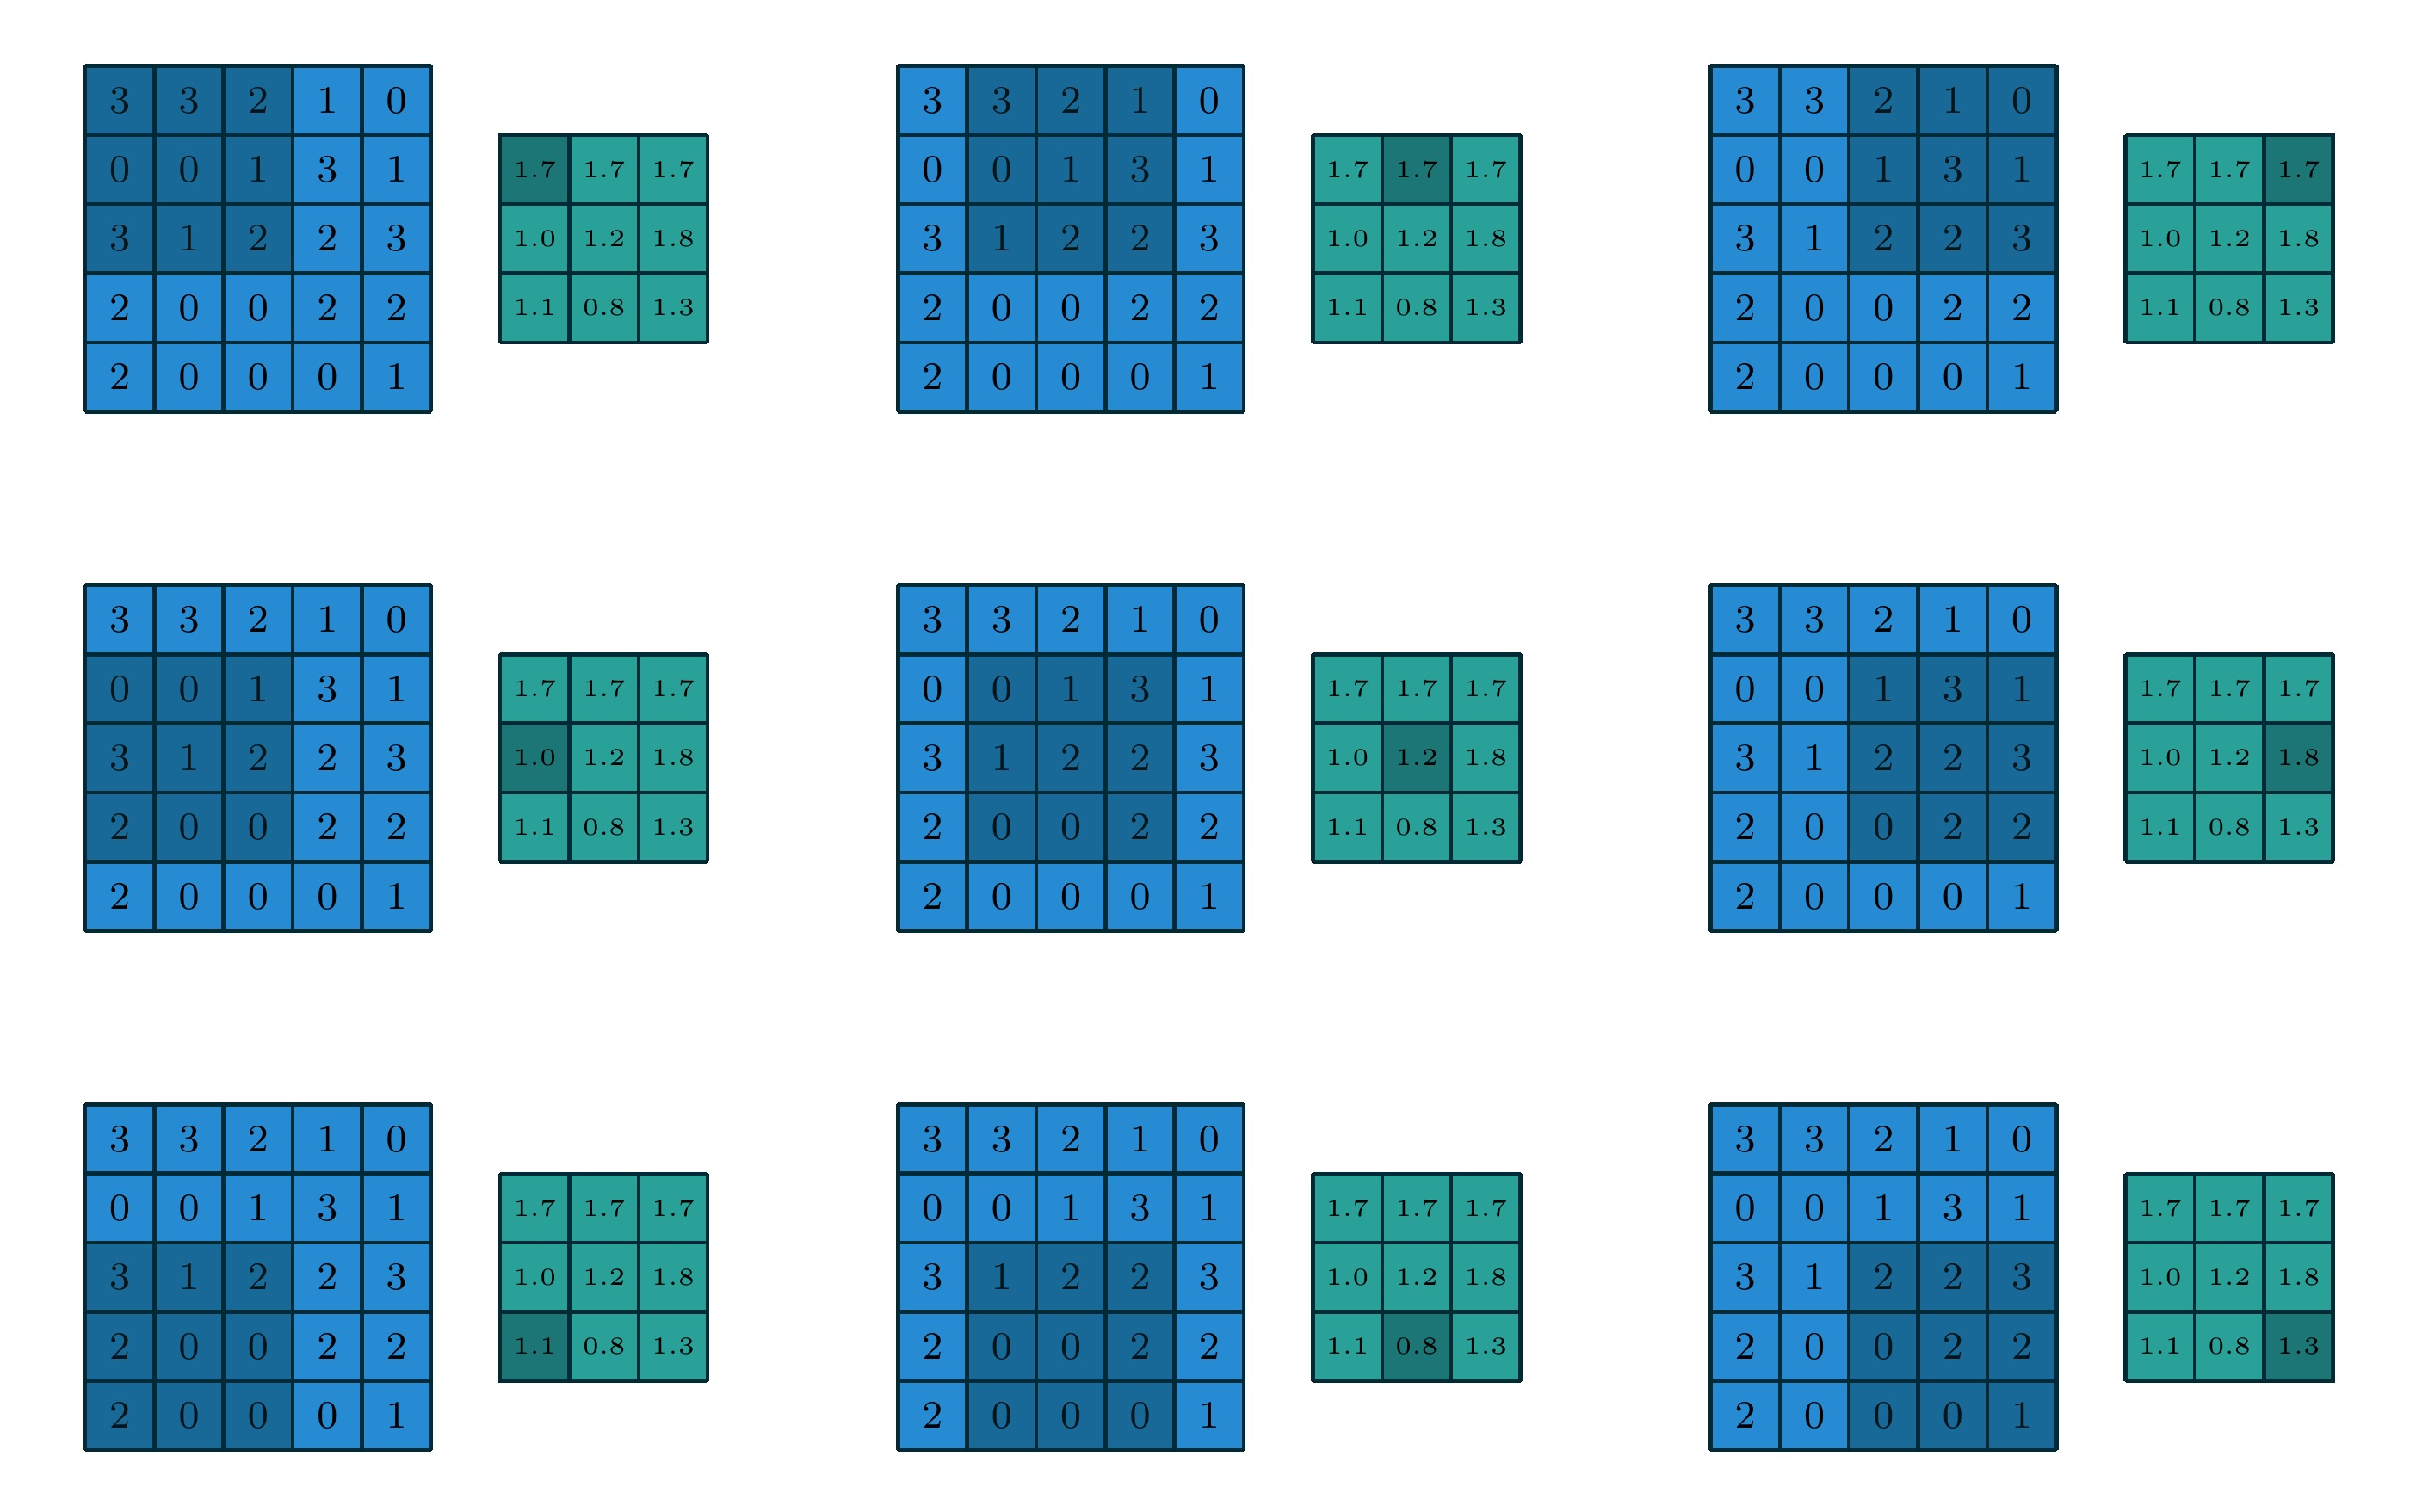
\includegraphics[width =0.9\textwidth]{images/convolucion/ima15.jpg}
    \caption{\gls{Pooling} por promedio}
    \label{fig:poolMax}
\end{figure}
\begin{figure}[H]
    \centering
    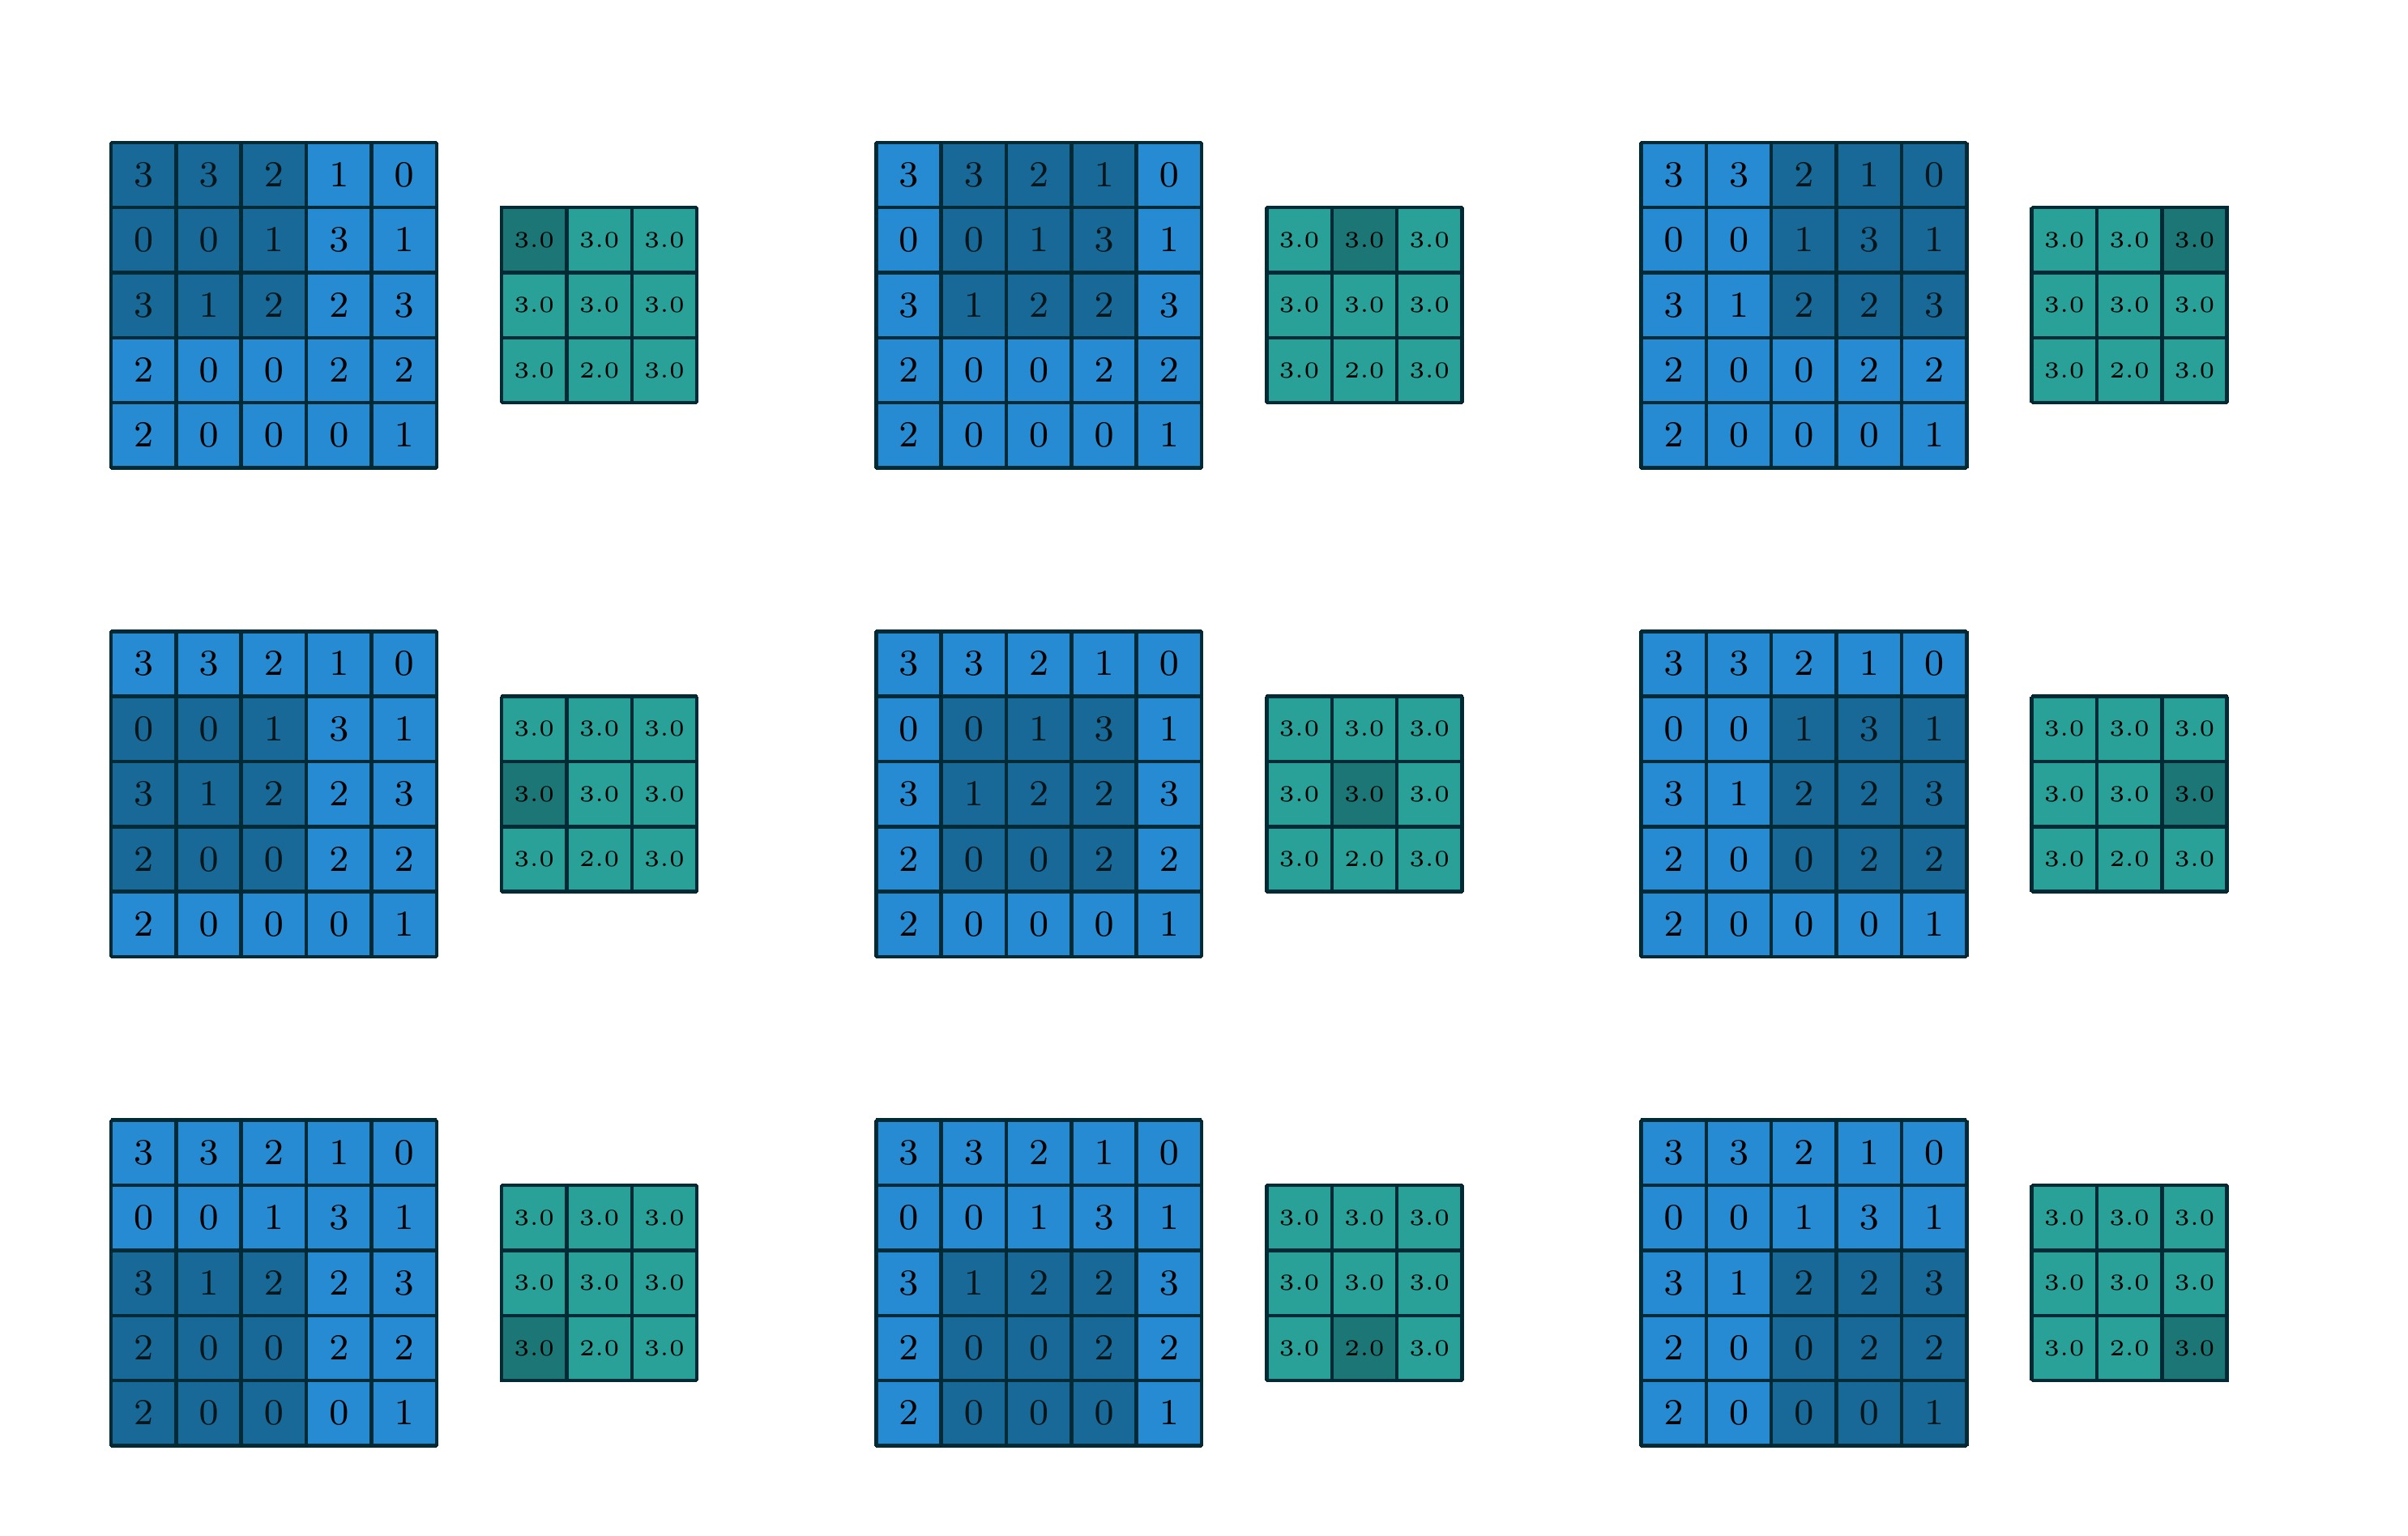
\includegraphics[width =0.9\textwidth]{images/convolucion/ima16.jpg}
    \caption{\gls{Pooling} por valor máximo}
    \label{fig:poolAverage}
\end{figure}

El valor de la salida de esta operaciones cuya entrada es de tamaño (N, C, H, W), salida = N, C, $H_{out}$, $W_{out}$ y de tamaño de \gls{kernel} $kH$, $kW$ puede ser descrito por la siguiente fórmula
\begin{equation}
\begin{split}
    out(N_i,C_J,h,w)=  &\max_{m=0 ,..., kH-1}\max_{n=0 ,...,kW-1}    \\
    &input(N_i,C_j,\gls{Stride}[0]\times h+m,\gls{Stride}[1]\times w+n)
\end{split}
\end{equation}

El \gls{Pooling} puede presentar los siguientes parámetros 
\begin{itemize}
    \item  \textbf{Tamaño de \gls{kernel}:} El tamaño de la ventana

    \item    \textbf{Stride:} El desplazamiento de la ventana, lo normal es que este sea del tamaño del \gls{kernel}.

    \item    \textbf{Padding:} Valores de zero agregado en los bordes.

    \item    \textbf{Dilation:} Controla la separación entre los cuadros de la ventana, se aprecia en la \figurename~\ref{fig:dilatation}
    
\end{itemize}{}

        


De lo anterior se obtienen las siguientes dimensiones:
        Input: (N, C, $H_{in}$, $W_{in}$)
        
        Output: (N, C, $H_{out}$, $W_{out}$) donde
        
        
        \begin{equation}
         H_{out}= \frac{H_{in}+2\times padding[0]-dilation[0]\times (\gls{kernel}\_size[0]-1)-1}{stride[0]} +1  
        \end{equation}
        \begin{equation}
         W_{out}= \frac{W_{in}+2\times padding[1]-dilation[1]\times (\gls{kernel}\_size[1]-1)-1}{stride[1]} +1  
        \end{equation}
        



\subsubsection{Convolución Transpuesta}
\label{sub:convolucionTranspuesta}
La necesidad de la convolución transpuesta generalmente llega a partir del deseo de usar una transformación en la dirección opuesta de la convolución normal, por ejemplo si deseamos obtener el tamaño de la entrada mientras se mantiene un patrón de conectividad. Esta operación es usada en lo decodificadores y el upsampling de varias redes neuronales.

Como por ejemplo en la \figurename~\ref{fig:convolucionNormal}. Si la entrada y la salida fueran desenrollados en vectores de izquierda a derecha, de arriba a abajo, la convolución podría ser representada como una matriz dispersa donde los elementos que no sean zeros son los elemento w, i, j del \gls{kernel} donde i y j es la fila y la columna respectivamente

\setcounter{MaxMatrixCols}{20}
\begin{figure}[H]

\begin{adjustbox}{max width=\textwidth}
\begin{bmatrix}
W_{0,0} & W_{0,1} & W_{0,2} & 0 & W_{1,0} & W_{1,1} & W_{1,2}& 0 & W_{2,0} & W_{2,1} & W_{2,2} & 0 & 0 & 0 &  0 & 0 \\
0 & W_{0,0} & W_{0,1} & W_{0,2} & 0 & W_{1,0} & W_{1,1} & W_{1,2}& 0 &W_{2,0} & W_{2,1} & W_{2,2}& 0 & 0 & 0&  0 \\
0 & 0 & 0&  0 & W_{0,0} & W_{0,1} & W_{0,2} & 0 & W_{1,0} & W_{1,1} & W_{1,2}& 0 &W_{2,0} & W_{2,1} & W_{2,2}&  0 \\
0 & 0 & 0 &  0 & 0 & W_{0,0} & W_{0,1} & W_{0,2} & 0 & W_{1,0} & W_{1,1} & W_{1,2}& 0 &W_{2,0} & W_{2,1} & W_{2,2}
\end{bmatrix}
\end{adjustbox}

\caption{Matriz C que representa la operación de convolución de la \figurename~\ref{fig:convolucionNormal}}
\label{fig:convolucionComoMatriz}
\end{figure}{}
Esta operación lineal toma la entrada de la matriz aplanada como un vector de 16 dimensiones y produce un vector de 4 dimensiones que es después es reconstruido a una matriz de 2 por 2.  Usando esta representación, el paso contrario puede ser obtenido fácilmente al transponer la matriz $C$, en otras palabras, el error es retropropagado por multiplicar la perdida con $C^T$. Esta operación toma un arreglo de dimensión 4 como entrada y produce y arreglo de 16 dimensiones como salida. Es notable que el \gls{kernel} w define ambas matrices $C$ y $C^T$

La Convolución Transpuesta llamada(también fractionally strided o deconvolución\footnote{El termino deconvolución aveces es usado en la literatura, pero no esta del todo bien utilizado debido a que en matemática la deconvolución es la operación inversa de la convolución}) funciona invirtiendo los pasos de forward y backward de una convolución. Es notorio que el \gls{kernel} define una convolución directa o una convolución transpuesta pero el determinar si es una u otra depende de como se computa el forward y el backward. Por ejemplo, aunque el \gls{kernel} w define una convolución cuyos pasos de forward and backward son computados por la multiplicación de $C^T$ y $(C^T)^T=C$ respectivamente\footnote{La convolución transpuesta puede ser pensada como la gradiente de alguna convolución con respecto a la entrada, que es de hecho como las convoluciones transpuestas son implementadas en practica}

\begin{figure}[H]
    \centering
    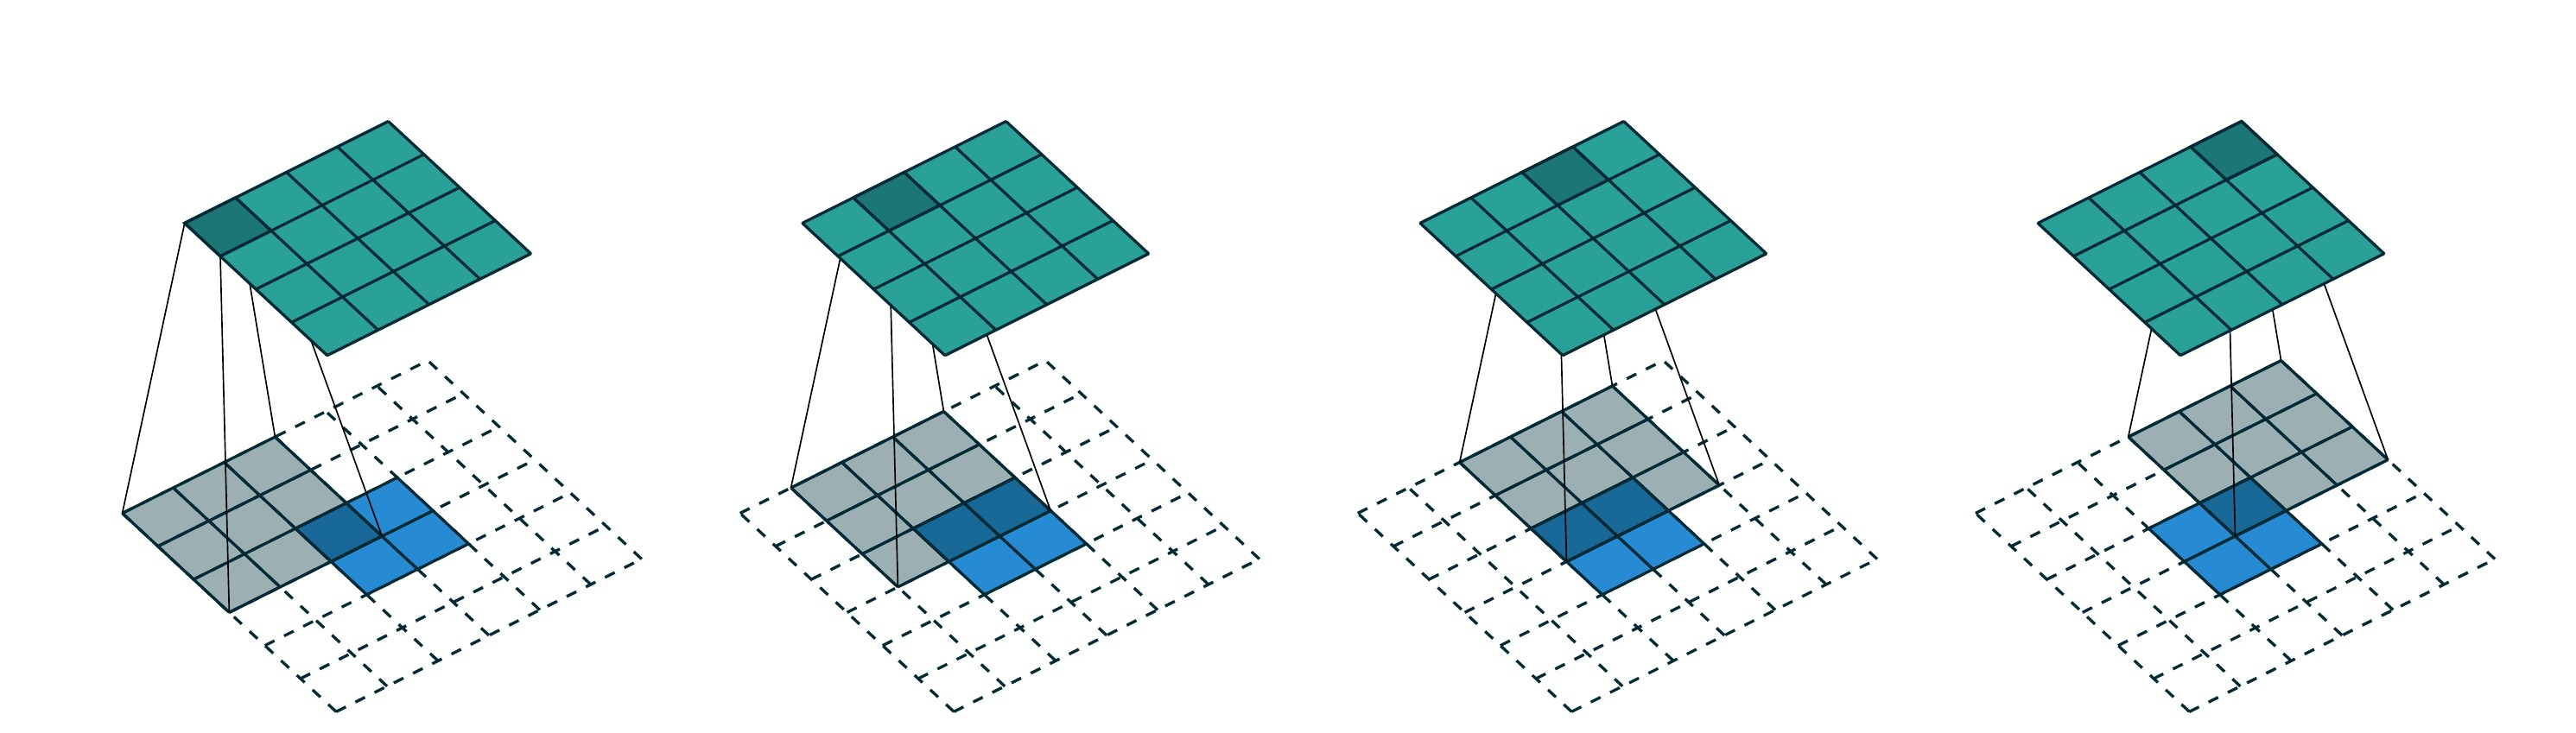
\includegraphics[width =0.9\textwidth]{images/convolucion/ima41.jpg}
    \caption{Muestra de convolución transpuesta}
    \label{fig:my_label}
\end{figure}
Los parámetros manejados para la convolución transpuesta son 
\begin{itemize}
    \item   \textbf{Stride} controla el desplazamiento del \gls{kernel}.

    \item \textbf{Padding} controla la cantidad de zeros en los bordes.

    \item \textbf{Output\_padding} Controla la cantidad de zeros agregados en la salida.

    \item \textbf{Dilation} controla el espacio entre los elementos del \gls{kernel}\ref{fig:dilatation}.

    \item \textbf{Groups} controla las conexiones entre la entrada y la salida, se aprecia mejor en la \figurename~\ref{fig:convolucionGrupos}
    \begin{itemize}
        \item  Con groups=1, todos los elementos de la entrada se convolución en los de la salida.

        \item    Con groups=2, la operación se vuelve equivalente a tener 2 capas, cada uno viendo solo la mitad de los canales de entrada .

     

    \end{itemize}
            
\end{itemize}
   
De lo anterior mencionado se puede calcular lo siguiente.
        Input: (N, $C_{in}$, $H_{in}$, $W_{in}$)
        Output: (N, $C_{out}$, $H_{out}$, $W_{out}$) donde

        
        \begin{equation}
            H_{out} = \frac{H{in}+2\times padding[0]-dilation[0]\times (\gls{kernel}\_size[0]-1)-1}{stride[0]} +1
        \end{equation}
         
        \begin{equation}
            W_{out} = \frac{W{in}+2\times padding[1]-dilation[1]  \times (\gls{kernel}\_size[1]-1)-1}{stride[1]} +1
        \end{equation}
        
    Siendo N el tamaño de \gls{Batch} , $C_{in}$ y $C_{out}$ la cantidad de canales de entrada y salida respectivamente, $H_{in}$ y $H_{out}$ la altura de la entrada y salida respectivamente , $W_{in}$ y $W_{out}$ el ancho de la entrada y salida respectivamente.



    
\subsubsection{DropOut}

Aleatoriamente convierte a zero un canal\footnote{ Un canal es un \gls{Feature Map} de 2 dimensiones}. Cada canal sera convertido a zero independientemente en cada llamada a forward con una probabilidad $p$, es usual usar la distribución de Bernolli. 

Como se describe en el artículo~\cite{Tompson2014}, si los pixeles adyacentes dentro de los mapas de características están fuertemente correlacionados (como suele ocurrir en las primeras capas convolucionales), entonces el Dropout no regularizará las activaciones y, de lo contrario, solo resultará en una disminución efectiva de la tasa de aprendizaje.


\subsubsection{Normalización por batches}
 Según~\cite{Ioffe2015} el entrenamiento en las redes neuronales profundas se complica por el hecho de que la distribución de las entradas de cada capa cambia durante el entrenamiento, a medida que cambian los parámetros de las capas anteriores. Esto ralentiza el entrenamiento al requerir tasas de aprendizaje más bajas y una cuidadosa inicialización de parámetros, y hace que sea extremadamente difícil entrenar Modelos con saturación no lineales. Nos referimos a este fenómeno como cambio de covariables internas y resolvemos el problema al normalizar las entradas de capa. El método propuesto por~\cite{Ioffe2015} se basa en hacer de la normalización una parte de la arquitectura del modelo y realizar la normalización para cada mini batch de entrenamiento. La normalización por lotes nos permite utilizar índices de aprendizaje mucho más altos y ser menos cuidadosos con la inicialización. También actúa como regulador, en algunos casos eliminando la necesidad de abandono. 
 \begin{equation}
     y = \frac{x-E[x]}{\sqrt{var[x]+\epsilon}}
 \end{equation}

Donde:
\begin{itemize}
    \item \textbf{y} es el valor esperado. 
    \item \textbf{x} es el mini \gls{Batch}.
    \item \textbf{E[x]} es el promedio.
    \item \textbf{var[x]} es la varianza.
\end{itemize}{}


\subsection{Frameworks de Desarrollo}
    \paragraph{Tensorflow:} Es una biblioteca para el aprendizaje automático de código abierto para investigación y producción utilizada para el cálculo numérico mediante diagramas de flujos de datos. Los nodos de los diagramas representan operaciones matemáticas y las aristas las matrices de datos multidimensionales (tensores) comunicadas entre ellas. Se necesita una API para desplegar el sistema informático de una o varias CPU o GPU. TensorFlow fue desarrollado por el ``Google Brain Team'' que formaban parte de la organización de investigación de aprendizaje automático de Google~\cite{Brain2015}.
   
    \paragraph{Keras:}Keras es una \gls{API} de redes neuronales de alto nivel para la construcción y entrenamiento de modelos de aprendizaje profundo, implementada en Python y capaz de ejecutarse sobre TensorFlow, CNTK o Theano. Fue desarrollado con el objetivo de permitir una experimentación rápida en investigación avanzada y producción~\cite{Brain2015}.
    Según~\cite{Chollet2015} Keras permite: 
    \begin{itemize}
        \item Realizar prototipos rápidamente (facilidad de uso, modularidad y extensibilidad).
        \item El uso de \gls{CNN},  \gls{RNN} y sus variaciones.
        \item El funcionamiento sobre \gls{CPU} y \gls{GPU}.
    \end{itemize}
    
    \paragraph{Pytorch:} Es una biblioteca tensor optimizada para la manipulación de matrices de datos empleadas en aprendizaje profundo utilizando \gls{GPU} y \gls{CPU}, esta basado en Torch y desarrollado por el grupo de inteligencia artificial de Facebook~\cite{Paszke2016}.
    Pytorch se caracteriza por:
    \begin{itemize}
        \item Cálculo tensorial acelerado.
        \item Entrenamiento distribuido.
        \item Integración profunda en Python.
        \item Soporte nativo de ONNX (Open Neural Network Exchange).
    \end{itemize}
    
    \paragraph{Caffe:} Es un framework de aprendizaje profundo desarrollado teniendo en cuenta la expresión, la velocidad y la modularidad. Fue implementado por ``Berkeley AI Research ( BAIR)'' y por colaboradores de la comunidad. Yangqing Jia creó el proyecto durante su doctorado en UC Berkeley. Caffe se lanza bajo la licencia BSD 2-Clause~\cite{Jia2015}.
   
    \paragraph{Theano:} Theano es una biblioteca de Python que permite definir, optimizar y evaluar expresiones matemáticas con matrices multidimensionales de manera eficiente~\cite{Theano2011} Características de Theano:
    \begin{itemize}
        \item Integración con NumPy\footnote{NumPy es una extensión de Python, que le agrega mayor soporte para vectores y matrices, constituyendo una biblioteca de funciones matemáticas de alto nivel para operar con esos vectores o matrices}.
        \item Uso transparente de una \gls{GPU}.
        \item Optimizado en velocidad y estabilidad.
        \item Genera dinámicamente codigo C.
        \item Disponibilidad de pruebas.
    \end{itemize}



\section{Redes neuronales en Segmentación semántica}
Como se menciona en el artículo de~\cite{long2015fully} el uso de las redes neuronales para la clasificación de imágenes cobro bastante importancia desde que el trabajo de~\cite{krizhevsky2012imagenet} en 2012 gano el concurso Imagenet que consistía en etiquetar imágenes, a partir de eso distintos trabajos comenzaron a hacer el uso de las redes neuronales convolucionales para etiquetado de imágenes y para la detección de objetos.
El próximo paso fue la inferencia de cada pixel, los primeros intentos para la segmentación semántica~\cite{ning2005toward ,   ciresan2012deep , farabet2013learning} realizaban una clasificación para cada uno de los pixeles tomando en cuenta una ventana, es decir se utilizaba una red neuronal para cada pixel. Usar una red neuronal para clasificar cada uno de los pixeles es bastante costoso e ineficiente debido a que parte de las redes que pueden ser utilizados, en el paper de~\cite{long2015fully} indica que la red de propuesta en~\cite{krizhevsky2012imagenet}  realiza la tarea de clasificación de una imagen de 224x224 en 1.2 ms mientras que la arquitectura propuesta  puede generar una grilla de 10x10 de una imagen de 500x500 en 22 ms logrando asi una velocidad 5 veces mayor al enfoque primitivo de clasificar cada pixel.

\subsection{Fully Convolutional Network}
La \gls{FCN}(Fully Convolutional Network) original aprende un mapeo de pixeles a pixeles~\cite{long2015fully}. El canal de la red \gls{FCN} es una extensión de la \gls{CNN} clásica. La idea principal es hacer que la \gls{CNN} clásica tome como entrada imágenes de tamaño arbitrario. La restricción de las \gls{CNN} para aceptar y producir etiquetas solo para entradas de tamaño específico proviene de las capas totalmente conectadas que son fijas. Contrariamente a ellos, las \gls{FCN} solo tienen capas convolucionales y de agrupación que les dan la capacidad de hacer predicciones sobre entradas de tamaño arbitrario. 


\begin{figure}[H]
    \centering
    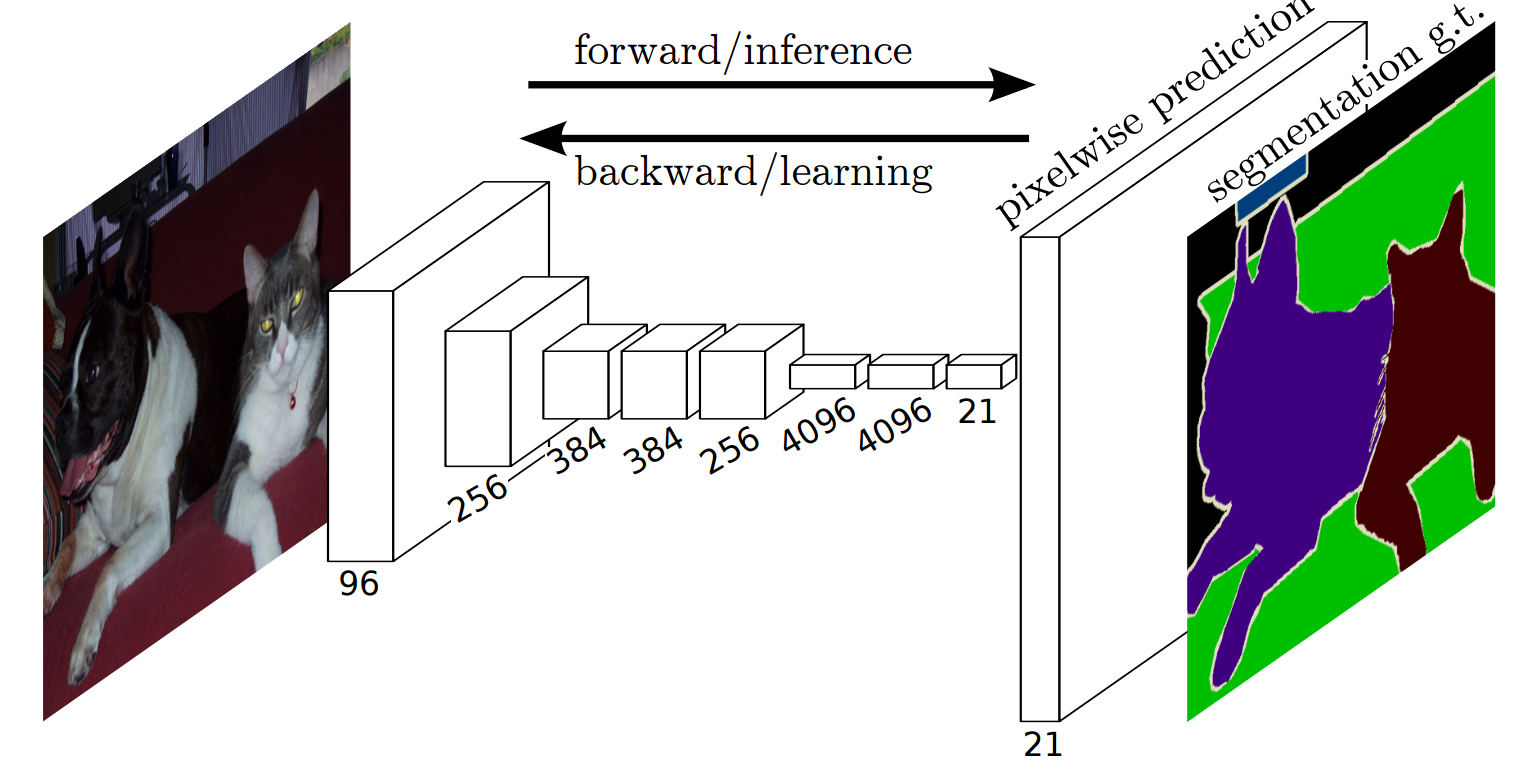
\includegraphics[width = 0.8\textwidth]{images/cat_segmentation.png}
    \caption{Arquitectura de \gls{FCN} obtenida de~\cite{long2015fully}}
    \label{fig:my_label}
\end{figure}
La característica de las \gls{FCN} es que estas poseen 2 partes principalmente.
\begin{itemize}
        \item \textbf{Codificador} Este modulo gradualmente reduce el mapa de características y captura la mayor cantidad de información semántico.
        \item \textbf{Decodificador} : Este modulo gradualmente recupera la información espacial 
    \end{itemize}{}
    
    

\section{Técnicas tradicionales del Análisis forestal}
\subsection{Índices de vegetación }
Según la hoja de apuntes de~\cite{munoz2017apuntes} se pueden clasificar los índices en 2 :
\subsubsection{Índices Basados en la Pendiente}
Los índices basados en la pendiente usan el cociente de la reflectancia de una banda con otra, usualmente el rojo y el \gls{IR} cercano, debido al alto contraste o diferencia en la reflectancia, que presenta la clorofila1en ambas bandas. El término ‘basado en la pendiente’ se refiere a que, al analizar los valores resultantes del índice de vegetación, se compararán esencialmente las pendientes de las líneas que pasan a través del origen y de los pixeles representados en un gráfico, con la reflectancia de una banda en el eje de las X y la reflectancia de la otra en el eje Y.


\begin{figure}[H]
    \centering
    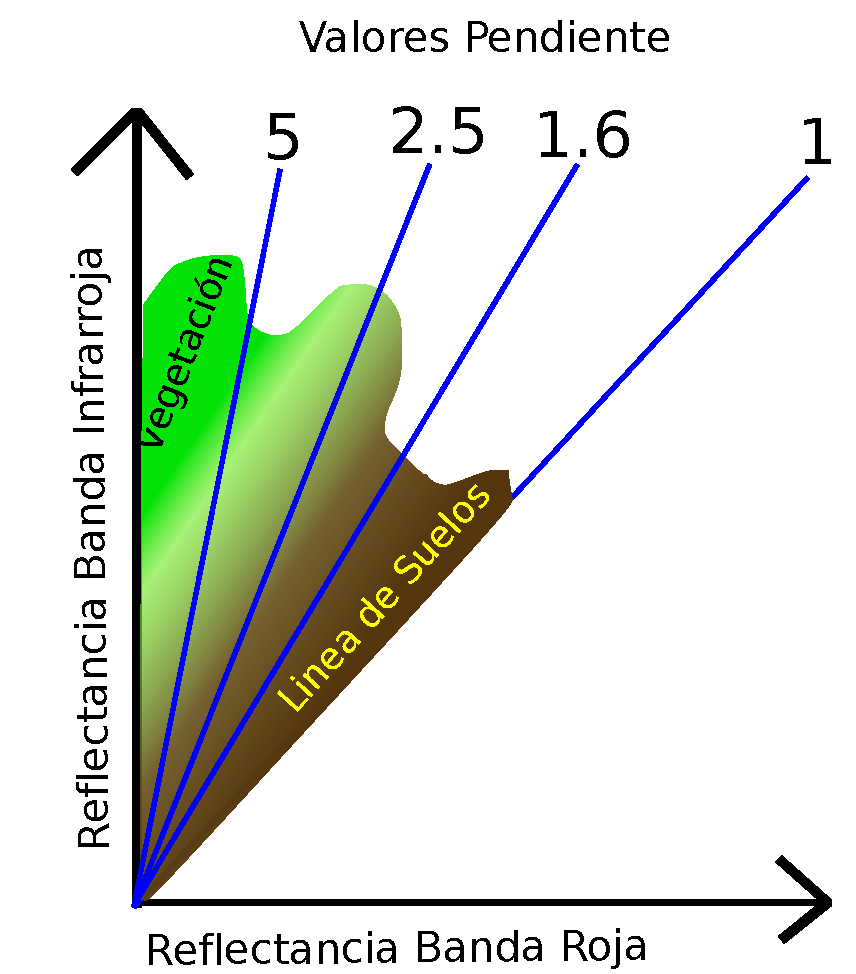
\includegraphics[width=0.4\textwidth]{images/indiceVegetacion.pdf}
    \caption{Gráfica de simulación de índices de vegetación adaptada de~\cite{munoz2017apuntes} }
    \label{fig:indicesBasadosEnLaPendiente}
\end{figure}
\begin{table}[H]
    \centering
    \begin{tabular}{|M{0.10\textwidth}|M{0.35\textwidth}|
   M{0.4\textwidth}|M{0.10\textwidth}| }\rowcolor[HTML]{EFEFEF} 
        \hline Nombre del Índice & Fórmula & Características & Autor y año \\ \hline
  NDVI Diferencia normalizada &$ \scriptsize{NDVI = \frac{NIR-RED}{NIR+RED}} $ & \scriptsize {Minimiza efectos topográficos y produce escala lineal de medición. La escala va de –1 a 1 con el valor cero representando el valor aproximado donde empieza la ausencia de vegetación. Los valores negativos representan superficies sin vegetación.La normalización que realiza, reduce el efecto de la degradación de calibración del sensor y la influencia de los efectos atmosféricos. Gran sencillez matemática.} & Rouse et al.\cite{rouse1973monitoring} \\\hline 
  TVI Transformado& $\scriptsize{NDVI =\sqrt{ \frac{NIR-RED}{NIR+RED}+0.5 }} $ & \scriptsize{El 0,5 evita valores negativos. La raíz cuadrada, intenta corregir los valores que se aproximan a una distribución de Poissone introduce una distribución normal. No elimina todos los valores negativos.} &Rouse et al. \cite{rouse1973monitoring}\\ \hline
 TTVI Transformadade Thiam & $\scriptsize{TTVI = \sqrt{ABS(NDVI + 0.50)}}$ & \scriptsize{El 0.5 corrige la sobre estimación del verde del TVI} &Richardson et al. \cite{richardson1977distinguishing} \\ \hline
 RVI2 Cociente simple & $RVI =\frac{NIR}{RED} $ & \scriptsize{Poco sensible a las condiciones de iluminación, pero mucho a las propiedades ópticas de la tierra.} &Pearson y Miller \cite{pearson1972remote} \\ \hline 
 NRVI3 Cociente simple normalizado&$NRVI = \frac{RVI –1}{RVI + 1}$& \scriptsize{El resultado del NRVI es normalizado. Es similar al NDVI, reduce los efectos de la topografía, la iluminación y los efectos atmosféricos, además de crear una distribución  normal  estadísticamente deseable.}& Perry y Lautenschlager \cite{perry1984functional} \\ \hline 
 NDWI Diferencial de agua normalizado &$NDWI = \frac{NIR -SWIR}{NIR+SWIR} $& \scriptsize{Este índice se utiliza para medir la cantidad de agua que posee la vegetación o el nivel de saturación de humedad que posee el suelo. Los valores que se obtienen oscilan entre -1 y 1, para las zonas con menos humedad}. & Clevers \cite{clevers1988derivation}\\ \hline 
    \end{tabular}
    \caption{Tabla de Índices de Vegetación}
    \label{tab:my_label}
\end{table}

\subsubsection{Índices Basados en la Distancia}
Los valores de reflectancia registrados por el sensor, para cada pixel, constituyen una reflectancia promedio de todos los tipos de coberturas que están dentro desee pixel. Cuando en  zonas áridas y semi áridas la vegetación es dispersa, la reflectancia recibida pertenece tanto a vegetación como suelo. Estos índices, que tratan de separar la información entre la vegetación y el suelo, se basan en el uso de una línea del suelo y las distancias desde ella


\section{Métodos de validación de resultados}
\subsection{Matriz de confusión}
Es una forma gráfica de análisis del desempeño de los algoritmos de clasificación, usualmente se usa con dos clases para etiquetarlos como falsos o verdaderos para definir la predicción y positivos o negativos para definir la clase real de pertenencia, en la \figurename~\ref{figure:confusionmatrix} se puede apreciar una matriz de confusión para un problema de más de dos clases, para este tipo de matrices se considera la diagonal principal en tonalidades rojo como True Positives, por ejemplo para la clase cero se tiene 34 instancias de las cuales 34 han sido clasificadas correctamente, sin embargo para la clase tres se tiene un total de 41 instancias de las cuales sólo 36 fueron clasificadas correctamente y 5 en tonalidades de amarillo fueron clasificadas como otras clases, \begin{figure}[h]
	\centering
	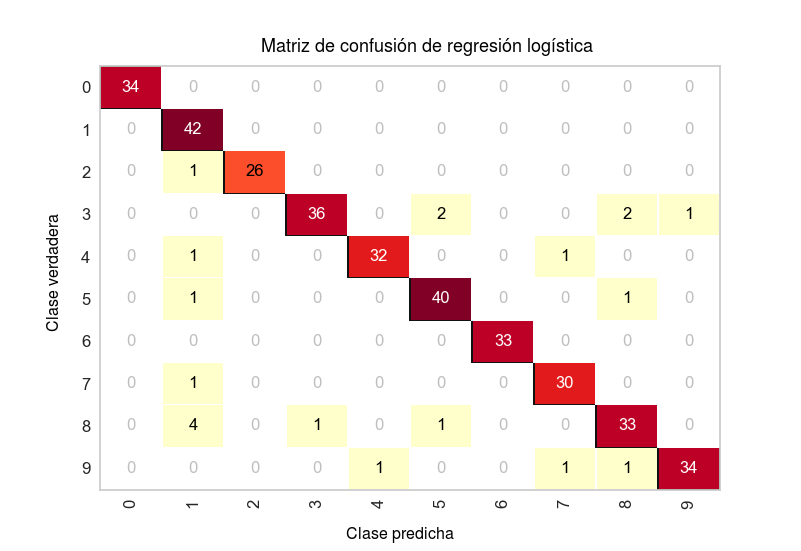
\includegraphics[width=\textwidth]{images/02theory/confusionMatrixEspa.png}
	\caption{Matriz de confusión con más de dos clases, se consideran relevantes los valores de la diagonal principal.}
	\label{figure:confusionmatrix}
\end{figure}


\subsection{Recall y Precisión}
La existencia de muchas instancias negativas es un fenómeno común en muchos sub-campos de la minería de datos y el aprendizaje máquina, por ejemplo muchas de las páginas web son irrelevantes para muchas peticiones. El Accuracy no es una medida de evaluación sensible a la existencia de muchas instancias negativas. Una buena solución es el ignorar los casos que son verdaderos negativos y usar métricas como Recall y Precisión~\cite{Flach2015}
La Precisión esta definida como:
\begin{equation}
 \text{Precision}  = \frac{TP}{TP+FP}
\end{equation}
Donde:
\begin{itemize}
\item \textbf{TP: True Positive} Cantidad de predicciones positivas hechas correctamente.
\item \textbf{FP: False Positive} Cantidad de predicciones positivas hechas incorrectamente.
\end{itemize}

Luego el Recall esta definido como: 

\begin{equation}
 \text{Recall}  = \frac{TP}{TP+FN}
\end{equation}


Donde:
\begin{itemize}
\item \textbf{TP: True Positive} Cantidad de predicciones positivas hechas correctamente.
\item \textbf{FN: False Negative} Cantidad de predicciones negativas hechas incorrectamente.
\end{itemize}
Una forma adicional que mide la relación de desempeño entre el precision y recall es denominada \textbf{F-Measure} definida como:
\begin{equation}
\text{F-Measure}= \frac{2*P*R}{P+R}    
\end{equation}

donde:
P es la precision y R la recall para cierto conjunto de datos.




\section{Segmentación Semántica}
\label{section:metricsevaluation}
\subsection{Métricas para validación de segmentación semántica}
Para que los resultados de segmentación sean buenos se deben usar métricas bien establecidas que permitan validar la utilidad del sistema, en el estado del arte tenemos:
\begin{itemize}
	\item \textbf{Tiempo de ejecución:} Debido al costo computacional de las técnicas utilizadas, es importante conocer el tiempo de entrenamiento de cada una de ellas, es necesario conocer tiempos de cómputo que dependen de hardware específico, brindar tiempos exactos para ciertas configuraciones que permitan tomar decisiones de costos y reproducibilidad de experimentos.
	\item \textbf{Espacios de memoria:} Puede ser un elemento limitante en caso de los modelos que consuman bastante memoria, mantener un reporte de la cantidad de memoria a lo largo de la ejecución del programa se considera necesario para reproducción de experimentos.
	\item \textbf{Accuracy:}  Consiste de métricas que miden la relación del etiquetado por pixel con su objetivo, usualmente variaciones en las precisiones por pixel.
     \begin{itemize}
			\item \textbf{Pixel Accuracy (PA):} Calcula la relación entre el total de pixeles correctamente clasificados y el total de pixeles, definido como: 
			\begin{equation}
			    \text{PA} = \frac{\sum^k_{i=0}p_{ii}}{\sum_{i=0}^{k}\sum_{j=0}^{k} p_{ij}}
			    \end{equation}
			\item \textbf{Mean Pixel Accuraccy (MPA):} Similar al PA descrito arriba con la diferencia de calcular la relación de pixeles correctamente clasificados por clase y luego promediar con el total de clases, se define así:
				\begin{equation}
				\text{MPA} = \frac{1}{k+1}\sum_{i=0}^k\frac{p_{ii}}{\sum_{j=0}^kp_{ij}}
				\end{equation}
			\item \textbf{Mean Intersection over Union (MIoU):} este es el método estándar de evaluación, calcula la relación entre la intersección y la unión de dos conjuntos, en segmentación esto es la relación entre nuestro \textbf{ground truth} y nuestra predicción, se define así: 
			\begin{equation}
			\text{MIoU}= \frac{1}{k+1}\sum_{i=0}^k\frac{p_{ii}}{\sum_{j=0}^k p_{ij}+\sum_{j=0}^{k}p_{ji}-p_{ii}}
			\end{equation}
			\item \textbf{Frecuency Weighted Intersection over Union (FWIoU):} mejora la métrica anterior ponderando la importancia de cada clase con su frecuencia de aparición, definida como:
				\begin{equation}
				    				\text{FWIoU}= \frac{1}{\sum_{i=0}^k \sum_{j=0}^kp_{ij}}\sum_{i=0}^k\frac{\sum_{j=0}^kp_{ij}p_{ii}}{\sum_{j=0}^kp_{ij}+\sum_{j=0}^{k}p_{ji}-p_{ii}}
				    				\end{equation}
		  \end{itemize}
\end{itemize}
Según~\cite{GarciaGarcia2017} \textbf{MIou} es la métrica más usada debido a su simplicidad y representatividad.
\paragraph{Coeficiente de similaridad de Jaccard:} Los índices de similitud son utilizados para el estudio de coexistencia de especies o similitud de sitios de muestreo. Una matriz de coeficientes de similitud, de especies o ubicaciones puede analizarse de dos maneras: por ordenación, es decir, al intentar organizar las ubicaciones o especies dentro de una secuencia teórica continua, o por clasificación, donde se colocan las ubicaciones o especies en grupos discontinuos.
Una manera general como se expresa Jaccard en~\cite{Real1996} es:
\begin{equation}
    J = \frac{C}{A+B-C}
\end{equation}
donde:
\begin{itemize}
    \item A es el número de atributos presentes en un conjunto a.
    \item B es el número de atributos presentes en un conjunto b.
    \item C es el número de atributos presentes en ambos conjuntos a y b.
\end{itemize}
Al coeficiente de Jaccard se le denomina también Intersection over Union, pero para este reporte consideramos Jaccard o \gls{iou}.
\section{Estado del Arte}

En~\cite{Gomez2015} se muestra el desarrollo de metodología para la detección de cambios en series temporales de imágenes Landsat, el autor rellena los datos no útiles (causados por nubes u otros) mediante una interpolación, también el autor plantea una técnica para tratar de predecir el estado actual del bosque basado en la serie temporal, sin embargo demostró que sus resultados de análisis dependen mucho de una data consistente.


El trabajo de~\cite{Vogelmann2012} es un estudio de cambios en varios bosques de Estados Unidos, para esto usaron series temporales de imágenes Landsat, siendo el principal medio de análisis una regresión lineal sobre el Índice Normalizado de Vegetación (NDVI por sus siglas en ingles). El estudio demostró que existen bastantes lugares en los cuales la deforestación va en aumento pero también lugares en los que se esta reforestando.

En~\cite{Saxena2018} menciona que existen distintos algoritmos para la detección de cambios en imágenes satelitales, no obstante el autor menciona que estos algoritmos fueron diseñados para su conjunto de datos, entonces el autor propone usar un conglomerado de algoritmos decidiendo cual usar basado en la distancia de Hausdorff. 


En~\cite{Brooks2017} se muestra las deficiencias de los algoritmos de detección de deforestación causada por factores no tan comunes como son: sequía, enfermedad, actividad de insectos y raleo de cosechas, se propone un algoritmo especializado en detectar los cambios que provienen de dichos factores, su algoritmo esta basado en estadística.


Al igual que el trabajo de~\cite{Saxena2018}, el trabajo~\cite{Healey2018} utiliza la combinación de varios algoritmos, el trabajo se realizó con 8 algoritmos funcionados mediante reglas de fusión basadas en Random Forest, se demuestra la validez de su enfoque probando su algoritmo en imágenes satelitales de varios satélites.

En~\cite{Dutrieux2016} se trata de reconstruir el historial de cambios en base a una serie temporal de imágenes satelitales, para hacer esto utiliza el BFAST (framework Breaks For Additive Season and Trend) que esta especializado en predecir este tipo de actividades, el algoritmo que usaron fue: NDMI (Normalized Difference Moisture Index). En el trabajo se utilizaron todas las imágenes Landsat 7 disponibles de la zona de estudio hasta 5 meses antes de la fecha de publicación. 

% qwerty123
En~\cite{Schroeder2014} muestra como el uso de 2 tipos de imágenes (Landsat y fotografías aéreas) obtienen un resultado con mejor claridad, la primera parte de la metodología incluye una detección de cambios utilizando series temporales Landsat, como consecuencia el uso de la fotografía aérea puede ser más focalizado logrando así reducir costos.

%Se han desarrollado distintos trabajos relacionados a la detección de cambios de suelos Se puede mencionar algunos de los trabajos como son los de :~\cite{Zhu2017}\cite{Khan2016}~\cite{Khan2017}~\cite{Tan2016} que realizan una detección de cambios para un determinado dataset siendo el más común las escenas de LandSat.

%Además existen ciertos trabajos que utilizan redes neuronales para la detección de cambio de suelos como son los de Wang y Zhong\cite{Wang2014}\cite{Zhong2015}.Aunque ambos trabajen con diferente data ambos concuerdan con que trabajar por bloques de imágenes para el entrenamiento es la mejor opción.


%Las resolución subpixel es una herramienta útil para trabajar con imágenes de baja resolución espacial, en~\cite{Wang2014} se mostró que el uso de redes neuronales presenta mejores resultados a los trabajos realizados en resolución subpixel hasta antes de la fecha de publicación del articulo.



En~\cite{Zhong2015} se muestra que el uso de redes neuronales basadas en los sistemas nerviosos de mamíferos pequeños fue utilizado en la detección de cambios en imágenes satelitales, el trabajo combina una red ya estudiada con una característica ya calculada como es el momento normalizado de inercia, el autor indica que el uso combinado del momento de inercia y la red neuronal logra un mejor desempeño que el solo uso de la red neuronal.


En~\cite{SicongLiu2015} se muestra que los pixeles cambiados se pueden subcategorizar para obtener una mejor clasificación, el proceso propuesto por el autor comienza con una técnica basada en la resta de las imágenes, luego se clasifica los pixeles del resultado en 3 grupos, este proceso continua con cada grupo obteniendo, al final un árbol de clasificación en donde cada pixel pertenece a una hoja del árbol.



Otra técnica basada en clusters para la detección de cambios es la propuesta por~\cite{Leichtle2017}, la propuesta esta diseñada para la detección de nuevas edificaciones, el autor realiza un preprocesado basado en propiedades geométricas y análisis de componentes principales para concluir con una clasificación hecha con Kmeans.


Los algoritmos genéticos también pueden ser utilizados para el problema de detección de cambio, en el trabajo de~\cite{Kusetogullari2015} se muestra un método de detección que incluye el algoritmo genético de Particle Swarm Optimization, el autor hace énfasis en su función de fitness y su inicialización de su población para luego comparar su método con otros métodos no supervisados.

En~\cite{Vazquez-Jimenez2017} se trata de realizar la detección de cambios mediante patrones. Se uso como base el método de la transformación de la chi-cuadrada, aunque no se obtuvo resultados sobresalientes, estos fueron lo suficientemente buenos como para que el método se considere viable.

En el trabajo de~\cite{Maggiori2017} se muestra que el problema de etiquetar cada uno de los pixeles puede ser resuelto de distintas maneras. El trabajo muestra que el realizar una red neuronal para cada pixel es ineficiente, es por eso que el autor propone una \gls{FCN} para resolver el problema de una manera más óptima debido al hecho de que la información de pixeles continuos puede ser reutilizada.


\chapter{Base de datos de Imágenes Satelitales}
\label{chap:imagenes}
\section{Descripción de las fuentes de datos}
Las imágenes fueron obtenidas de la pagina de Planet, el proceso para descargar información de la pagina de Planet fue el siguiente:
\begin{enumerate}
    \item Seleccionar el área de interés 
    \begin{figure}[H]
        \centering
        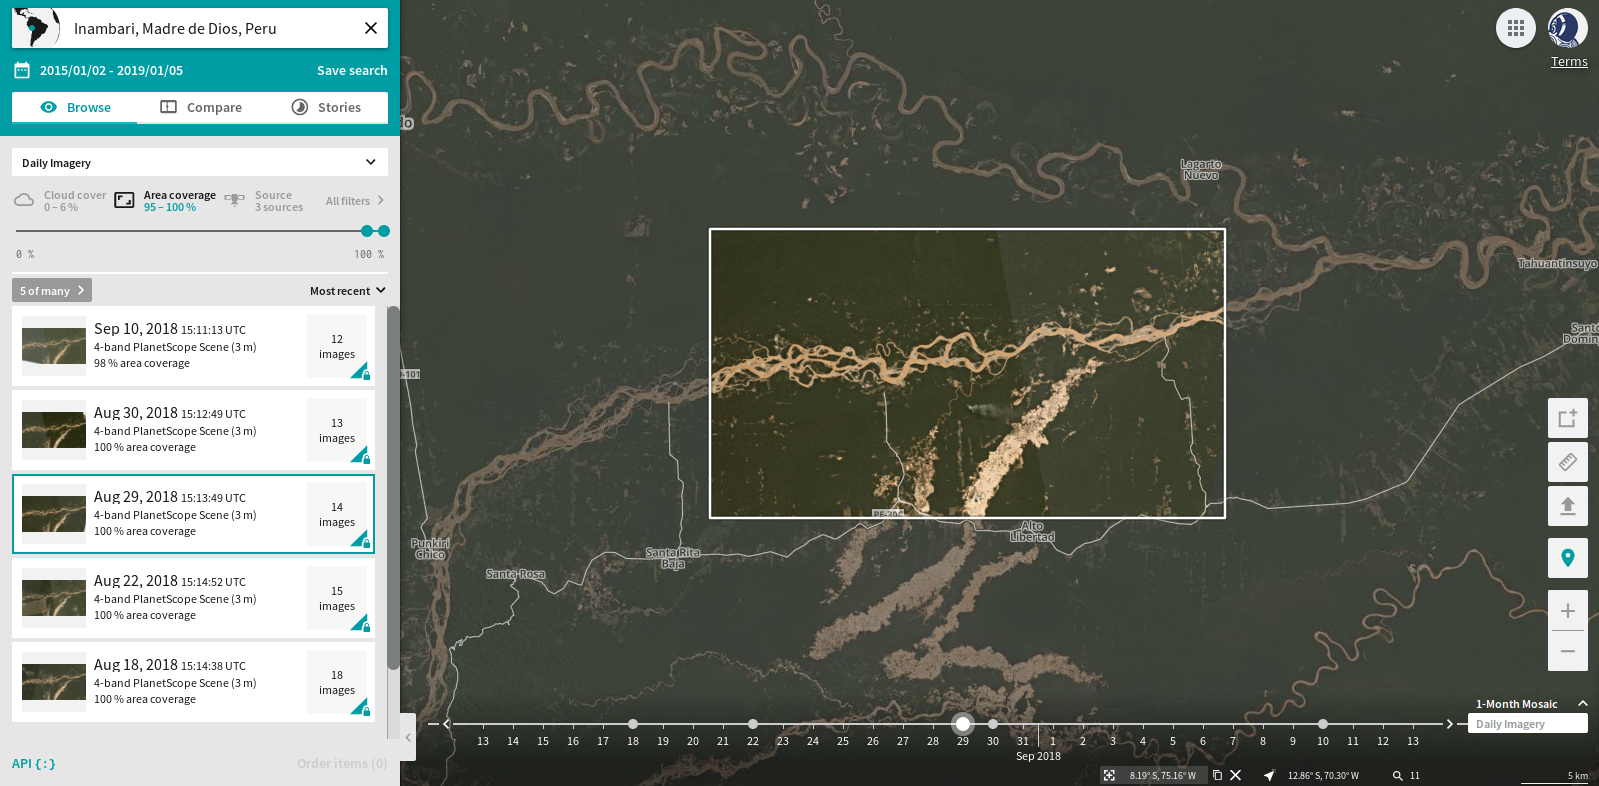
\includegraphics[width = 0.8\textwidth]{images/Imagenes/capturaPlanet.png}
        \caption{Captura de planet que muestra la selección del área de interés}
        \label{fig:my_label}
    \end{figure}
    De lo anterior se tiene que configurar las siguientes preferencias:
    \begin{itemize}
        \item Cobertura de nubes:  0-6\%
        \item Bandas multiespectrales : 3
        \item Fecha de Búsqueda:
    \end{itemize}
    \item  Hacer el pedido  de las imágenes.
    \item Especificar la escena que corresponda.
    
\end{enumerate}

\definecolor{grey1}{gray}{0.6}






\section{Zona de Estudio}
En un estudio provisto por el \gls{MAAP} se definió que existen zonas de deforestación importantes en el sur de la Amazonia peruana (región Madre de Dios). Una de las causas de la deforestación es la minería aurífera entre la carretera Interoceánica y el río Malinowski. La deforestación minera más grave se está extendiendo hacia el este en la zona conocida como La Pampa. Cabe enfatizar que el gobierno peruano acaba de iniciar la “Operación Mercurio 2019” \footnote{https://www.gob.pe/institucion/mininter/noticias/25784-operacion-mercurio-2019-permitira-restituir-el-principio-de-autoridad-en-la-pampa} un operativo multisectorial y integral que tiene como objetivo principal erradicar la minería ilegal y los delitos asociados a ella en la zona de La Pampa, así como impulsar acciones de desarrollo en la región.

El \gls{MAAP}  tambien realizo distintos estudios acerca de la deforestación  causada por la mineria ilegal, determinando que en el año de 2017 se mostro el mayor aumento de deforestacion caisada por mineria aurifera. En dicho estudio se determino que la deforestacion causada pro mineria aurifera fue de unas 9,160 hectareas. A continuacion se detallan algunas de las zonas afectadas 
\subsection{La Pampa}
La \figurename~\ref{fig:LaPampa} muestra la deforestación de 1,685 hectáreas por minería aurífera entre el 2017 (panel izquierdo) y el 2018 (panel derecho), en la zona conocida como La Pampa (región de Madre de Dios). Los círculos rojos indican los principales frentes de deforestación.

\begin{figure}[H]
    \centering
    \includegraphics[width = 1\textwidth]{images/ImagenesMineria/LaPampa.jpg}
        \caption{Slide de los cambios en la zona de La Pampa}

    \label{fig:LaPampa}
\end{figure}
\subsection{ Alto Malinowski}

La \figurename~\ref{fig:AltoMalinowski}  muestra la deforestación de 760 hectáreas por minería aurífera entre el 2017 (panel izquierdo) y el 2018 (panel derecho), en la zona conocida como Alto Malinowski (región de Madre de Dios). Los círculos rojos indican los principales frentes de deforestación.



\begin{figure}[H]
    \centering
    \includegraphics[width = 1\textwidth]{images/ImagenesMineria/AltoMalinowski.jpg}
    \caption{Slide de los cambios en la zona de Alto Malinowski}
    \label{fig:AltoMalinowski}
\end{figure}{}


\subsection{Camanti}




La \figurename~\ref{fig:Camanti}  muestra la deforestación de 335 hectáreas por minería aurífera entre el 2016 (panel izquierdo) y el 2018 (panel derecho), en el distrito de Camanti (región Cusco). Los círculos rojos indican los principales frentes de deforestación. Nótese la creciente proximidad de la minería hacia la Reserva Comunal Amarakaeri\footnote{La Reserva Comunal Amarakaeri (RCAM) tiene una superficie de 402 335,62 hectáreas. Su establecimiento busca contribuir a la protección de las cuencas de los ríos Madre de Dios y Colorado, a fin de asegurar la estabilidad de las tierras y bosques para mantener la calidad y cantidad de agua, el equilibrio ecológico y un ambiente adecuado para el desarrollo de las comunidades nativas Harakmbut}.

\begin{figure}[H]
    \centering
    \includegraphics[width = 1\textwidth]{images/ImagenesMineria/Camanti.jpg}
    \caption{Slide de los cambios en la zona de Camanti}
    \label{fig:Camanti}
\end{figure}{}

\section{Preparación de imágenes}
\subsection{División de Imágenes}
La primera parte consta en dividir las imágenes en zonas más pequeñas, para este modelo se decidió partir cada imagen satelital en imágenes más pequeñas de 256 x 256, esto se realizo mediante la librería de GDAL\footnote{GDAL es una biblioteca traductora para formatos de datos geoespaciales ráster y vectoriales} GDAL\_traslate que esta diseñada para el traslado de información de un archivo a otro, sin embargo dado que este comando solo sirve para separar una sección de la imágenes se recorrerá un bucle definido de la siguiente forma
                 
\begin{lstlisting}[title = Iteración sobre la Imagen]  
    imagen = gdal.Open(direccionImagen)
    band = imagen.GetRasterBand(1)
    xsize = band.XSize
    ysize = band.YSize
    tile_size_x = 256
    tile_size_y = 256
    for i in range(0, xsize, tile_size_x):
        for j in range(0, ysize, tile_size_y):
\end{lstlisting}
Para cada una de las iteraciones definidas en el bucle superior se corto una imagen definida por los siguientes parámetros: 
\begin{itemize}
    \item \textbf{Formato (-of):} El formato de salida de las imágenes es de GeoTiff cada una de las sub-imágenes esta georeferenciada.
    \item \textbf{Ventana (-swir):} Este parámetro determina si se utilizara toda la imagen en el proceso de traslado el parametro requiere la siguiente informacion:
    \begin{itemize}
        \item \textbf{xoff} Posición inicial del eje x.
        \item \textbf{yoff} Posición inicial del eje y.
        \item \textbf{xsize} El tamaño de la imagen en la dimensión x.
        \item \textbf{ysize} El tamaño de la imagen en la dimensión y.
    \end{itemize}
    \item \textbf{Dirección imagen entrada}
    \item \textbf{Dirección imagen salida}
\end{itemize}
Para la preparación de la data de entrenamiento se etiqueto a cada imagen partida con un numero de 5 dígitos.
\subsection{Etiquetado}
Se genero data a partir de la herramienta LabelMe en la cual se definen el area de interes mediante un conjunto de poligonos.
    \begin{figure}[H]
        \centering
        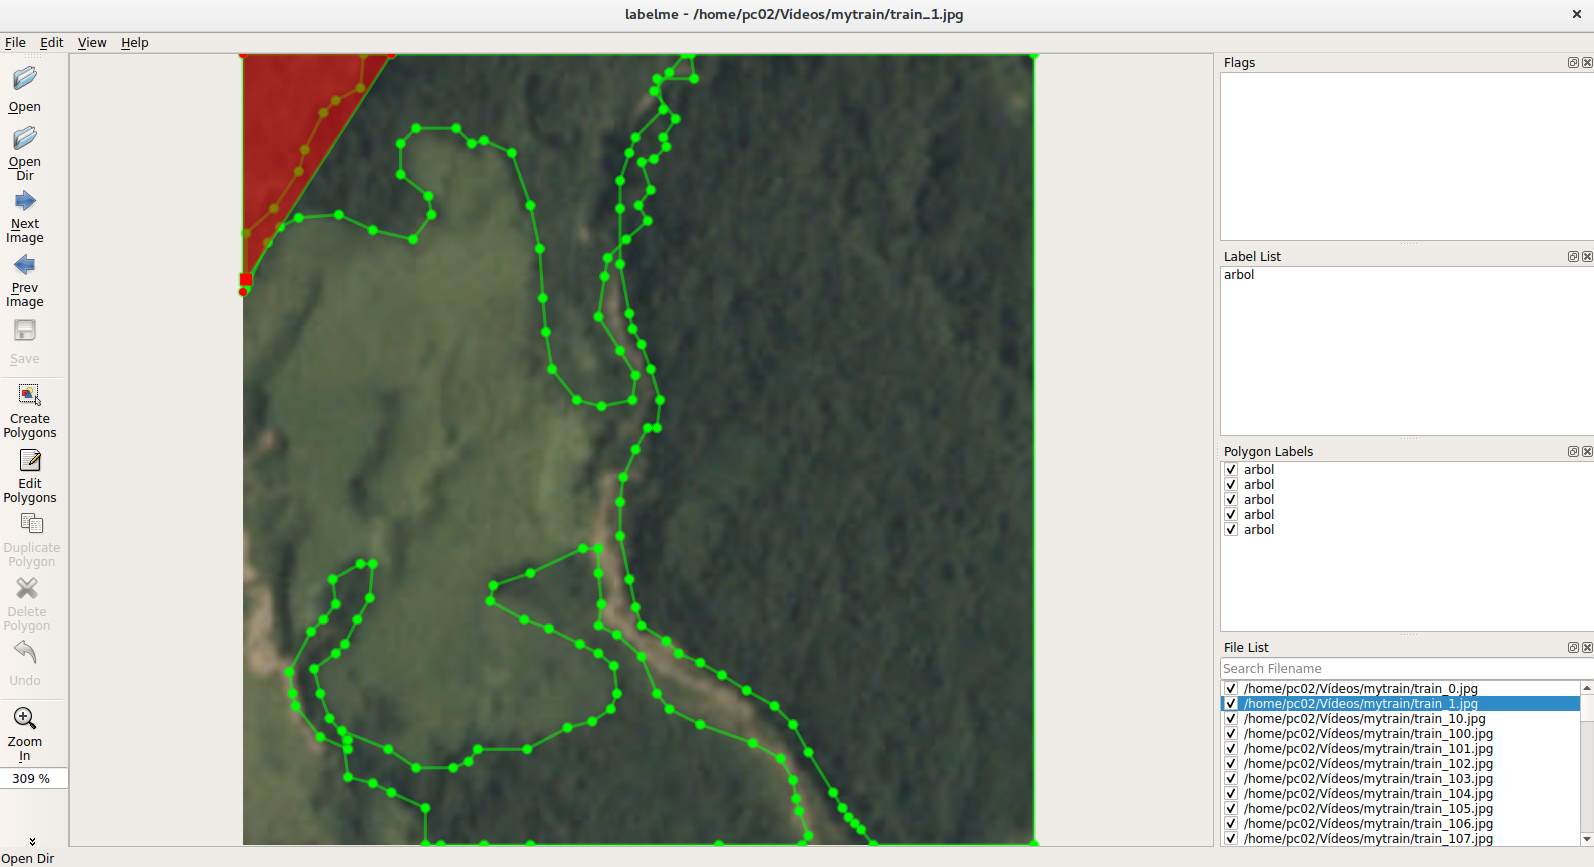
\includegraphics[width=0.8\textwidth]{images/labelme.png}
        \caption{Herramienta LabelMe}
        \label{fig:my_label}
    \end{figure}  
\begin{figure}[H]
	\centering
	\begin{tabular}{cc}
		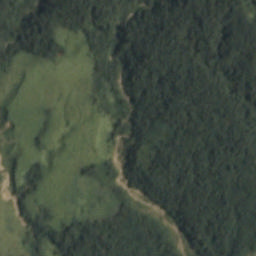
\includegraphics[width=0.3\textwidth]{06changedetection/train_1.jpg} &
		
\includegraphics[width=0.3\textwidth]{06changedetection/label2.png} \\
		a) Imagen original & b) Mascara 				
	\end{tabular}
	\caption{Figuras de muestra utilizadas para el entrenamiento}
	\label{fig:ProblemasVisionComputacional}
\end{figure}
Una vez hecho esto se genero data de entrenamiento adicional mediante las técnicas de aumento de data descritas en la tabla \ref{table:aumentoData} 

\subsection{Descripción Metadata de imágenes}

\begin{table}[H]
    \centering
    \resizebox{13cm}{!}{

    \begin{tabular}{|M{0.2\textwidth}|M{0.9\textwidth}|
   M{0.15\textwidth}|} \hline
            \rowcolor{grey1}             Atributo & Descripción& Tipo \\ \hline


acquired   & El tiempo de adquisición de la imagen en formato RFC 3339.& string \\\hline
anomalous\_pixel& Porcentaje de píxeles anómalos. Píxeles que tienen problemas de calidad en la imagen documentados en la taxonomía de calidad. Esto se representa espacialmente en el UDM(Unusable Data Mask,Mascara que marca los valores no utilizables de la imagen).& number\\\hline

cloud\_cover & Porcentaje de la imagen cubierta por nubes. & number (0 - 1)\\\hline
columns & Numero de columnas en la imagen.& number\\\hline
epsg\_code & Identificador del código del sistema de georeferencia &number\\\hline
ground\_control  & Si la imagen cumple con las especificaciones de precisión posicional, este valor será verdadero. Si la imagen tiene una precisión posicional incierta, este valor será falso. & boolean\\\hline
gsd & El Ground Sampling Distance(Distancia entre los centros de píxeles medidos en el suelo) de la imagen.& number\\\hline
item\_type &El nombre del tipo de elemento que modela el esquema de datos de imágenes compartidas. &string (e.g. “PSScene4Band”)\\\hline
origin\_x & ULX coordinate of the extent of the data. The coordinate
references the top left corner of the top left pixel. &number \\\hline
origin\_y & ULY coordinate of the extent of the data. The coordinate
references the top left corner of the top left pixel. &number\\\hline
pixel\_resolution  & La resolución del pixel de la imagen en metros.& number \\\hline

%Desde aquu abajuyo causa 
provider & Nombre del satélite de procedencia de las imágenes & 
PlanetScope
SkySat
RapidEye
\\ \hline
published & Representa la marca de tiempo RFC 3339 en la que el ítem fue agregado a la API & string\\ \hline
quality\_category	& Métrica para calidad de imagen. Para calificar como calidad “standard”, deben de cumplir con criterios como: altitud del sol $\geq$ 10 grados y ángulo de visión fuera del nadir $<$ 20 grados y píxeles saturados menores al 20\%. Si la imagen no cumple con estos criterios, se califica como calidad de imagen
“test”. & string: "standard" or  "test"\\ \hline
rows& Número de filas en la imagen & number	\\ \hline
satellite\_id& Identificador global único del satélite que adquirió las imágenes subyacentes & string	\\ \hline
strip\_id& Identificador global único de la tira de imagen con la que se recopiló la escena actual & string	\\ \hline
sun\_azimuth & Ángulo desde el norte verdadero hasta donde el vector del sol es proyectado en el plano horizontal en grados & number(0-360)\\ \hline
sun\_elevation & Angulo de elevación del sol en grados & number(0-90)\\ \hline
updated& Representa la marca de tiempo RFC 3339 en la que el ítem fue actualizado en la API & string\\ \hline
usable\_data & Relación de la parte utilizable a inutilizable de las imágenes debido a la cubierta de nubes o al relleno negro. & number(0-1)\\ \hline
view\_angle	& Angulo de visión fuera del nadir a través de la vía espacial utilizado para obtener imágenes, en grados, con + al este y - al oeste.& number(-25 - +25)\\ \hline
    \end{tabular}}
    \caption{Características imágenes planet}
    \label{tab:my_label}
\end{table}

\subsection{Acerca de planet}
Planet Labs es una compañía privada de Satélites de Observación de la Tierra basada en San Francisco, California, EE.UU. La compañía diseña y fabrica satélites de miniatura llamados Doves los cuales una vez listos son lanzados en órbita como carga útil secundaria de otras misiones de lanzamiento satelital. Cada Dove está equipado con un telescopio de alta potencia y una cámara programados para capturar diferente franjas de la Tierra. Cada Dove, satélite de observación de la Tierra, escanea continuamente la Tierra, enviando los datos capturados una vez que pase encima de una estación terrestre de recepción. Juntos, Doves forman una constelación de satélite que entrega una imagen completa de la Tierra todos los días en 3–5m de resolución óptica.

Las imágenes colectadas por los Doves, las cuales pueden ser accedidas en línea cuyas algunas son disponibles bajo una política de acceso libre de datos abiertos, proporciona la información actual pertinente para monitorear el clima, los cambios en el uso del suelo, controlar la deforestación, predecir la cosecha de los cultivos, ordenar la planificación urbana y coordinar la respuesta antes desastre. Con la adquisición de la compañía BlackBridge en julio 2015, Planet Labs tuvieron 87 satélites Doves y 5 satélites RapidEye en órbita. En 2017, Planet lanzó unos 88 satélites Doves adicional y Google le vendió su filial Terra Bella con su constelación de satélite SkySat. La combinación de los satélites Doves forma la mayor constelación nunca puesta en órbita. En septiembre 2018, la compañía había lanzado casi 300 satélites, 150 de los cuales son todavía en actividad.


\subsection{Proceso de Aumento de Data}
Para generar la data de entrenamiento se agrego cierto nivel de ruido con el fin de hacer que el modelo tenga información con ruido.




\begin{table}[H]
\begin{tabular}{|M{0.225\textwidth}|M{0.225\textwidth}|M{0.225\textwidth}|M{0.225\textwidth}|}
\hline
Imagen & Descripción&Imagen & Descripción \\ \hline

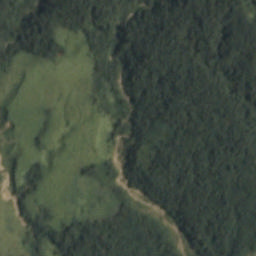
\includegraphics[width=0.225\textwidth]{06changedetection/tranformaciones/original.png}          & \scriptsize{\textbf{Original:} Esta es la imagen original sin ningún procesamiento adicional } &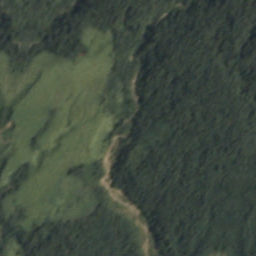
\includegraphics[width=0.225\textwidth]{06changedetection/tranformaciones/shear.png}              & \scriptsize{\textbf{Horizontal Shear:} El proceso consta de transformar la forma de la imagen de un cuadrado a un paralelogramo estirando en un distancia k(0.15\%) la parte inferior a la izquierda  y la parte superior a la derecha, luego de eso se construye la nueva imagen cuadrada obviando las puntas.}         \\ \hline



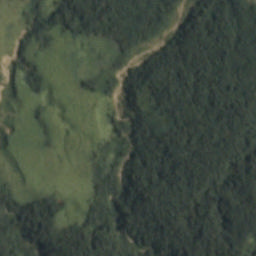
\includegraphics[width=0.225\textwidth]{06changedetection/tranformaciones/arribaAbajo.png}          & \scriptsize{\textbf{Volteo por el eje X :} Se obtiene girando la imagen por el eje x}    &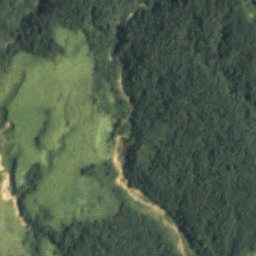
\includegraphics[width=0.225\textwidth]{06changedetection/tranformaciones/gamma.png}     $K$=15         & \scriptsize{\textbf{Filtro Gamma:} Se aplica la siguiente formula a la imagen \smallskip \newline$ I =I^{\frac{1}{1-K}} $ \smallskip \begin{itemize}
\itemsep0em 
 \item I = Imagen Original
 \item K = Tasa de Cambio
\end{itemize}  Luego se escala a 255 niveles }            \\ \hline





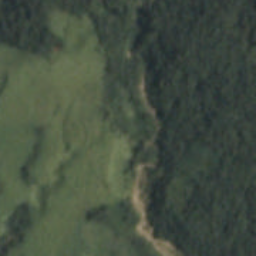
\includegraphics[width=0.225\textwidth]{06changedetection/tranformaciones/rescale.png}             &\scriptsize{\textbf{Cortado Y Escalado:} Se corta una porción de la imagen y esta se escala para que sea del tamaño original  }    &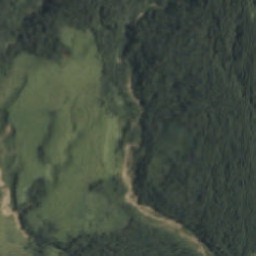
\includegraphics[width=0.225\textwidth]{06changedetection/tranformaciones/elsatica.png}              & \scriptsize{\textbf{Transformación elástica:} Se aplico la técnica para generar data basada en el trabajo de~\cite{simard2003best} que consiste en trazar grillas en la imagen, deformar las grillas y a partir de esto deformar la imagen  }           \\ \hline





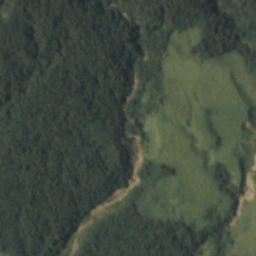
\includegraphics[width=0.225\textwidth]{06changedetection/tranformaciones/izquierdaDerecha.png}              & \scriptsize{\textbf{Volteo por el eje Y:} Se obtiene girando la imagen por el eje Y} &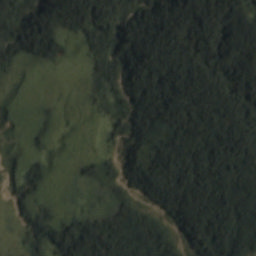
\includegraphics[width=0.225\textwidth]{06changedetection/tranformaciones/escaladoBrillo.png}         $K$=0.2        & \scriptsize{\textbf{Escalado del Brillo :} Se aplicara la siguiente formula a la Imagen \newline$ I =Ix(1-K) $  \smallskip \begin{itemize}
\itemsep0em 
 \item I = Imagen Original
 \item K = Tasa de Cambio
\end{itemize}  }          \\ \hline




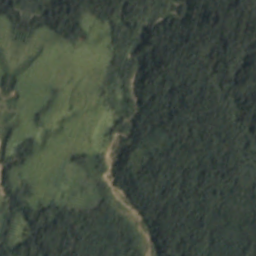
\includegraphics[width=0.225\textwidth]{06changedetection/tranformaciones/rotacion.png} $K$=15     &\scriptsize{\textbf{Rotación :} Se rotara la imagen en un angulo $K$ }    &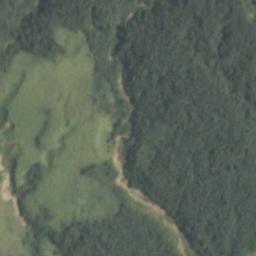
\includegraphics[width=0.225\textwidth]{06changedetection/tranformaciones/moverBrillo.png} $K$=0.15             & \scriptsize{\textbf{Movimiento de Brillo:} Se aplicara la siguiente formula a la Imagen \newline$ I =I+K*255 $  \smallskip \begin{itemize}
\itemsep0em 
 \item I = Imagen Original
 \item K = Tasa de Cambio\end{itemize}  }          \\ \hline
 
 
\end{tabular}

\caption{Tabla de técnicas usadas para aumentar la data inicial}
\label{table:aumentoData} 
\end{table}


\chapter{Desarrollo}
\label{chap:desarrollo}
\section{Marco Teorico}
\label{Sec:Marco Teorico Desarrollo}

\subsection{Arquitectura de La U-Net}
\begin{figure}[H]
	\centering
		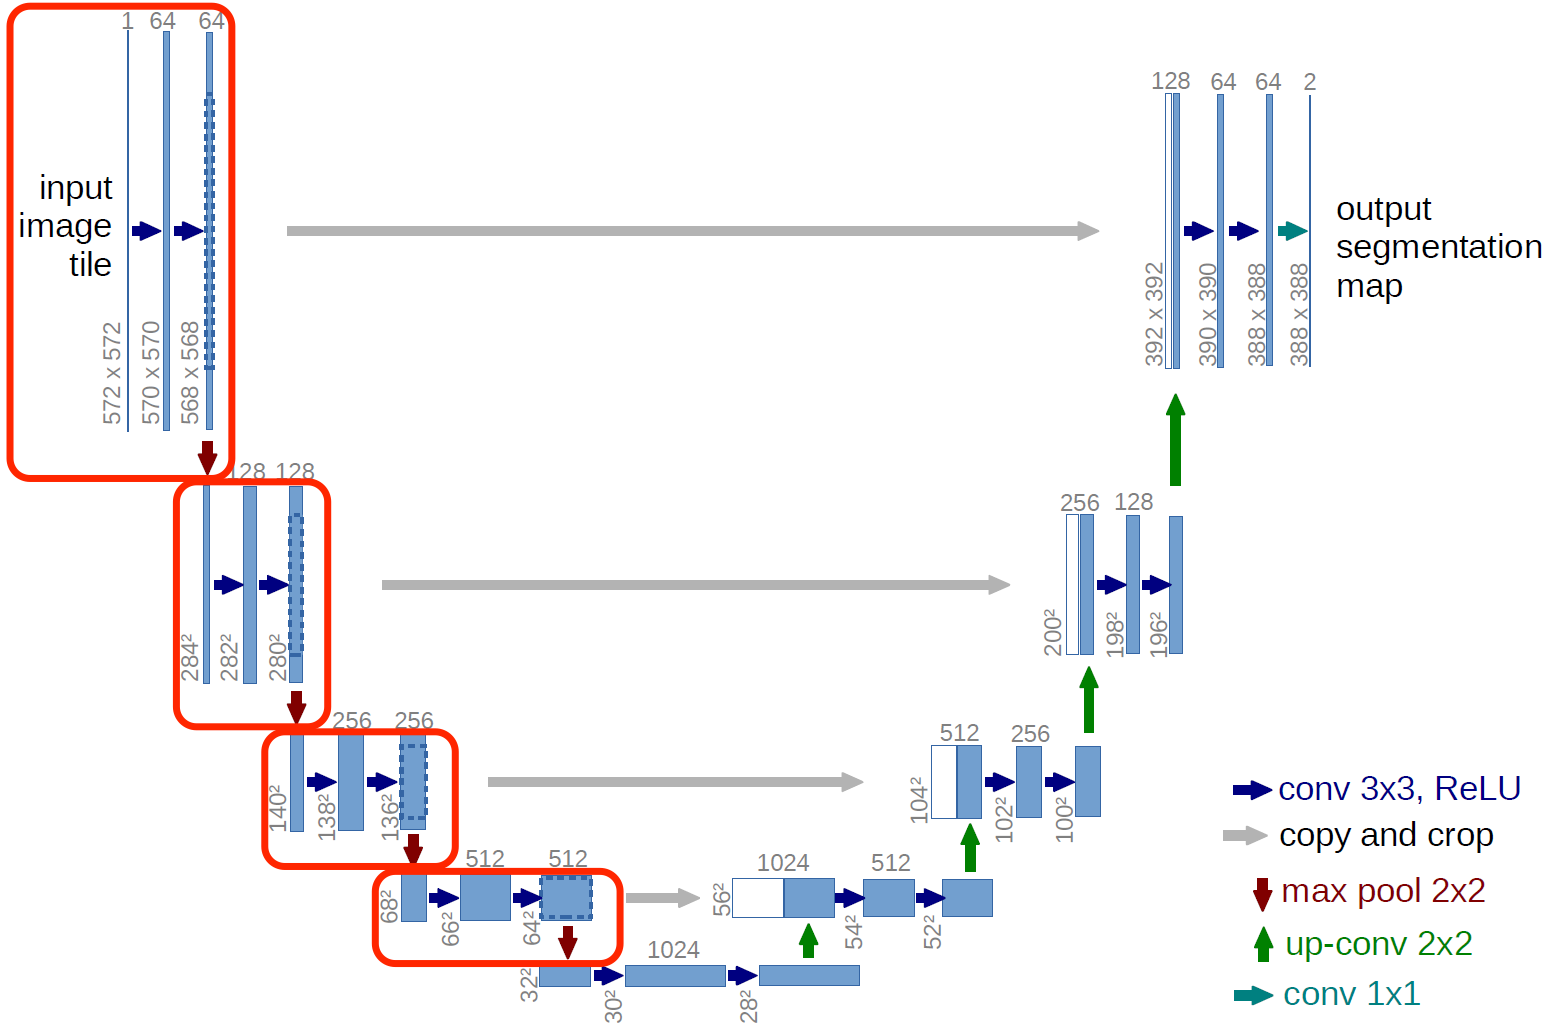
\includegraphics[width=1\textwidth]{06changedetection/unet.png} 
	\caption{Arquitectura original de U-Net}
	\label{fig:ArquitecturaUNET}
\end{figure}

En la \figurename~\ref{fig:ArquitecturaUNET} la arquitectura original de la U-Net~\cite{Ronneberger2015} fue propuesta para imágenes médicas, la U-Net es una red neuronal convolucional realizada para el concurso ``ISBI cell tracking challenge 2015"\footnote{Concurso que consistía en segmentar y rastrear células móviles en secuencias de vídeo.} que consiste en segmentar semánticamente células. La U-Net es caracterizada por que utiliza el copiado de información de las capas de codificación en la sección de decodificación, con esta arquitectura los autores mejoraron los resultados de la segmentación.
La arquitectura comienza con la capa de entrada que es una capa en escala de grises, luego de eso se aplican una serie de convoluciones, la arquitectura tiene 2 partes principales: la de codificación que esta encerrada en rojo y la de decodificación que es el resto. Los tipos de procedimientos usados son:
\begin{itemize}
  \item \textbf{conv 3X3:} Esta es una convolución con filtros de 3 por 3 .
    \item \textbf{copy and crop:} Mediante este proceso se copia la información de las capas codificación en su simétrico de las capas de decodificación.
    \item \textbf{max pool 2x2:} Mediante este proceso se reduce la dimensionalidad de los bloques convolucionales a la mitad para que se pueda procesar mejor.
    \item \textbf{up conv 2x2} Es el proceso para hacer la reconstrucción de la imagen.
\end{itemize}  
La arquitectura propuesta está basada en la U-Net variando las partes del codificador y el decodificador.
\subsection{Bloques residuales}
\label{subsec:residuales}
En el trabajo de \cite{Ruder2016} se presenta el problema de degradación en redes neuronales, este problema se da al aumentar la profundidad la \gls{Accuracy} comienza a bajar. Dicho problema no parece ser natural debido a que si por ejemplo se tiene 2 redes neuronales $a$ y $b$ con $m$ y $n$ capas respectivamente($m$ $>$ $n$), si la red neuronal $a$ utiliza sus $n$ primeras capas de la misma manera que la red $b$, el resto de las capas pueden ser de identidad por la tanto la red neuronal $a$ debería de tener una \gls{Accuracy} por lo menos igual a la red neuronal $b$.  

El problema anterior es resuelto por \cite{Ruder2016} con sus denominados bloques residuales cuya arquitectura esta representado en el siguiente bloque:

\begin{figure}[H]
    \centering
    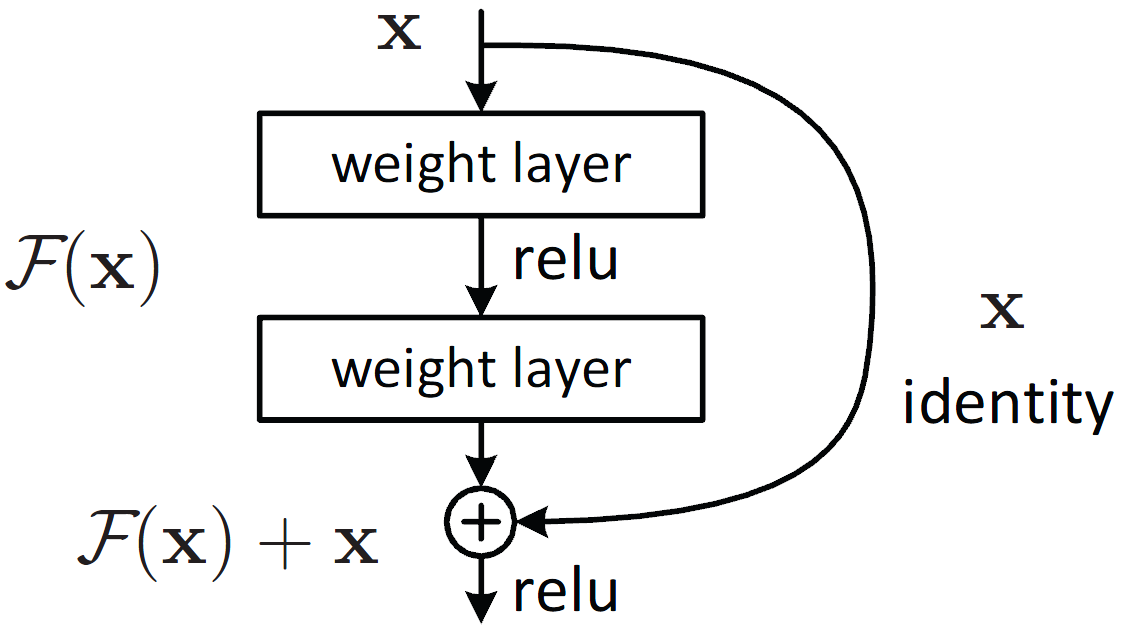
\includegraphics[width =0.7\textwidth]{images/resnet.png}
    \caption{Arquitectura de bloque residual}
    \label{fig:my_label}
\end{figure}


Esta técnica permite a la red neuronal poder transmitir la información de manera más sencilla dado que en caso se necesite la función identidad  los weight layers se asignarían a cero.    
\subsection{Estrategias de partir transformar y mezclar}
Las estrategias de partir transformar y mezclar fueron usados en artículos como \cite{Xie2017, Szegedy2015}, dichas estrategias han demostrado mejorar el rendimiento de las redes neuronal. Por ejemplo \cite{Xie2017} muestra que el uso de estas estrategias lograron una mejora con respecto a sus versiones lineales, esto se aprecia en el siguiente gráfico:
\begin{figure}[H]
    \centering
    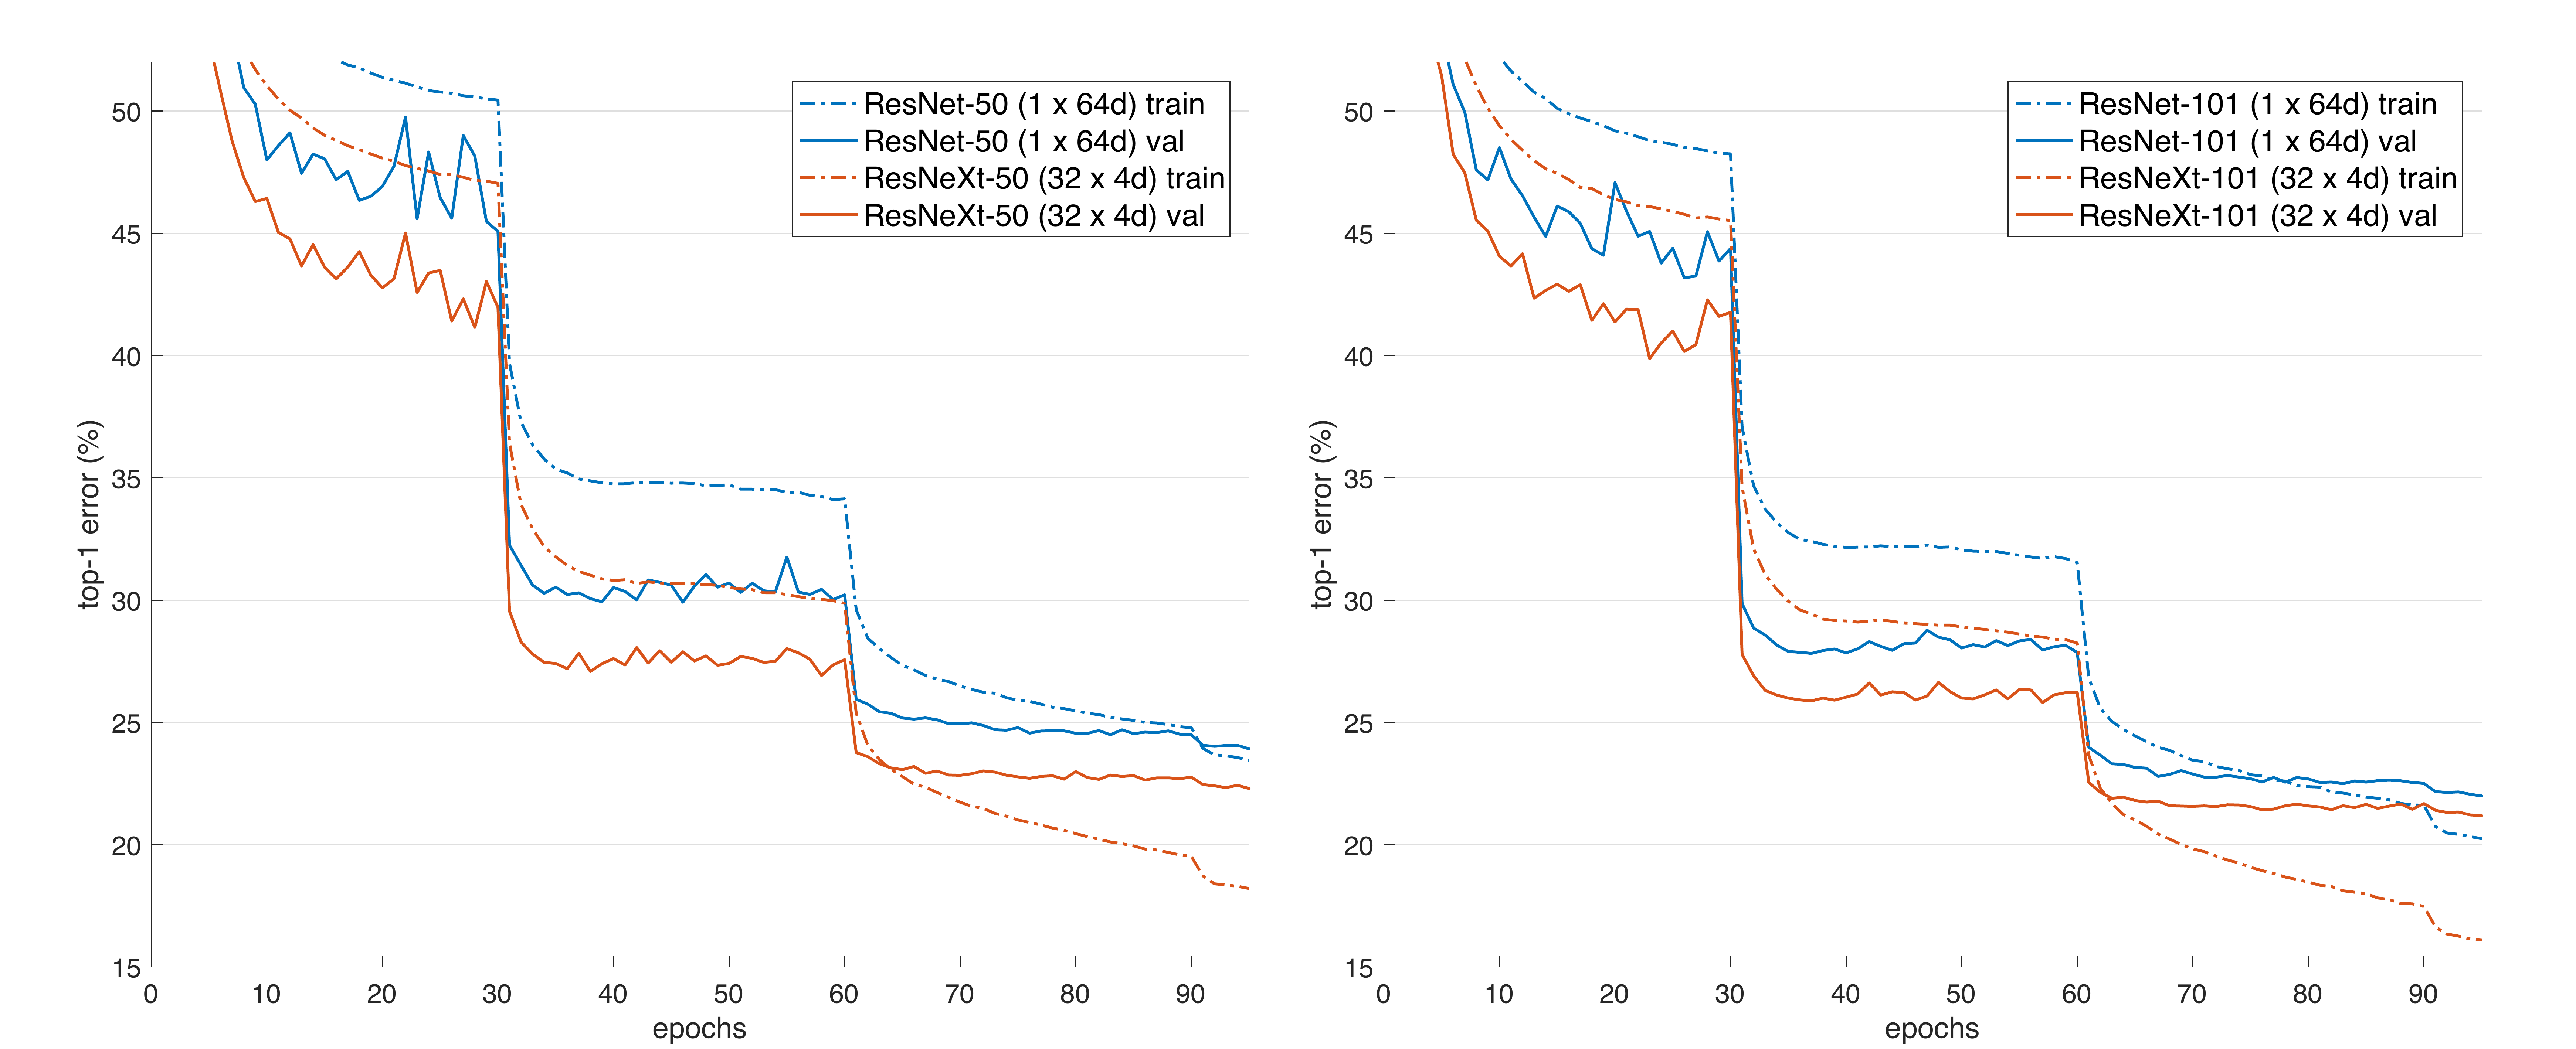
\includegraphics[width=0.9\textwidth]{images/group/resnextMejora.png}
    \caption{Mejora de una Aggregated Transformation propuesta por \cite{Xie2017}}
    \label{fig:mejoraRestnext}
\end{figure}{}
Como se aprecia en la \figurename\ref{fig:mejoraRestnext} el uso de la Aggregated Transformation mejora en alrededor de un 1\% el resultado final, además de acelerar un el proceso de entrenamiento. A continuación se mostraran algunas redes que presentan la estrategia  de partir transformar y mezclar. 
\subsection{Resnext}
\label{subsec:resnext}
La estrategia propuesta por \cite{Xie2017} introduce el concepto de cardinalidad, este concepto para el autor significa la transformación de una convolución en una serie de convoluciones más pequeñas. El siguiente gráfico presenta esa idea: 
\begin{figure}[H]
    \centering
    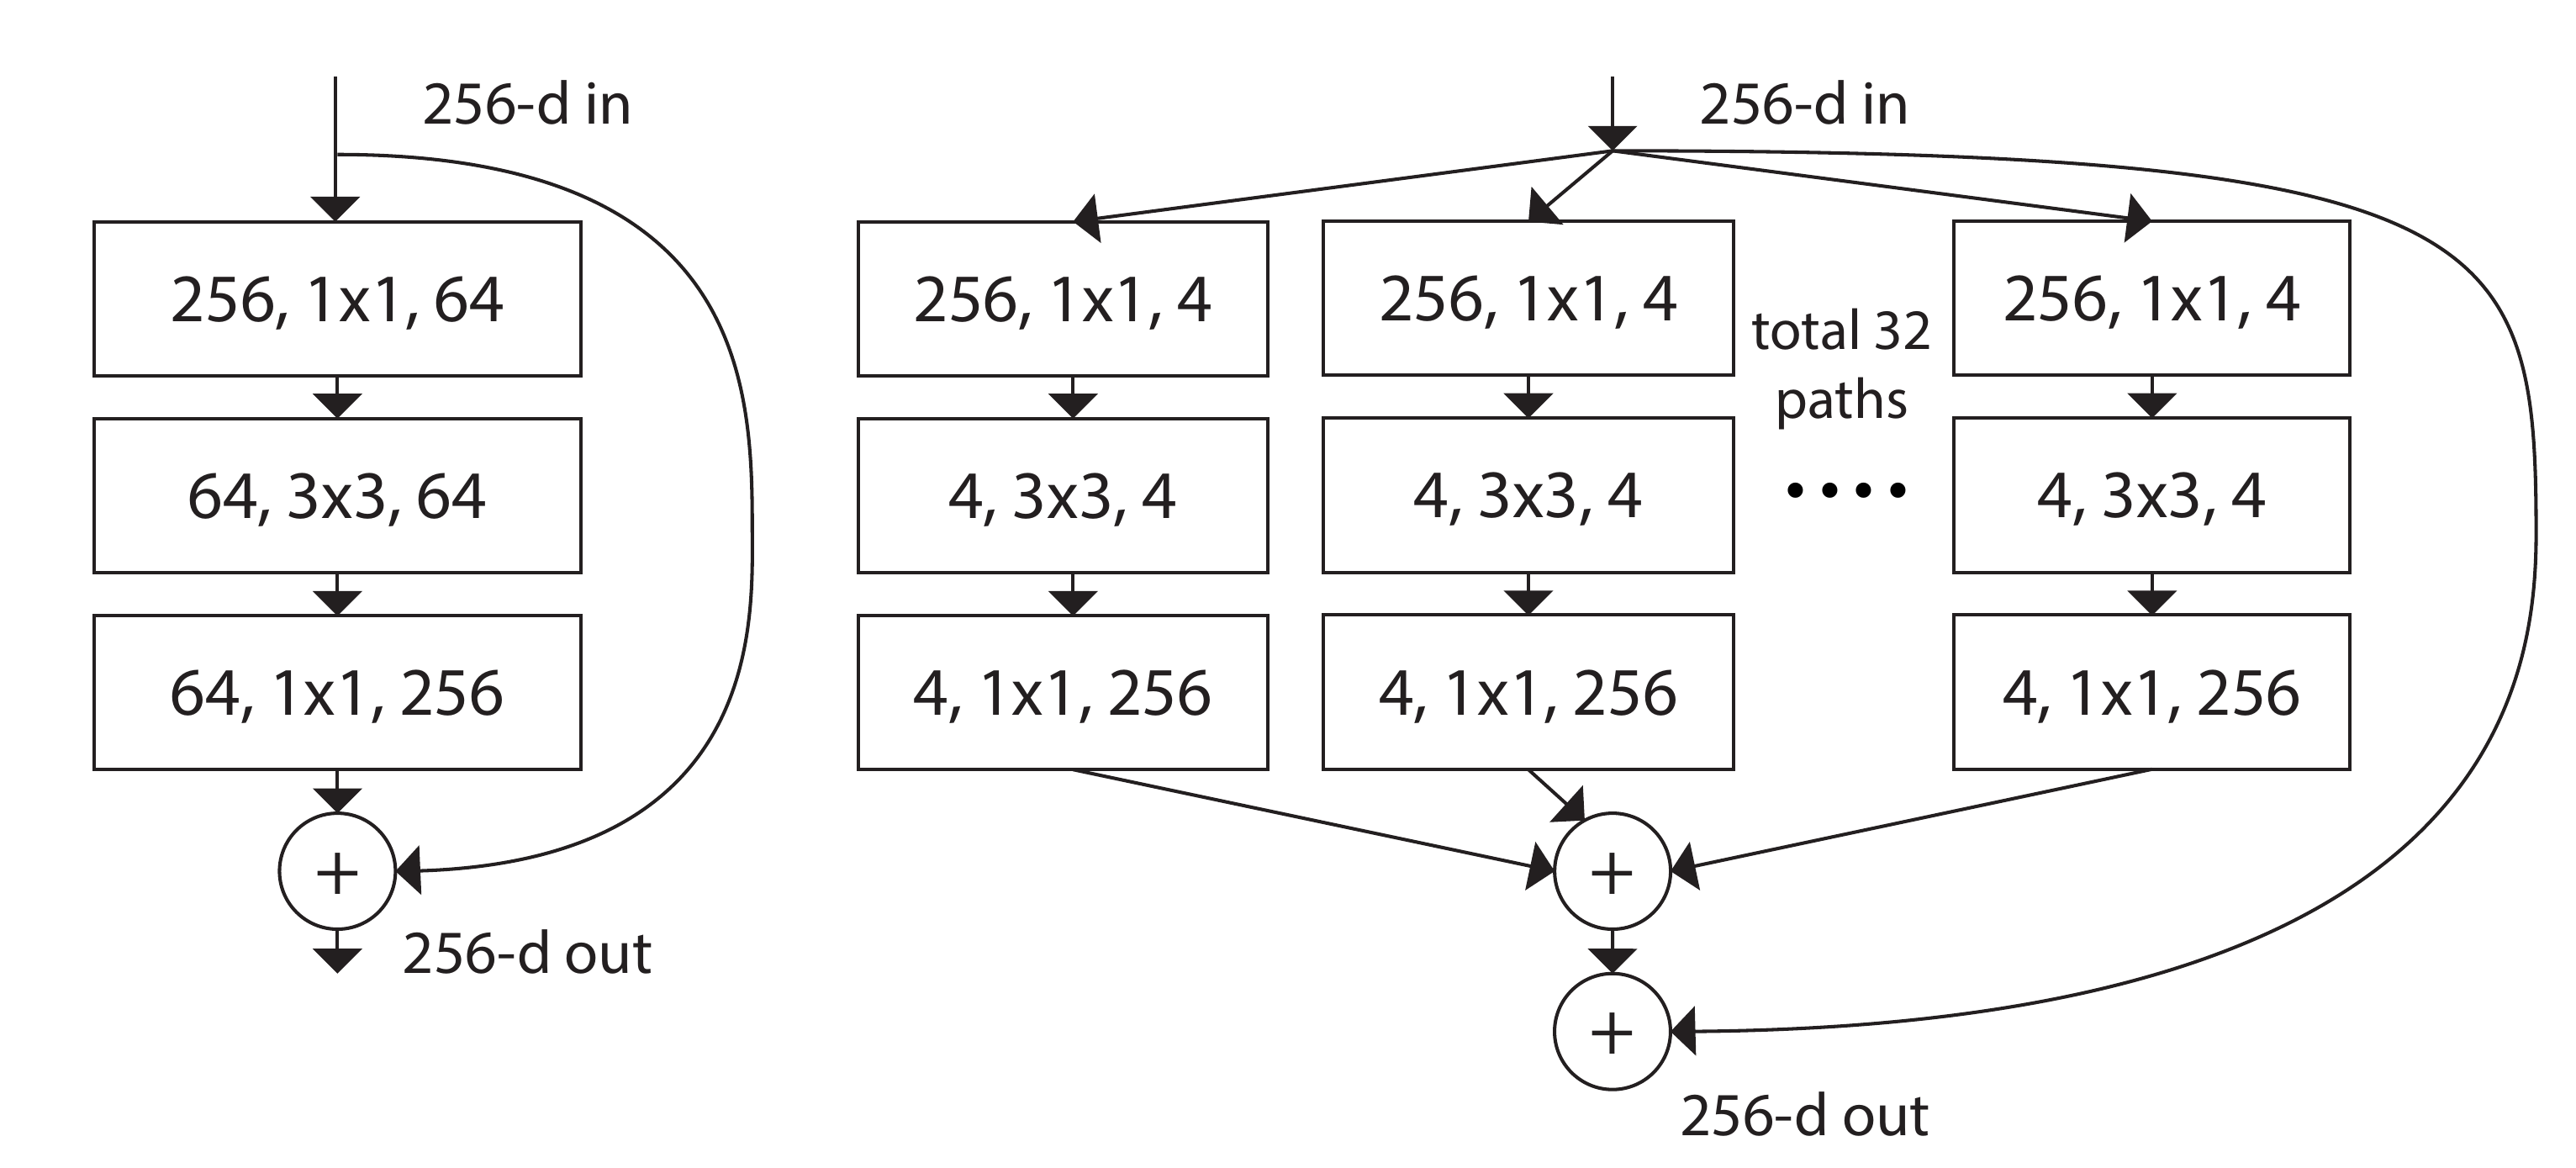
\includegraphics[width= 0.7\textwidth]{images/group/resnext.png}
    \caption{Se muestra el uso de una cardinalidad 32 para el autor propuesto por \cite{Xie2017}}
    \label{fig:resnextBlock}
\end{figure}{}

Como se aprecia en la \figurename \ref{fig:resnextBlock} una series de convoluciones pueden ser transformadas en varias convoluciones más pequeñas, este cambio permite una que estas redes puedan ser operadas en paralelo con más facilidad. 
\subsection{Inception}
La idea de las redes Inception \cite{Szegedy2015} es utilizar múltiples tamaños de filtros para mejorar los resultados, no obstante en este trabajo se demostró que el costo computacional de utilizar múltiples filtros es muy elevada. El autor soluciona este problema utilizando botlenext que es reducir la cantidad de filtros mediante convoluciones 1 x 1, para luego ampliarlas a la cantidad de filtros originales, esto se muestra en la\figurename \ref{fig:inceptionv1} 
\begin{figure}[H]
    \centering
    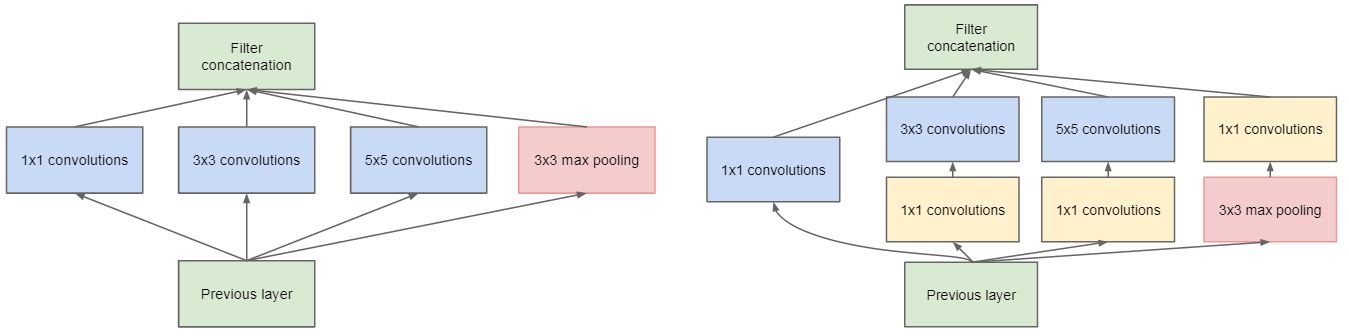
\includegraphics[width= 0.7\textwidth]{images/group/inceptionCortada.png}
    \caption{Arquitectura propuesta en la versión 1 de Google Nets\cite{Szegedy2015}}
    \label{fig:inceptionv1}
\end{figure}{}
Una característica a resaltas de las redes de Google Nets es que cada uno de sus bloques fueron diseñados a comparación de la propuesta de \cite{Xie2017} que se utilizan múltiples bloques iguales.

\subsection{PSP networks}
La Piramid Scene Parsing Networks \cite{zhao2017pyramid} tuvo en consideración el contexto para definir la clasificación de cada pixel, el contexto es obtenido mediante su modulo de conversión piramidal.
\begin{figure}[H]
    \centering
    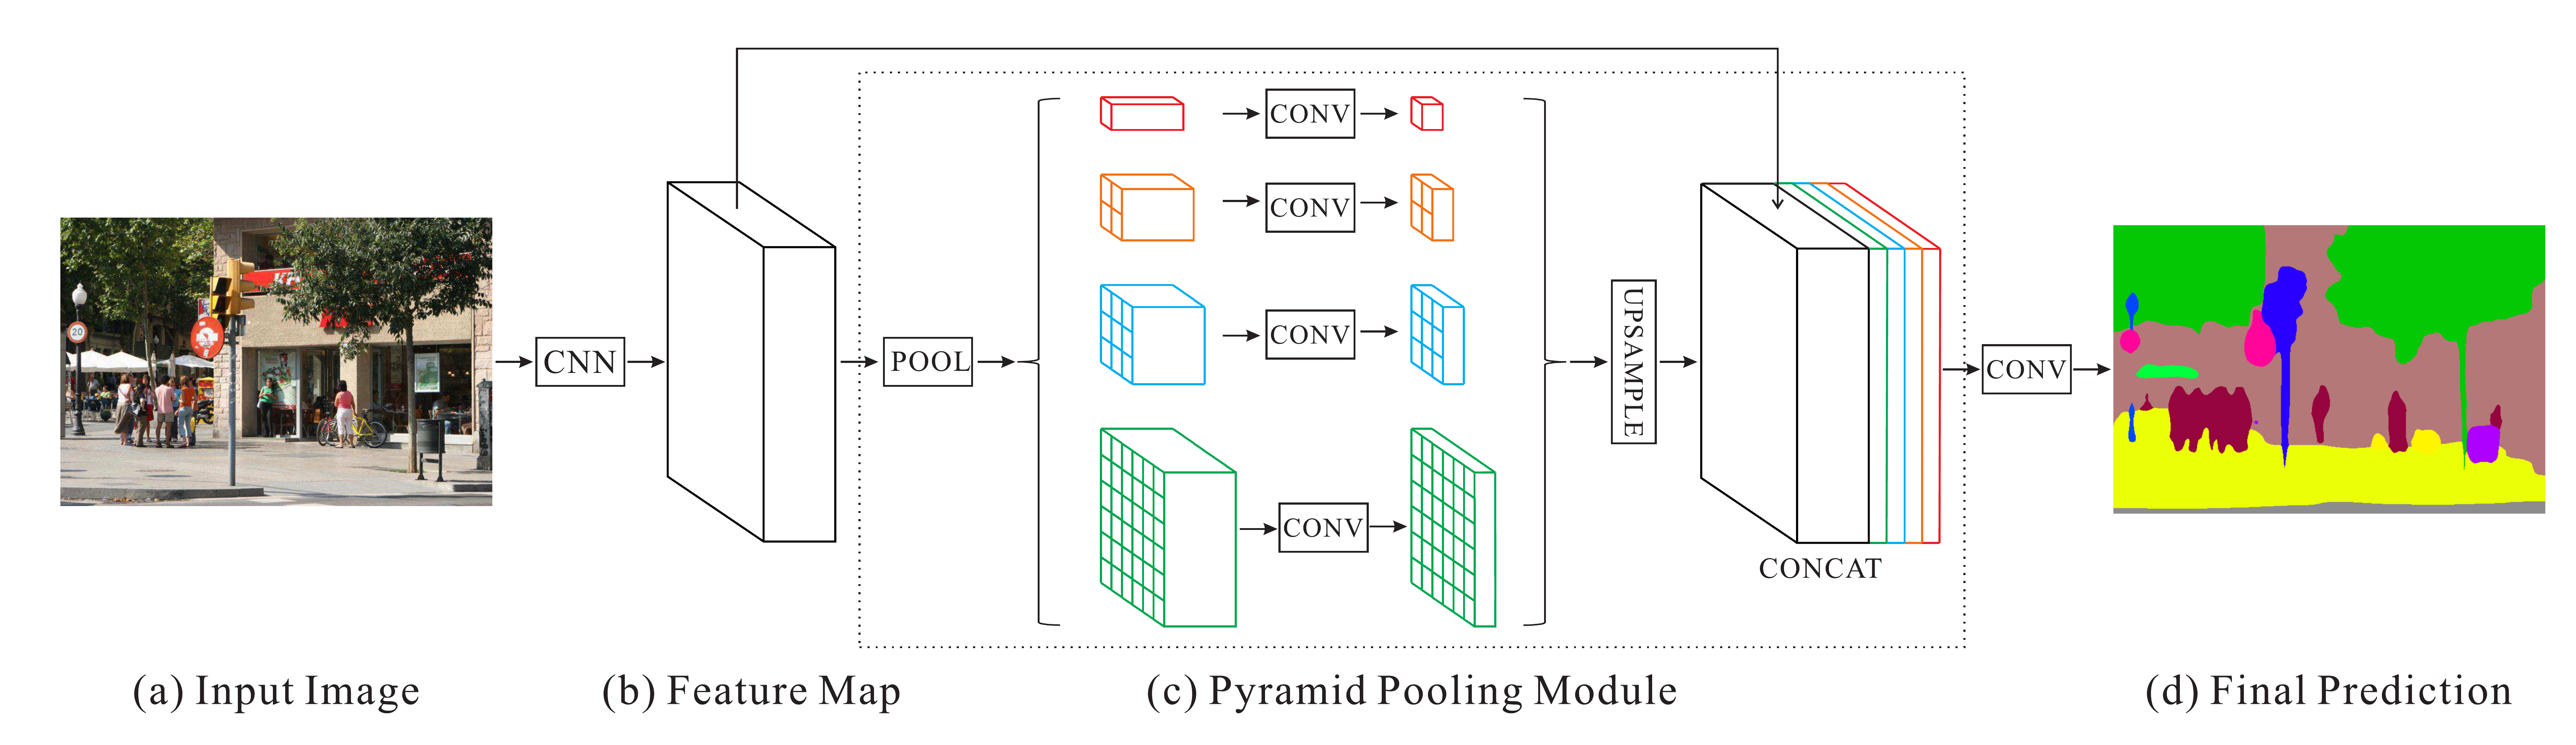
\includegraphics[width = 0.9\textwidth]{images/redes/pspnet.png}
    \caption[Arquitectura PSP]{ Dada una imagen (a), primero se usa una \gls{CNN} para obtener el \gls{Feature Map} para que en la ultimo \gls{Layer}, en (b) el modulo de conversión piramidal es aplicado para obtener distintas representaciones de las subregiones, seguido de un \gls{Upsampling} y concatenación se obtiene el \gls{Feature Map} final, este \gls{Feature Map} porta ambos la información local y la información global contextual. Finalmente el \gls{Feature Map} pasa por unos filtros convolucionales con el fin de obtener un \gls{Layer} por cada clase nesesaria.}
    \label{fig:my_label}
\end{figure}{}
La conversión piramidal se obtiene mediante la aplicación de múltiples tamaños de pooling para que se obtenga la información contextual relacionada a la imagen.

\subsection{Bloque de Squeeze and excitation}
La red convolucional propuesta esta basada en la U-Net, para la parte del codificador se usara una red  basada en el paper de ~\cite{Hu2017} que propone una arquitectura basada en las redes residuales. 
El trabajo propuesto por~\cite{Hu2017} plantea la idea de centrar los esfuerzos de la red en la relación de los canales de un capa convolucional, esto lo hace mediante su técnica de agrupamiento y excitación representada en el siguiente gráfico.
\begin{figure}[H]
	\centering
		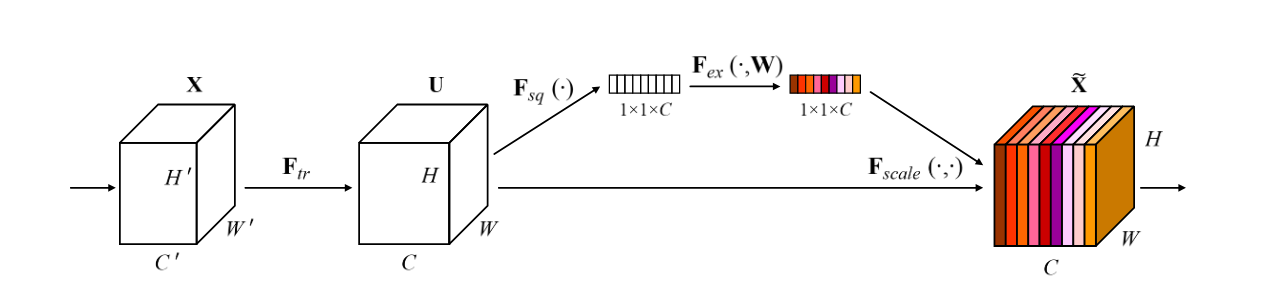
\includegraphics[width=1\textwidth]{06changedetection/SenetBlock.png} 

	\caption[Técnica de agrupamiento y excitación de las SE-Net]{La técnica de agrupamiento y excitación consiste en obtener un valor por cada canal de la capa convolucional luego aplicarle convoluciones al vector resultante para que finalmente los valores obtenidos sean usados como método de  ponderación del bloque convolucional original.}
	\label{fig:Senett}
\end{figure}
En el caso de una red neuronal residual las convoluciones se retransmiten. En el caso de la red neuronal propuesta por~\cite{Hu2017} se procesa un representativo de la capa para poder hacer la convolución correspondiente.

\begin{figure}[H]
	\centering
		\includegraphics[width=0.7\textwidth]{06changedetection/senet_resnet.png} 
	\caption[Comparación ResNet y Se-Resnet]{Imagen comparativa de una red residual normal vs una red de agrupamiento y excitación.}
	\label{fig:Senett}
\end{figure}


Como se menciona en el trabajo de \cite{Liu2015} el contexto para la segmentación semántica juega un papel muy importante, es por eso que autores como: \cite{Liu2015,Yuan2018 ,zhao2017pyramid} desarrollaron distintas propuestas para incluir el contexto en los procesos de las redes neuronales profundas.



\subsection{Decodificador}

La parte del decodificador esta basada en el trabajo de~\cite{Yuan2018}, este trabajo esta basado en el uso de información del contexto para determinar la clase del píxel, su modulo de obtención de contextos puede ser visto como forma de transformar una capa convolucional en otra con mayor información contextual, este proceso fue nombrado en la implementación del autor como bloque de auto Atención. 

%La formula para el bloque es:
%\begin{equation}
%\label{equ:autoContexto}
%    w_{pi}= softmax(\frac{QK^T}{\sqrt{d_K}})V 
%\end{equation}



La arquitectura propuesta usa la idea de \cite{Yuan2018} como operación antes de generalizar el bloque convolucional con una operación de convolución transpuesta que es demostrada en la siguiente imagen:
\begin{figure}[H]
	\centering
		\includegraphics[width=0.7\textwidth]{06changedetection/Transconvolucion.png} 
	
	
	\caption[Procedimiento de una Transconvolución]{Imagen que muestra el procedimiento de una Transconvolución 
}
	\label{fig:Senett}
\end{figure}

\subsection{Función de Perdida }



 La función de perdida usada es la propuesta en el trabajo de \cite{Berman2017} dicha función de perdida  esta basada en el índice de Jaccard descrita previamente en la Sección \ref{section:metricsevaluation} para este trabajo se llamara al índice de Jaccard como \gls{iou}. El autor menciona que su función de perdida fue optimizada para los casos de segmentación semántica.





\subsection{Optimizador}

Se puede considerar a Adam \cite {kingma2014adam}como una combinación de RMSprop y el método de gradiente descendiente con momento. Utiliza las gradientes cuadrados para escalar la velocidad de aprendizaje como RMSprop y aprovecha el momento al usar el promedio móvil del gradiente en lugar del gradiente como SGD con impulso. Adam es un método de tasa de aprendizaje adaptativo, lo que significa que calcula las tasas de aprendizaje individuales para diferentes parámetros. Su nombre se deriva de la estimación del momento adaptativo, y la razón por la que se llama así es porque Adam usa estimaciones del primer y segundo momento del gradiente para adaptar la tasa de aprendizaje para cada peso de la red neuronal.


\section{Descripción de la red neuronal}

\subsection{Bloques utilizados }
\subsubsection{BotleNext}
\begin{figure}[H]
    \centering
    \includegraphics[width=0.9\textwidth]{images/blocks/botlenext.pdf}
    \caption{Modulo Básico del Encoder}
    \label{fig:moduloEncoder}
\end{figure}
Como se aprecia en la figura \ref{fig:moduloEncoder} el modulo básico del encoder es la propuesta en el paper de \cite{Hu2017}, ver la subsección \ref{subsec:residuales} y la subsección \ref{subsec:resnext} 
\begin{enumerate}
    \item  La primera parte es una convolución de 1 x 1 .
    \item  El siguiente modulo es el planteado en la red neuronal ResNext propuesta en el trabajo de \cite{Xie2017}.
    \item  Se pasa a realizar la concatenación de los módulos generados en el paso anterior.
    \item Convolución  de 3 por 3 \label{paso4}
    \item Se comienza con el proceso propuesto por \cite{Hu2017} un adaptative pooling\footnote{El objetivo de este es generar un poling con una salida ya determinada} con resultado final de un solo canal.
    \item Se realiza una convolución 1 x 1.
    \item Se pasa a realizar la multiplicación de cada canal con su respectivo bloque. del bloque obtenido en el paso \ref{paso4} 
\end{enumerate}
\subsubsection{Ocnet Bloque base}
\begin{figure}[H]
    \centering
    \includegraphics[width=0.8\textwidth]{images/blocks/decoder.pdf}
    \caption{Arquitectura OCBase}
    \label{fig:my_label}
\end{figure}
\begin{enumerate}
    \item Se realiza una convolución para reducir la cantidad de \gls{Layer}s del \gls{Feature Map}
    \item Se reduce aun más la cantidad de \gls{Layer}s para obtener 3 grupos denominados Query, key, Value.
    \item Se reducen las dimensiones de la red neuronal con el fin de poder operar el proceso descrito en el paper de \cite{yuan2018ocnet}.
    \item En este caso ademas de reducir las dimensiones se opera realiza la operación de la trasnpuesta.
    \item Multiplicación del Query con el Key
    \item Multiplicacion del Value con el resultado de 5. 
    \item Se reconstruye la dimensionalidad. 
    \item Se duplica la cantidad de Layers mediante convoluciones 3x3.
    \item  Se duplica la cantidad de Layersconvoluciones 3x3.
    \item Se concatena el valor obtenido en 1 con el valor obtenido en 8.
    \item Se reduce la cantidad de \gls{Layer}s convolucionales mediante convoluciones 1x1.
\end{enumerate}{}

\subsubsection{Logit}
\begin{figure}[H]
    \centering
    \includegraphics[width = 0.8\textwidth]{images/blocks/logitv2.pdf}
    \caption{Bloque logit}
    \label{fig:my_label}
\end{figure}{}
\begin{enumerate}
    \item Se realiza un Drop Out.
    \item Convoluciones de 3 x3 para obtener un 16 \gls{Layer}s.
    \item Convoluciones de 1x1 para obtener un \gls{Layer}.
\end{enumerate}{}
\subsection{Arquitectura}
\label{Sec:RedPropuesta}
\begin{figure}[H]
    \centering
    \includegraphics[width=0.8\textwidth]{images/blocks/arquitecturared.pdf}
    \caption{Arquitectura final}
    \label{fig:my_label}
\end{figure}

En esta arquitectura se muestran distintas partes, las descritas en la parte e1,e2,e3,e4,e5  son las partes del encoder, en este proyecto se trabajo con 2 encoders diferentes:
\subsubsection{Encoder Senet-154}
El proceso sera descrito de la siguiente manera 
\begin{enumerate}
    \item \textbf{Entrada-e1}  
       \begin{itemize}
           \item Convolución de 3 x3  con \gls{Stride} 2.
           \item    Normalización por \gls{Batch}es.
            \item    Operación \gls{Relu}.
            \item    convolución d3 3x3 con \gls{Stride}.
           \item    Normalización por \gls{Batch}es.
            \item    Operación \gls{Relu}.
            \item    convolución d3 3x3 con \gls{Stride}.
           \item    Normalización por \gls{Batch}es.
            \item    Operación \gls{Relu}.
       \end{itemize}{}
    \item \textbf{e1-e2:} 1 Bottleneck sin reducción + 3 Bottleneck  sin reducción. 
     \item \textbf{e2-e3:} 1 Botleneck con reducción de Stride 2 + 8 Bottleneck sin reducción. 
     
    \item \textbf{e3-e4:} 1 Botleneck con reducción de Stride 2 + 36 Bottleneck sin reducción.
    \item \textbf{e4-e5:} 1 Botleneck con reducción de Stride 2 + 3 Bottleneck sin reducción.
  %  \item \textbf{e5-c1} 1 Base OCNet module
\end{enumerate}{}
\subsubsection{ Encoder Se-Resnext 51}
El proceso sera descrito de la siguiente manera 
\begin{enumerate}
    \item \textbf{Entrada-e1}  
       \begin{itemize}
        \item Convolución de 3 x3  con \gls{Stride} 2.
           \item    Normalización por \gls{Batch}es.
            \item    Operación \gls{Relu}.
            \item    convolución d3 3x3 con \gls{Stride}.
           \item    Normalización por \gls{Batch}es.
            \item    Operación \gls{Relu}.
            \item    convolución d3 3x3 con \gls{Stride}.
           \item    Normalización por \gls{Batch}es.
            \item    Operación \gls{Relu}.
            
            
            
            
            
       \end{itemize}{}
    \item \textbf{e1-e2:} 1 Bottleneck sin reducción + 3 Bottleneck  sin reducción. 
     \item \textbf{e2-e3:} 1 Botleneck con reducción de Stride 2 + 4 Bottleneck sin reducción. 
     
    \item \textbf{e3-e4:} 1 Botleneck con reducción de Stride 2 + 6 Bottleneck sin reducción.
    \item \textbf{e4-e5:} 1 Botleneck con reducción de Stride 2 + 3 Bottleneck sin reducción.

\end{enumerate}{}
\subsubsection{Decoder}
    \begin{enumerate}
    \item \textbf{e5-c1:} OCNet Bloque Base
    \item \textbf{(c1-e5)-d5:}  Se concatenan los bloques c1 y e5. Luego de esto se  aplica el Bloque Ocnet.
    \item \textbf{(d5-e4)-d4:}  Se concatenan los bloques e4 y d5. Luego de esto se  aplica el Bloque Ocnet.
    \item \textbf{(d4-e3)-d3:}  Se concatenan los bloques e3 y d4. Luego de esto se  aplica el Bloque Ocnet.
    \item \textbf{(d3-e2)-d2:}  Se concatenan los bloques e2 y d3. Luego de esto se  aplica el Bloque Ocnet.
    \item \textbf{(d2-e1)-d1:}  Se concatenan los bloques e1 y d2. Luego de esto se  aplica el Bloque Ocnet.
    


    \end{enumerate}{}


\subsection{Deeplab}
La arquitectura de Deeplab utiliza el concepto de las convoluciones dilatadas mencionada anteriormente en la subsección  \ref{sub:convolucionTranspuesta}.

\begin{figure}[H]
    \centering
    \includegraphics[width = 0.9\textwidth]{images/redes/deeplabv1.pdf}
    \caption{Arquitectura Deeplab obtenida de \cite{Chen2018}}
    \label{fig:deeplabv1}
\end{figure}{}
La imagen a la izquierda muestra la arquitectura propuesta en el trabajo de \cite{zhao2017pyramid} en este modulo se muestra se presenta el Spatial Pyramid Pooling. La parte 2 es una arquitectura parecida a la propuesta en la Unet. La imagen de la derecha muestra la arquitectura propuesta en Deeplabv1 en el cual se utiliza una combinación de las 2 arquitecturas. 

\begin{figure}[H]
    \centering
    \includegraphics[width = 0.9\textwidth]{images/redes/deeplab.pdf}
    \caption{Arquitectura Deeplab obtenida de \cite{Chen2018}}
    \label{fig:my_label}
\end{figure}{}
En la versión 3 de DeepLab se utiliza el concepto de las convoluciones dilatadas, según las hipótesis del autor de DeepLab v3 la utilización de convoluciones dilatadas provee una segmentación semántica más aguda en los bordes, esto debido a que la convolución dilatada tiene mayor cobertura a medida que se aumentan las convoluciones.



%
\section{Estructura del código fuente}

\begin{center}
    \begin{forest}
 dir tree,
  before drawing tree={
    for tree={
      tikz+/.wrap 2 pgfmath args={\node [anchor=west, font=\footnotesize, text=red] at (.east) {L:#1; n:#2};}{level()}{n()}
    }
  }
 [ Proyecto.
[ datasets.
[ \_\_init\_\_.py.]
[ \_\_pycache\_\_.]
[ salt\_identification.py.
]]
[ Final.py.]
[ fold0-submission.csv.]
[ last-model-fold3.pth.]
[ lastModel.pth.]
[ losses.
[ \_\_init\_\_.py.]
[ lovasz\_losses.py.]
[ \_\_pycache\_\_.]
]
[ mitest.py.]
[ models.
[ basenet.py]
[ \_\_init\_\_.py]]]
\end{forest}
   \newpage

    \begin{forest}
 dir tree,
  before drawing tree={
    for tree={
      tikz+/.wrap 2 pgfmath args={\node [anchor=west, font=\footnotesize, text=red] at (.east) {L:#1; n:#2};}{level()}{n()}
    }
  }
 [ Proyecto.
 [models
[ inplace\_abn]
[ oc\_net.py]
[ \_\_pycache\_\_]
[ unet.py]]
[ mytest]
[ mytrain]
[ probarIOU.py]
[ PruebaEnNotebook.ipynb]
[ README.md]
[ requerimientos.txt]
[ runs
[ fold2
[ checkpoints
[ best-accuracy-checkpoint-fold3.pth]
[ best-loss-checkpoint-fold3.pth]
[ best-metric-checkpoint-fold3.pth]
[ last-checkpoint-fold3.pth]]
]]]
\end{forest}
   \newpage
    \begin{forest}
 dir tree,
  before drawing tree={
    for tree={
      tikz+/.wrap 2 pgfmath args={\node [anchor=west, font=\footnotesize, text=red] at (.east) {L:#1; n:#2};}{level()}{n()}
    }
  } [ Proyecto.
  [ runs
[ fold2
[ models
[  best-accuracy-model-fold3.pth]
[ best-loss-model-fold3.pth]
[ best-metric-model-fold3.pth]
[ last-model-fold3.pth]
][ events.out]
][ fold3]
[ fold4]
][ run.sh]
[ test.py]
[ train.py]
[ transforms]
[ utils]
]
\end{forest}
\end{center}
\section{Descripción de los archivos}
En esta sección se describirá brevemente los archivos del sistema
\subsection{Dataset}
\label{sub:database}
Carpeta contenedora del dataLoader\footnote{Herramienta de soporte para cargar los datos en el modelo} el archivo se llama \textbf{saltidentification.py} a continuación se detalla el contenido de cada archivo.
\begin{itemize}        
    \item \textbf{\_\_init.py\_\_:} En este archivo se usara como medio de importación en otras carpetas
    \item \textbf{saltidentification:} Este archivo contiene la información del dataLoader, aquí se definen los modos con los cuales se carga la data, la direcciones se definen en la función \textbf{load\_images\_and\_masks} el cual retorna un diccionario con los siguientes datos 
    \begin{itemize}
        \item \textbf{mask:}Este dato represente el groundTruth del resultado de la segmentación. Su tipo de dato un arreglo tipo float32.
        \item \textbf{image\_id} El identificador de la imagen a procesar.
        \item \textbf{input} Este dato representa la imagen  a trabajar es un arreglo tipo float32.
        
    \end{itemize}
    
    En la función \textbf{load\_images\_and\_masks} es donde se reduce la imagen de 256x256 a 128x128, además es la función donde se define el umbral de la binarización para el entrenamiento.
\end{itemize}
\subsection{Looses }
Carpeta donde se encuentran definidas distintas funciones de perdida utilizadas en el entrenamiento, el principal archivo de esta carpeta es \textbf{lovasz\_losses.py} en donde se implementa la función de perdida definida en \cite{yu2015lov}.
\subsection{Models}
En este carpeta se define los modelos utilizados para la red neuronal.
\begin{itemize}
    \item \textbf{basenet.py} En este red se encuentran definidos todos los encoders que se pueden utilizar :'vgg11', 'vgg13', 'vgg16', 'vgg19','vgg11 \_bn', 'vgg13 \_bn', 'vgg16 \_bn', 'vgg19 \_bn','resnet18', 'resnet34', 'resnet50', 'resnet101', 'resnet152','resnext101 \_32x4d', 'resnext101 \_64x4d','se \_resnet50', 'se \_resnet101', 'se \_resnet152','se \_resnext50 \_32x4d', 'se \_resnext101 \_32x4d', 'senet154','darknet') , sin embargo las redes que comiensan con VGG tiene un bug, no utilizar.
    \item  \textbf{oc \_net.py} Definición del decoder, esta implementación esta basada en el articulo de \cite{yuan2018ocnet}
    \item \textbf{unet.py} En este archivo se ensambla el encoder con su respectivo decoder creando así el modelo de red neuronal ha utilizar para el entrenamiento
\end{itemize}
\subsection{mytrain}
\label{sub:mytrain}
En esta carpeta se encuentran las imágenes utilizadas para el entrenamiento. Las imágenes en esta carpeta presentan el formato de train\_\textbf{id}.jpg o train\_\textbf{id}.tif donde id representa el identificador de la imagen. Se debe tomar en cuenta que no todas las imagenes en esta carpeta seran utilizadas para el entrenamiento, solamente las imágenes cuyo id este en algún archivo que cumpla la siguiente expresión train\_\textbf{id}.json. 
Cada imagen que cumpla la condición definida en el parrafo anterior debera de contar con una carpeta con el siguiente formato train\_\textbf{id}\_json  en dicha carpeta se tendrá el archivo \textbf{label.png} que es la mascara de la segmentación usada como groundTrue. La generación de los archivos de imágenes se puede hacer con el script \textbf{Listarjson.py}.
\subsection{mytest}
\label{sub:mytest}
En esta carpeta se encuentran los archivos para el testeo de la aplicación, igual que la carpeta mytrain se presenta el mismo formato que lo anterior.

\subsection{PruebaEnNotebooks.ipynb}
Archivo que contiene una presentación de validación de resultados,la funcionalidad de este archivo sera mencionado en la subsección \ref{Avances}
\subsection{runs}
Carpeta que contiene los modelos de entrenamiento, esta carpeta tiene varias subcarpetas que corresponden a cada uno de los entrenamientos hechos anteriormente:

\subsection{corre.sh}
\label{sub:corre}
Este archivo contiene el script necesario para ejecutar el entrenamiento. El contenido del scrip es el siguiente :
\begin{lstlisting}

python train.py --vtf --pretrained imagenet --loss-on-center --batch-size 6 
--optim adamw --learning-rate 8    e-4 --lr-scheduler noam --basenet senet154 
--max-epochs 600 --data-fold fold4 --log-dir runs/fold4 
--resume runs/fold4/checkpoints/last-checkpoint-fold4.pth
\end{lstlisting}
De esto si se desea entrenar de nuevo, es nesesario cambiar de directorio de guardado cambiando fold4 por fold5 u otros.


\subsection{tranforms}
Aquí se encuentran los scripts para el aumento de data y la transformación del numpy a tensores de pytorch.
\subsection{utils}
Diferentes scripts que se utilizan en el entrenamiento, los más importantes  son:
\begin{itemize}
    \item \textbf{Metrics} Aquí se definen las métricas para las gráficas de iou u la otra pixel acurracy.
    \item \textbf{adamw} Se define un optimizador.
\end{itemize}
\subsection{train.py}
Este archivo es el que contiene todo el proceso de entrenamiento.

 

\chapter{Pruebas y resultados}
\label{chap:pruebas}
\section{Análisis del entrenamiento de la segmentación semantica}
\subsection{Descripción de los equipos}
Se realizo los entrenamientos con diferentes configuraciones, las especificaciones del equipo utilizado para el entrenamiento son: 
\begin{itemize}
    \item Procesador
    \begin{itemize}
        \item Nombre del Modelo: Intel(R) Core(TM) i7-5930K CPU @ 3.50GHz
        \item Frecuencia maxima:  3700.0000 MHz
     \item Frecuencia minima: 1200.0000 MHz
     \item Arquitectura :  x86\_64
     
    \end{itemize}{}
    \item Tarjeta de video
    \begin{itemize}
        \item Nombre del Modelo: GeForce GTX 1080
        \item Memoria : 8119 MiB
        \item Cantidad : 3
        \item Nucleos Cuda por tarjeta : 2560
        \item Frecuencia base : 1607 
        
    \end{itemize}{}
    \item Memoria RAM : 62 GB 
\end{itemize}{}
Las especificaciones del equipo en CPU fueron :
\begin{itemize}
    \item Memoria : 48 GB
    ·   \item Procesador
    \begin{itemize}
        \item Nombre del Modelo:  Intel(R) Core(TM) i7-7700 CPU @ 3.60GHz
        \item Frecuencia maxima: 4200,0000 MHz
     \item Frecuencia minima: 800,0000 MHz
     \item Arquitectura :  x86\_64
     
    \end{itemize}{}
    

\end{itemize}{}
\subsection{Parámetros de Red}
  \begin{table}[H]
      \centering
            \caption{Parámetros de entrenamiento Redes Neuronales}

      \begin{tabular}{|c|c|} \hline
          Parametro & Cantidad  \\\hline
           Tamaño Batch &   10 \\
           Workers & 3 \\
           Learnign rate  & 0.0008\\
           Optimizador & AdamW \\
           Tamaño Original & 256 \\
           Imágenes Entrenamiento sin Aumento de Data & 1296 \\
           
           Técnicas de aumento de data usados  & 9 \\
           Imágenes de Test & 240 \\\hline
           
           
           
           
           
      \end{tabular}
      \label{tab:my_label}
  \end{table}{}


\subsection{Análisis de funciones de perdida}

\begin{figure}[H]
    \centering
    \includegraphics[width=0.8\textwidth]{images/funciones/comparacionesLos.pdf}
    \caption{Gráfica representando la función de perdida de las Redes Neuronales}
    \label{fig:graficasPerdida}
\end{figure}{}

De la \figurename~\ref{fig:graficasPerdida} se puede concluir lo siguiente :
\begin{itemize}
    \item Cuando se utiliza un encoder más profundo la red neuronal tiende a llegar a un punto de equilibrio más rápido.
    \item Si bien las redes neuronales aun no han llegado a un punto de equilibrio, este se tomo como valido.
\end{itemize}{}


\subsection{Análisis de \gls{Accuracy}}

\begin{figure}[H]
    \centering
    \includegraphics[width=0.8\textwidth]{images/funciones/comparacionesAcc.pdf}
    \caption{Gráfica representando la \gls{Accuracy} de las Redes Neuronales}
    \label{fig:Accuracy}
\end{figure}{}
En la \figurename~\ref{fig:Accuracy} se aprecia el progreso del \gls{Accuracy} a través de iteraciones, de esto se puede deducir lo siguiente 
\begin{itemize}
    \item Una red con un Encoder menos profundo tiende a tener peores resultados.
    \item Una correcta arquitectura de red Neuronal puede lograr obtener mejores resultados con una menor cantidad de capaz.
\end{itemize}

\section{Análisis de evaluación en los datos de test}
\begin{table}[H]
    \centering
        \caption{Tabla de \gls{Accuracy} de cada modelo}

    \begin{tabular}{|c|c|}
    \hline  Red Neuronal  &  \gls{Accuracy}   \\ \hline
         Deeplab ResNext 51   &  0.9883300781		\\
        Unet ResNext 51& 0.9923184482	 \\	
        Unet SeNet154 & 0.9923661665	\\	
   Unet   & 0.9849744524 \\  \hline
    \end{tabular}
    
    \label{tab:Acuracy}
\end{table}{}
\begin{table}[H]
    \centering
    \caption{Tiempo de ejecución de la red neuronal en la computadora de solo CPU}
    \begin{tabular}{|c|c|}
  \hline  Red neuronal & Imágenes por Segundo \\ \hline
        Deeplab ResNext 51&		7.8 \\
Unet	&	8.04 \\
  Unet ResNext 51	&	2.98 \\ 
 Unet SeNet154	&	1.2 \\
 \hline
          
    \end{tabular}
    \label{tab:tablaTiemposCPU}
\end{table}{}
Los resultados del \tablename \ref{tab:tablaTiemposCPU} fueron obtenidos luego de promediar 3 ejecuciones con un tamaño de base de datos de 240 imágenes.
\begin{table}[H]
    \centering
    \caption{Tiempo de ejecución de la red neuronal en la computadora de GPU}
    \begin{tabular}{|c|c|}
  \hline  Red neuronal & Imágenes por Segundo \\ \hline
     Deeplab ResNext 51&	72.26 \\
Unet	&	66.77 \\
  Unet ResNext 51	&	51.26\\ 
 Unet seNet154	&	24.27\\
 \hline
          
    \end{tabular}
    \label{tab:tablaTiemposGPU}
    \end{table}{}

Los resultados del \tablename \ref{tab:tablaTiemposGPU} fue el resultado de promediar los tiempo
\subsection{Resultados Segmentación Semántica}

Como resultado final se puede ver algunas de la imágenes procesadas son:

\begin{table}[H]
\caption{Resultados de Segmentación Semántica }

\begin{tabular}{|M{0.3\textwidth}|M{0.3\textwidth}|M{0.3\textwidth}|}
 \hline Original & Obtenida & Binarizada por umbral \\
 \hline
\medskip  \fbox{\includegraphics[width=0.25\textwidth]{images/datos/train80047.png}}
 &\medskip \fbox{\includegraphics[width=0.25\textwidth]{images/datos/outfileSinBinarizar90001.png}}
  & \medskip\medskip \fbox{\includegraphics[width=0.25\textwidth]{images/datos/outfileBinarizado90001.png}}
  
  \\

 \medskip \fbox{\includegraphics[width=0.25\textwidth]{images/datos/train70047.png}} \medskip 
 &\medskip \fbox{\includegraphics[width=0.25\textwidth]{images/datos/outfileSinBinarizar90000.png}} \medskip 
  &\medskip \fbox{\includegraphics[width=0.25\textwidth]{images/datos/outfileBinarizado90000.png}} \medskip 
\\
\hline

\end{tabular}
\label{table:resultadosSegmentacion}
\end{table}

En los resultados mostrados en le \tablename~\ref{table:resultadosSegmentacion}, la columna sin binarizar muestra la segmentación en escala de grises donde el blanco más intenso en un píxel significa mayor posibilidad a que este pixel sea un árbol.
\begin{table}[H]
\caption{Resultados de Segmentación Semántica }

\begin{tabular}{|M{0.19\textwidth}|M{0.19\textwidth}|M{0.19\textwidth}|M{0.19\textwidth}|M{0.19\textwidth}|}
 \hline Original & Unet Clasica& Unet-ResNext 51 &  Unet-Senet154 & Deeplab \\
 \hline
\medskip  \fbox{\includegraphics[width=0.15\textwidth]{images/imagenesEjemplo/6/img.png}}
 &\medskip \fbox{\includegraphics[width=0.15\textwidth]{images/imagenesEjemplo/6/unet.png}}
  & \medskip\medskip \fbox{\includegraphics[width=0.15\textwidth]{images/imagenesEjemplo/6/unet51.png}}
    & \medskip\medskip \fbox{\includegraphics[width=0.15\textwidth]{images/imagenesEjemplo/6/unet154.png}}
      & \medskip\medskip \fbox{\includegraphics[width=0.15\textwidth]{images/imagenesEjemplo/6/deeplab.png}}
  \\
\medskip  \fbox{\includegraphics[width=0.15\textwidth]{images/imagenesEjemplo/5/img.png}}
 &\medskip \fbox{\includegraphics[width=0.15\textwidth]{images/imagenesEjemplo/5/unet.png}}
  & \medskip\medskip \fbox{\includegraphics[width=0.15\textwidth]{images/imagenesEjemplo/5/unet51.png}}
    & \medskip\medskip \fbox{\includegraphics[width=0.15\textwidth]{images/imagenesEjemplo/5/unet154.png}}
      & \medskip\medskip \fbox{\includegraphics[width=0.15\textwidth]{images/imagenesEjemplo/5/deeplab.png}}
  \\
  \medskip  \fbox{\includegraphics[width=0.15\textwidth]{images/imagenesEjemplo/4/img.png}}
 &\medskip \fbox{\includegraphics[width=0.15\textwidth]{images/imagenesEjemplo/4/unet.png}}
  & \medskip\medskip \fbox{\includegraphics[width=0.15\textwidth]{images/imagenesEjemplo/4/unet51.png}}
    & \medskip\medskip \fbox{\includegraphics[width=0.15\textwidth]{images/imagenesEjemplo/4/unet154.png}}
      & \medskip\medskip \fbox{\includegraphics[width=0.15\textwidth]{images/imagenesEjemplo/4/deeplab.png}}
  \\
  \medskip  \fbox{\includegraphics[width=0.15\textwidth]{images/imagenesEjemplo/3/img.png}}
 &\medskip \fbox{\includegraphics[width=0.15\textwidth]{images/imagenesEjemplo/3/unet.png}}
  & \medskip\medskip \fbox{\includegraphics[width=0.15\textwidth]{images/imagenesEjemplo/3/unet51.png}}
    & \medskip\medskip \fbox{\includegraphics[width=0.15\textwidth]{images/imagenesEjemplo/3/unet154.png}}
      & \medskip\medskip \fbox{\includegraphics[width=0.15\textwidth]{images/imagenesEjemplo/3/deeplab.png}}
  \\
  \medskip  \fbox{\includegraphics[width=0.15\textwidth]{images/imagenesEjemplo/2/img.png}}
 &\medskip \fbox{\includegraphics[width=0.15\textwidth]{images/imagenesEjemplo/2/unet.png}}
  & \medskip\medskip \fbox{\includegraphics[width=0.15\textwidth]{images/imagenesEjemplo/2/unet51.png}}
    & \medskip\medskip \fbox{\includegraphics[width=0.15\textwidth]{images/imagenesEjemplo/2/unet154.png}}
      & \medskip\medskip \fbox{\includegraphics[width=0.15\textwidth]{images/imagenesEjemplo/2/deeplab.png}}
  \\
  \medskip  \fbox{\includegraphics[width=0.15\textwidth]{images/imagenesEjemplo/1/img.png}}
 &\medskip \fbox{\includegraphics[width=0.15\textwidth]{images/imagenesEjemplo/1/unet.png}}
  & \medskip\medskip \fbox{\includegraphics[width=0.15\textwidth]{images/imagenesEjemplo/1/unet51.png}}
    & \medskip\medskip \fbox{\includegraphics[width=0.15\textwidth]{images/imagenesEjemplo/1/unet154.png}}
      & \medskip\medskip \fbox{\includegraphics[width=0.15\textwidth]{images/imagenesEjemplo/1/deeplab.png}}
  \\

\hline

\end{tabular}
\label{table:resultadosSegmentacion}
\end{table}

\subsection{Resultados de Detección de cambios}
Una vez obtenidos las mascaras de segmentación binarias se procederá a realizar las operaciones descritas en el trabajo de \cite{Doshi2018}. Repitiendo la operación XOR del proceso de detección de cambios. El resultado se aprecia en la siguiente figura.
 
 

\begin{figure}[H]
	\centering
	\begin{tabular}{ccc}
\fbox{	\includegraphics[width=0.2\textwidth]{images/datos/outfileBinarizado90001.png}} &
\fbox{		\includegraphics[width=0.2\textwidth]{images/datos/outfileBinarizado90000.png}} &\fbox{\includegraphics[width=0.2\textwidth]{images/datos/cambio.png}}
	\\
		a) Entrada 1  & b) Entrada 2  & c) Resultado XOR \\						
	\end{tabular}
	\caption{Gráficas que muestra el las entradas y salidas de la operación XOR}

	\label{fig:ResultadosXOR}
\end{figure}



%http://sci-hub.tw/10.1016/j.isprsjprs.2013.03.006

\chapter{Conclusiones y trabajos futuros}
\section*{Conclusiones}

\label{chap:conclusiones}

\begin{itemize}
  \item Se logro construir una base de datos de imágenes satelitales obtenidas de Planet y de Kaggle.


 \item La reproducción de distintos trabajos de segmentación semántica usando redes neuronales fue hecho apropiadamente.

 \item Fue posible reconocer cambios en base de diferencia de imágenes.
    \item Como se aprecia en el \tablename~\ref{tab:Acuracy}, si se usa un encoder mas profundo se tiende a obtener mejores resultados. Sin embargo esta mejora es de tan solo el 0.005\% en el caso de la Unet Se-Resnext-51 y Unet SeNet154.
    
    \item El uso de redes neuronales Convolucionales en la detección de cambios es una área de estudio aun en desarrollo, sin embargo el auge de redes neuronales convolucionales a traído como consecuencia la creación de múltiples herramientas para poder desarrollar técnicas basadas en redes neuronales convolucionales de manera más rápida y sencilla.
    \end{itemize}{}



\section{Trabajos futuros}

\bibliographystyle{IEEEtran}
 %\bibliographystyle{apalike}
\bibliography{bibliografia}
\appendix
\chapter{Software implementado para el sistema}

\section{Estructura del código fuente}

\begin{center}
    \begin{forest}
 dir tree,
  before drawing tree={
    for tree={
      tikz+/.wrap 2 pgfmath args={\node [anchor=west, font=\footnotesize, text=red] at (.east) {L:#1; n:#2};}{level()}{n()}
    }
  }
 [ Proyecto.
[ datasets.
[ \_\_init\_\_.py.]
[ \_\_pycache\_\_.]
[ salt\_identification.py.
]]
[ Final.py.]
[ fold0-submission.csv.]
[ last-model-fold3.pth.]
[ lastModel.pth.]
[ losses.
[ \_\_init\_\_.py.]
[ lovasz\_losses.py.]
[ \_\_pycache\_\_.]
]
[ mitest.py.]
[ models.
[ basenet.py]
[ \_\_init\_\_.py]]]
\end{forest}
   \newpage

    \begin{forest}
 dir tree,
  before drawing tree={
    for tree={
      tikz+/.wrap 2 pgfmath args={\node [anchor=west, font=\footnotesize, text=red] at (.east) {L:#1; n:#2};}{level()}{n()}
    }
  }
 [ Proyecto.
 [models
[ inplace\_abn]
[ oc\_net.py]
[ \_\_pycache\_\_]
[ unet.py]]
[ mytest]
[ mytrain]
[ probarIOU.py]
[ PruebaEnNotebook.ipynb]
[ README.md]
[ requerimientos.txt]
[ runs
[ fold2
[ checkpoints
[ best-accuracy-checkpoint-fold3.pth]
[ best-loss-checkpoint-fold3.pth]
[ best-metric-checkpoint-fold3.pth]
[ last-checkpoint-fold3.pth]]
]]]
\end{forest}
   \newpage
    \begin{forest}
 dir tree,
  before drawing tree={
    for tree={
      tikz+/.wrap 2 pgfmath args={\node [anchor=west, font=\footnotesize, text=red] at (.east) {L:#1; n:#2};}{level()}{n()}
    }
  } [ Proyecto.
  [ runs
[ fold2
[ models
[  best-accuracy-model-fold3.pth]
[ best-loss-model-fold3.pth]
[ best-metric-model-fold3.pth]
[ last-model-fold3.pth]
][ events.out]
][ fold3]
[ fold4]
][ run.sh]
[ test.py]
[ train.py]
[ transforms]
[ utils]
]
\end{forest}
\end{center}
\section{Descripción de los archivos}
En esta sección se describirá brevemente los archivos del sistema
\subsection{Dataset}
\label{sub:database}
Carpeta contenedora del dataLoader\footnote{Herramienta de soporte para cargar los datos en el modelo} el archivo se llama \textbf{saltidentification.py} a continuación se detalla el contenido de cada archivo.
\begin{itemize}        
    \item \textbf{\_\_init.py\_\_:} En este archivo se usara como medio de importación en otras carpetas
    \item \textbf{saltidentification:} Este archivo contiene la información del dataLoader, aquí se definen los modos con los cuales se carga la data, la direcciones se definen en la función \textbf{load\_images\_and\_masks} el cual retorna un diccionario con los siguientes datos 
    \begin{itemize}
        \item \textbf{mask:}Este dato represente el groundTruth del resultado de la segmentación. Su tipo de dato un arreglo tipo float32.
        \item \textbf{image\_id} El identificador de la imagen a procesar.
        \item \textbf{input} Este dato representa la imagen  a trabajar es un arreglo tipo float32.
        
    \end{itemize}
    
    En la función \textbf{load\_images\_and\_masks} es donde se reduce la imagen de 256x256 a 128x128, además es la función donde se define el umbral de la binarización para el entrenamiento.
\end{itemize}
\subsection{Looses }
Carpeta donde se encuentran definidas distintas funciones de perdida utilizadas en el entrenamiento, el principal archivo de esta carpeta es \textbf{lovasz\_losses.py} en donde se implementa la función de perdida definida en \cite{yu2015lov}.
\subsection{Models}
En este carpeta se define los modelos utilizados para la red neuronal.
\begin{itemize}
    \item \textbf{basenet.py} En este red se encuentran definidos todos los encoders que se pueden utilizar :'vgg11', 'vgg13', 'vgg16', 'vgg19','vgg11 \_bn', 'vgg13 \_bn', 'vgg16 \_bn', 'vgg19 \_bn','resnet18', 'resnet34', 'resnet50', 'resnet101', 'resnet152','resnext101 \_32x4d', 'resnext101 \_64x4d','se \_resnet50', 'se \_resnet101', 'se \_resnet152','se \_resnext50 \_32x4d', 'se \_resnext101 \_32x4d', 'senet154','darknet') , sin embargo las redes que comiensan con VGG tiene un bug, no utilizar.
    \item  \textbf{oc \_net.py} Definición del decoder, esta implementación esta basada en el articulo de \cite{yuan2018ocnet}
    \item \textbf{unet.py} En este archivo se ensambla el encoder con su respectivo decoder creando así el modelo de red neuronal ha utilizar para el entrenamiento
\end{itemize}
\subsection{mytrain}
\label{sub:mytrain}
En esta carpeta se encuentran las imágenes utilizadas para el entrenamiento. Las imágenes en esta carpeta presentan el formato de train\_\textbf{id}.jpg o train\_\textbf{id}.tif donde id representa el identificador de la imagen. Se debe tomar en cuenta que no todas las imagenes en esta carpeta seran utilizadas para el entrenamiento, solamente las imágenes cuyo id este en algún archivo que cumpla la siguiente expresión train\_\textbf{id}.json. 
Cada imagen que cumpla la condición definida en el parrafo anterior debera de contar con una carpeta con el siguiente formato train\_\textbf{id}\_json  en dicha carpeta se tendrá el archivo \textbf{label.png} que es la mascara de la segmentación usada como groundTrue. La generación de los archivos de imágenes se puede hacer con el script \textbf{Listarjson.py}.
\subsection{mytest}
\label{sub:mytest}
En esta carpeta se encuentran los archivos para el testeo de la aplicación, igual que la carpeta mytrain se presenta el mismo formato que lo anterior.

\subsection{PruebaEnNotebooks.ipynb}
Archivo que contiene una presentación de validación de resultados,la funcionalidad de este archivo sera mencionado en la subsección \ref{Avances}
\subsection{runs}
Carpeta que contiene los modelos de entrenamiento, esta carpeta tiene varias subcarpetas que corresponden a cada uno de los entrenamientos hechos anteriormente:

\subsection{corre.sh}
\label{sub:corre}
Este archivo contiene el script necesario para ejecutar el entrenamiento. El contenido del scrip es el siguiente :
\begin{lstlisting}

python train.py --vtf --pretrained imagenet --loss-on-center --batch-size 6 
--optim adamw --learning-rate 8    e-4 --lr-scheduler noam --basenet senet154 
--max-epochs 600 --data-fold fold4 --log-dir runs/fold4 
--resume runs/fold4/checkpoints/last-checkpoint-fold4.pth
\end{lstlisting}
De esto si se desea entrenar de nuevo, es nesesario cambiar de directorio de guardado cambiando fold4 por fold5 u otros.


\subsection{tranforms}
Aquí se encuentran los scripts para el aumento de data y la transformación del numpy a tensores de pytorch.
\subsection{utils}
Diferentes scripts que se utilizan en el entrenamiento, los más importantes  son:
\begin{itemize}
    \item \textbf{Metrics} Aquí se definen las métricas para las gráficas de iou u la otra pixel acurracy.
    \item \textbf{adamw} Se define un optimizador.
\end{itemize}
\subsection{train.py}
Este archivo es el que contiene todo el proceso de entrenamiento.



















\small
\small
\end{document}